\documentclass[11pt,a4paper]{article}
\usepackage[utf8]{inputenc}
\usepackage[T1]{fontenc}
\usepackage[margin=2.3cm]{geometry}
\usepackage{amsmath,amssymb}
\usepackage{graphicx}
\usepackage{booktabs}
\usepackage[numbers,sort&compress]{natbib}
\usepackage[hidelinks]{hyperref}
\setlength{\parskip}{0.5em}
\setlength{\parindent}{0pt}
% Generated by scripts/build_tech_report.py from brain_age_tech_report.src.md -- edit the source, not this file.
% Table and figure numbers in the text are written out ("Table 3"); floats are numbered in the same order.
\title{Recording-level brain age from clinical EEG with a LaBraM encoder: attention pooling, cross-validation ensembles and confidence-aware evaluation on seven cohorts}
\author{LaBraM brain-age project}
\date{Working draft}
\begin{document}
\maketitle


Technical report, working draft of 2026-11-19. It describes what has been built and measured so far, and what is planned, as the basis of a future paper. Every number comes from the project's result files (\texttt{docs/data/external\_eval/tech\_report/}, built by \texttt{scripts/external\_runs/tech\_report.sh}; per-cohort details in \texttt{docs/data/external\_eval/<cohort>/}) or its result notes (\texttt{docs/}); published numbers are quoted from the cited papers.

\section{Summary}

\textbf{Goal.} Predict a person's age from a routine resting EEG recording (the "brain age"), with an error small and stable enough to study the brain-age gap in clinical cohorts, and with a per-recording confidence.

\textbf{Approach.} We fine-tune the LaBraM EEG foundation model~\citep{jiang2024labram} for age regression on two hospital corpora, Temple (TUH)~\citep{obeid2016tuh} and Harvard (HEEDB)~\citep{heedb}, 103,117 recordings of 71,656 patients in total. On top of the classical LaBraM fine-tuning recipe we change five things:

\begin{itemize}
\item a recording-level objective with attention pooling over 10 s windows (multiple-instance learning, ABMIL~\citep{ilse2018abmil}) in place of a window-level objective;
\item one phased training run from the pre-trained encoder (window phase, attention-only phase, joint phase);
\item 5-fold subject-grouped cross-validation, with the five fold models used as an ensemble~\citep{lakshminarayanan2017ensembles};
\item a label-free confidence per recording, used for selective prediction~\citep{geifman2017selective};
\item an evaluation on seven cohorts: the held-out test recordings of the two training corpora and five external cohorts scored without any adaptation (zero-shot): TDBRAIN~\citep{vandijk2022tdbrain}, LEMON~\citep{babayan2019lemon}, the Dortmund Vital Study~\citep{wascher2025dortmund}, SRM~\citep{hatlestadhall2021srm} and CHBP~\citep{valdessosa2021chbp}.
\end{itemize}

\textbf{Main results (adults).} The best ensemble reaches a mean absolute error (MAE) of 5.9 years on the held-out Temple and Harvard recordings, and zero-shot 4.5 to 4.9 years on four external cohorts of healthy volunteers or outpatients: TDBRAIN (1,113 sessions, $R^2 = 0.83$), LEMON ($R^2 = 0.90$), Dortmund (816 sessions, 4.53 years, $R^2 = 0.85$) and SRM (152 recordings, 4.8 years). The TDBRAIN and LEMON results are below the best published results of models trained on those cohorts (5.96 years on TDBRAIN~\citep{khayretdinova2022tdbrain}, 7.75 years on LEMON~\citep{engemann2022benchmark}). Rejecting the 20 \% least confident recordings lowers the MAE by 0.2 to 0.9 years on the external cohorts. One cohort remains hard: on CHBP, recorded with a narrower band and a lower amplitude, the models are no better than predicting the mean age; a model trained on band-limited, amplitude-normalised input brings CHBP to 5.9 years at an in-domain cost of 0.55 years (Section 6.5). In TDBRAIN, no psychiatric indication shows a brain-age gap against healthy controls after adjusting for age and sex. In the two hospital cohorts every neurological diagnosis group looks 0.6 to 2.5 years older than patients with a normal EEG and no diagnosis, and this gap goes with an abnormal EEG report, not with the diagnosis itself. In three small clinic cohorts that are not accuracy benchmarks, patients with Alzheimer's disease look about 6 years and patients with Parkinson's disease about 3 years older than the controls of the same clinic (Section 6.6). In Dortmund the predicted age of the same 208 people rises by 4.3 years over 5.2 years, and a person's gap is stable over that time (r = 0.77; Section 6.7). With the evaluation window and the rejection thresholds fixed on the training domain, the accuracy changes by at most 0.4 years, and the confidence keeps 80 \% of the in-domain recordings but does not flag the shifted cohort CHBP (Section 10.4). None of the external cohorts is in LaBraM's pre-training data.

\section{Background: the classical LaBraM recipe and its limits for brain age}

LaBraM~\citep{jiang2024labram} pre-trains a transformer encoder on unlabelled EEG in two steps. A neural tokenizer learns a vector-quantised codebook by reconstructing the Fourier amplitude and phase of 1 s patches. The encoder then learns by masked modelling to predict the codes of masked patches, in the manner of BEiT v2~\citep{peng2022beitv2}. For a downstream task the encoder is fine-tuned with a linear head. The published recipe for the Temple abnormal corpus (TUAB), as shipped in our repository (\texttt{finetune\_tuab\_paper.json}), is: the base model (12 blocks, width 200, 10 heads, 5.8 M parameters), 10 s windows of 23 channels at 200 Hz cut into 1 s patches, AdamW~\citep{loshchilov2019adamw} with learning rate $5 \times 10^{-4}$, batch 64, 50 epochs, layer-wise learning-rate decay 0.65, weight decay 0.05, mean pooling of the patch tokens and a binary cross-entropy loss. The unit of training and of evaluation is the 10 s window.

For brain age this recipe has four limits. (i) Age is a property of the recording, but the loss and the metric are per window. (ii) The shipped TUAB split shares 16 subjects between train and validation. (iii) TUAB has about 2,100 training recordings, and a model of this size memorises them (Section 5). (iv) The input is used as recorded, in whatever reference the amplifier used.

\begin{table}[t]
\centering
\small
\caption{The classical LaBraM fine-tuning recipe and this work.}
\begin{tabular}{lll}
\toprule
\textbf{aspect} & \textbf{classical LaBraM (TUAB)} & \textbf{this work} \\
\midrule
target & normal / abnormal, per window & age in years, per recording, z-scored \\
training data & TUAB, about 2,100 recordings & Temple + Harvard, 84,891 training recordings \\
split & shipped split (16 subjects shared) & patient-level, seeded; 5-fold subject-grouped CV \\
line removal & 50 Hz notch & spectrum interpolation at 50 and 60 Hz \\
input & as recorded, 23 channels & common average reference, 19 channels, missing channels left out \\
training unit & one 10 s window & a bag of eight windows of one recording \\
readout & mean of patch tokens, linear head & attention pooling over windows, linear head \\
loss & binary cross-entropy & Huber on the z-scored age, plus attention-entropy, per-window and retention terms \\
schedule & 50 epochs, one phase & 17 epochs in three phases (window, attention only, joint) \\
prediction & one model, per window & mean of five fold models, per recording \\
confidence & none & window spread, fold disagreement, learned score \\
evaluation & TUAB test, window accuracy & five cohorts, MAE per recording with a subject bootstrap \\
\bottomrule
\end{tabular}
\end{table}


\section{Data}

The models are trained on two hospital corpora and tested on the held-out patients of those corpora and on five external cohorts. Every recording, training or test, goes through one conversion pipeline (Section 3.2). Patients are split once into training, validation and test, and the cross-validation runs inside the training and validation patients only (Section 3.3). Section 3.5 compares all cohorts on demographics and label-free signal features.

\subsection{Training corpora}

\textbf{Temple (TUH).} The Temple University Hospital EEG corpus~\citep{obeid2016tuh} holds routine clinical EEG of Temple University Hospital, Philadelphia. We use its releases TUEG v2.0.2 (70,830 recordings of 14,987 patients) and TUAB v3.0.1, obtained from the Neural Engineering Data Consortium under a data use agreement. The age is read from the EDF header; its value 999, the redaction of ages of 90 and over, is excluded. The EEG report verdict (normal or abnormal) comes from the TUAB folders and from the consortium's clinical metadata sheet. The training cohort \texttt{all\_both\_v3\_anymiss} keeps every readable recording of at least 5 minutes, aged 18 to 89, with the 19 channels of the 10--20 system (A1, A2, T1 and T2 may be missing). It keeps at most 10 training or validation recordings per patient, and removes every recording of a patient of the TUAB evaluation split from training and validation: 31,312 recordings of 13,978 patients.

\textbf{Harvard (HEEDB).} The Harvard Electroencephalography Database v4.1~\citep{heedb}, obtained through the Brain Data Science Platform under a credentialed data use agreement, holds clinical EEG of four hospital sites (S0001, S0002, I0002 and I0003) as BIDS EDF files. We use the routine sessions (task \texttt{EEG}; continuous ICU recordings are excluded) of adults aged 18 to 89: 71,805 recordings of 57,678 patients. The age is the patient's age at the visit; the report verdict comes from the database's report findings and is missing for half of the recordings. Many files of two sites hold long all-zero stretches; those windows are removed at conversion (Table 4), a median of 118 windows (20 minutes) per recording.

\begin{table}[t]
\centering
\small
\caption{The two training corpora as used (\texttt{tuh\_heedb\_v1}). Percentages of recordings; age in years, mean $\pm$ standard deviation.}
\begin{tabular}{lll}
\toprule
\textbf{} & \textbf{Temple (TUH)} & \textbf{Harvard (HEEDB)} \\
\midrule
source, access & TUEG v2.0.2 + TUAB v3.0.1, NEDC, data use agreement & HEEDB v4.1, BDSP, credentialed data use agreement \\
hospitals & Temple University Hospital & 4 sites (S0001 33,508; S0002 25,154; I0002 11,541; I0003 1,602 recordings; Table 3) \\
recordings / patients & 31,312 / 13,978 & 71,805 / 57,678 \\
10 s windows after conversion & 6.08 M & 16.25 M \\
age & 52.3 $\pm$ 17.5 & 54.0 $\pm$ 19.8 \\
men & 48.7 \% & 48.4 \% \\
report normal / abnormal / none & 39.2 / 53.0 / 7.8 \% & 20.1 / 30.6 / 49.3 \% \\
recording length, median & 20 min & 30 min (after removing flat windows) \\
native sampling rate & 250 Hz (57 \%), 256 Hz (31 \%), 1000 Hz (7 \%), 400 Hz (3 \%) & 200 Hz (68 \%), 256 Hz (21 \%), 512 Hz (11 \%) \\
channels besides the 19 of the 10--20 system & A1/A2 in 94 \%, T1/T2 in 79 \% & A1/A2 in 30 \%, T1/T2 never \\
montage / reference as recorded & average-referenced (TCP-AR, 72 \%) or linked ears (TCP-LE, 28 \%) & as exported by each site \\
\bottomrule
\end{tabular}
\end{table}


\begin{table}[t]
\centering
\small
\caption{The four Harvard sites as used (\texttt{tuh\_heedb\_v1}, adult routine sessions). BDSP site codes; percentages of the site's recordings. \texttt{flat windows}: median number of 10 s windows removed per recording as flat (Table 4). Test MAE: P4 ensemble on the site's held-out test recordings (Table 13).}
\resizebox{\textwidth}{!}{%
\begin{tabular}{lllll}
\toprule
\textbf{} & \textbf{S0001} & \textbf{S0002} & \textbf{I0002} & \textbf{I0003} \\
\midrule
institution & not named in the release (BDSP site codes only) &  &  &  \\
recordings / patients & 33,508 / 26,827 & 25,154 / 20,093 & 11,541 / 9,940 & 1,602 / 1,280 \\
age, mean $\pm$ SD (range) & 54.8 $\pm$ 19.9 (18--89) & 54.7 $\pm$ 18.8 (18--89) & 54.6 $\pm$ 19.1 (18--89) & 20.0 $\pm$ 2.8 (18--44): a mostly paediatric site, young adults only \\
men & 52 \% & 45 \% & 45 \% & 50 \% \\
report normal / abnormal / none & 32 / 43 / 25 \% & 13 / 28 / 59 \% & 3 / 3 / 94 \% & 18 / 17 / 65 \% \\
recording length, median & 39 min & 26 min & 41 min & 37 min \\
native sampling rate & 200 Hz 74 \%, 512 Hz 19 \%, 256 Hz 7 \% & 200 Hz 91 \%, 256 Hz 9 \% & 256 Hz 81 \%, 200 Hz 11 \%, 512 Hz 8 \% & 256 Hz 66 \%, 512 Hz 26 \%, 200 Hz 7 \% \\
A1 / A2 recorded & 22 \% & 9 \% & 92 \% & 76 \% \\
flat windows removed, median (share of recordings with any) & 122 (98 \%) & 146 (99 \%) & 7 (79 \%) & 9 (83 \%) \\
test recordings, P4 test MAE & 3,475, 6.37 years & 2,599, 5.58 years & 1,118, 5.77 years & 146, 3.42 years \\
\bottomrule
\end{tabular}
}
\end{table}


The two large sites, S0001 and S0002, hold 82 \% of the Harvard recordings and almost all of its report verdicts; their files are mostly sampled at 200 Hz, rarely carry ear electrodes, and hold long all-zero stretches that the conversion removes. I0002 records at 256 Hz with ear electrodes and has almost no verdicts. I0003 contributes only young adults, which is also why its test error is lowest: a narrow range of young ages is the easiest part of the age range (Table 23). The recording dates in the release are shifted for de-identification and are not reported.

\subsection{Preprocessing}

One pipeline converts every corpus, training or test, into the same format (\texttt{dataset\_maker/make\_TUH\_npy.py}, \texttt{make\_TUH\_npy.preprocess\_raw}; the external cohorts through a per-corpus reader in \texttt{dataset\_maker/make\_external\_npy.py}). Only reading the file and naming the channels differ between corpora; filtering, line removal, resampling, units and windows are the same, and the same steps run at test time (Table 4).

\begin{table}[t]
\centering
\small
\caption{The conversion and input pipeline, in order.}
\begin{tabular}{lll}
\toprule
\textbf{step} & \textbf{what is done} & \textbf{where} \\
\midrule
read & EDF (Temple), BIDS EDF with \texttt{channels.tsv} (Harvard), the native format of each external corpus & \texttt{make\_TUH\_npy.py}, \texttt{make\_external\_npy.py} \\
channels & the 23 TUH channels in one fixed order (19 of the 10--20 system, A1, A2, T1, T2); 10-10 names mapped (T7/T8/P7/P8 $\rightarrow$ T3/T4/T5/T6); a missing channel is stored as zeros and flagged in \texttt{channel\_mask} & \texttt{labram/data/tuh\_metadata.py::channel\_map} \\
band-pass & 0.1--75 Hz, zero-phase FIR, Eq. (1) & \texttt{preprocess\_raw} \\
line removal & spectrum interpolation at 50 and 60 Hz, Eq. (2) & \texttt{labram/data/line\_removal.py} \\
resample, units & 200 Hz, $\mu$V, stored as float16, one file per recording, Eq. (3) & \texttt{preprocess\_raw} \\
flat windows (Harvard) & a 10 s window is removed when at least half of the present channels have a standard deviation below 0.5 $\mu$V, Eq. (4) & \texttt{make\_TUH\_npy.py --drop-flat-std 0.5} \\
windows & non-overlapping 10 s windows (2,000 samples) & \texttt{labram/data/tuh\_datasets.py} \\
training sample & 60 s trimmed at each end; 5 minutes per recording drawn per epoch (window model) or bags of 8 windows (attention models) & \texttt{data.trim\_*}, \texttt{labram/data/bags.py} \\
model input & common average reference over the present 10--20 channels; A1, A2, T1, T2 and missing channels are left out of the token sequence; values / 100; 1 s patches, Eq. (5) & \texttt{NeuralTransformer.\_embed\_inputs} (LaBraM++ input) \\
target & age z-scored with the training mean and standard deviation (53.52 and 19.29 years), Eq. (6) & \texttt{TUABAgeNpyLoader} \\
\bottomrule
\end{tabular}
\end{table}


The steps in formulas, for a channel $c$ recorded at the native rate $f_s$ (250--1,000 Hz in these corpora) as $u_c(t)$ in the recorded reference (Temple, Harvard and most external cohorts keep it; corpora whose reference electrode is one of the 23 channels are re-referenced to their average first). The band-pass is MNE's default zero-phase FIR filter~\citep{gramfort2013mne} (a symmetric Hamming-windowed sinc, so its phase is linear and its delay is compensated: no phase distortion):

\begin{equation}
v_c = h_{\mathrm{bp}} * u_c, \qquad V_c(f) = \lvert H_{\mathrm{bp}}(f) \rvert\, U_c(f), \qquad \lvert H_{\mathrm{bp}}(f)\rvert \approx \begin{cases} 1, & 0.1 \le f \le 75\ \mathrm{Hz} \\ 0, & f \le 0\ \text{or}\ f \ge 93.75\ \mathrm{Hz} \end{cases} \tag{1}
\end{equation}

with transition bands of 0.1 Hz at the low edge and 18.75 Hz at the high edge (MNE's automatic widths, $\min(\max(f/4,\,2),\,f)$ at the low edge and $\min(\max(f/4,\,2),\,f_s/2-f)$ at the high edge; $-$6 dB at 0.05 and 84.4 Hz) and a filter 33 s long. Mains interference is removed by spectrum interpolation~\citep{leske2019interpolation} rather than a notch filter: with $V_c(f,\tau)$ the short-time Fourier transform (10 s Hann windows, 50 \% overlap), every bin within $\pm 1.5$ Hz of the line frequency $f_0$ keeps its phase and gets the power of the 3 Hz on either side,

\begin{equation}
\tilde V_c(f,\tau) = \sqrt{\frac{\operatorname{median}_{f' \in F_{f_0}} \lvert V_c(f',\tau)\rvert^2}{\ln 2}}\; e^{\,i \arg V_c(f,\tau)} \quad \text{for } \lvert f - f_0 \rvert \le 1.5, \qquad F_{f_0} = \{ f' : 1.5 < \lvert f' - f_0 \rvert \le 4.5 \} \tag{2}
\end{equation}

applied at $f_0 = 50$ and at $f_0 = 60$ Hz for every corpus, then inverted. The power of a bin of noise-like EEG is exponentially distributed, whose median is $\ln 2$ times its mean, so Eq. (2) restores the mean level of the neighbourhood; where there is no line the bins keep about their own level, so, unlike a notch filter, it cuts no hole into the spectrum (Figure 1(d)) and one recipe fits 50 Hz and 60 Hz countries alike. The signal is then resampled to 200 Hz (FFT resampling, MNE's \texttt{resample}), stored in $\mu$V and cut into non-overlapping windows of $T = 2{,}000$ samples:

\begin{equation}
x_{r,i}[c, t] = \tilde v_c\!\left(\tfrac{2000\,i + t}{200\ \mathrm{Hz}}\right), \qquad t = 0, \dots, 1999, \quad i = 0, \dots, \lfloor N_r / 2000 \rfloor - 1 \tag{3}
\end{equation}

where $N_r$ is the recording's length in samples at 200 Hz and a remainder shorter than 10 s is dropped. In Harvard, where many recordings contain stretches with the amplifier disconnected, a window is removed when at least half of its present channels $P_r$ are flat:

\begin{equation}
x_{r,i}\ \text{dropped} \;\Leftrightarrow\; \frac{1}{\lvert P_r \rvert} \sum_{c \in P_r} \mathbb{1}\!\left[\operatorname{sd}_t\, x_{r,i}[c,t] < 0.5\ \mu\mathrm{V}\right] \ge \frac{1}{2} \tag{4}
\end{equation}

No further cleaning is applied: no artifact rejection, no independent component analysis, no per-recording amplitude normalisation. At the model input (Section 4.1) each window is re-referenced to the average of its present channels of the 10--20 system, $S_r$ (A1, A2, T1 and T2 left out), and scaled by $1/100$ (the scaling of LaBraM's pre-training, so that typical amplitudes are of order 1), then cut into ten patches of 1 s:

\begin{equation}
\tilde x_{r,i}[c,t] = \frac{1}{100} \Big( x_{r,i}[c,t] - \frac{1}{\lvert S_r \rvert} \sum_{c' \in S_r} x_{r,i}[c',t] \Big), \qquad p_{r,i,c,k} = \tilde x_{r,i}[c,\ 200k : 200(k+1)], \quad k = 0, \dots, 9 \tag{5}
\end{equation}

Each patch $p_{r,i,c,k} \in \mathbb{R}^{200}$ is one token of the encoder, with a channel and a time embedding. Figure 1 follows one recording through these steps.

\begin{figure}[t]
\centering
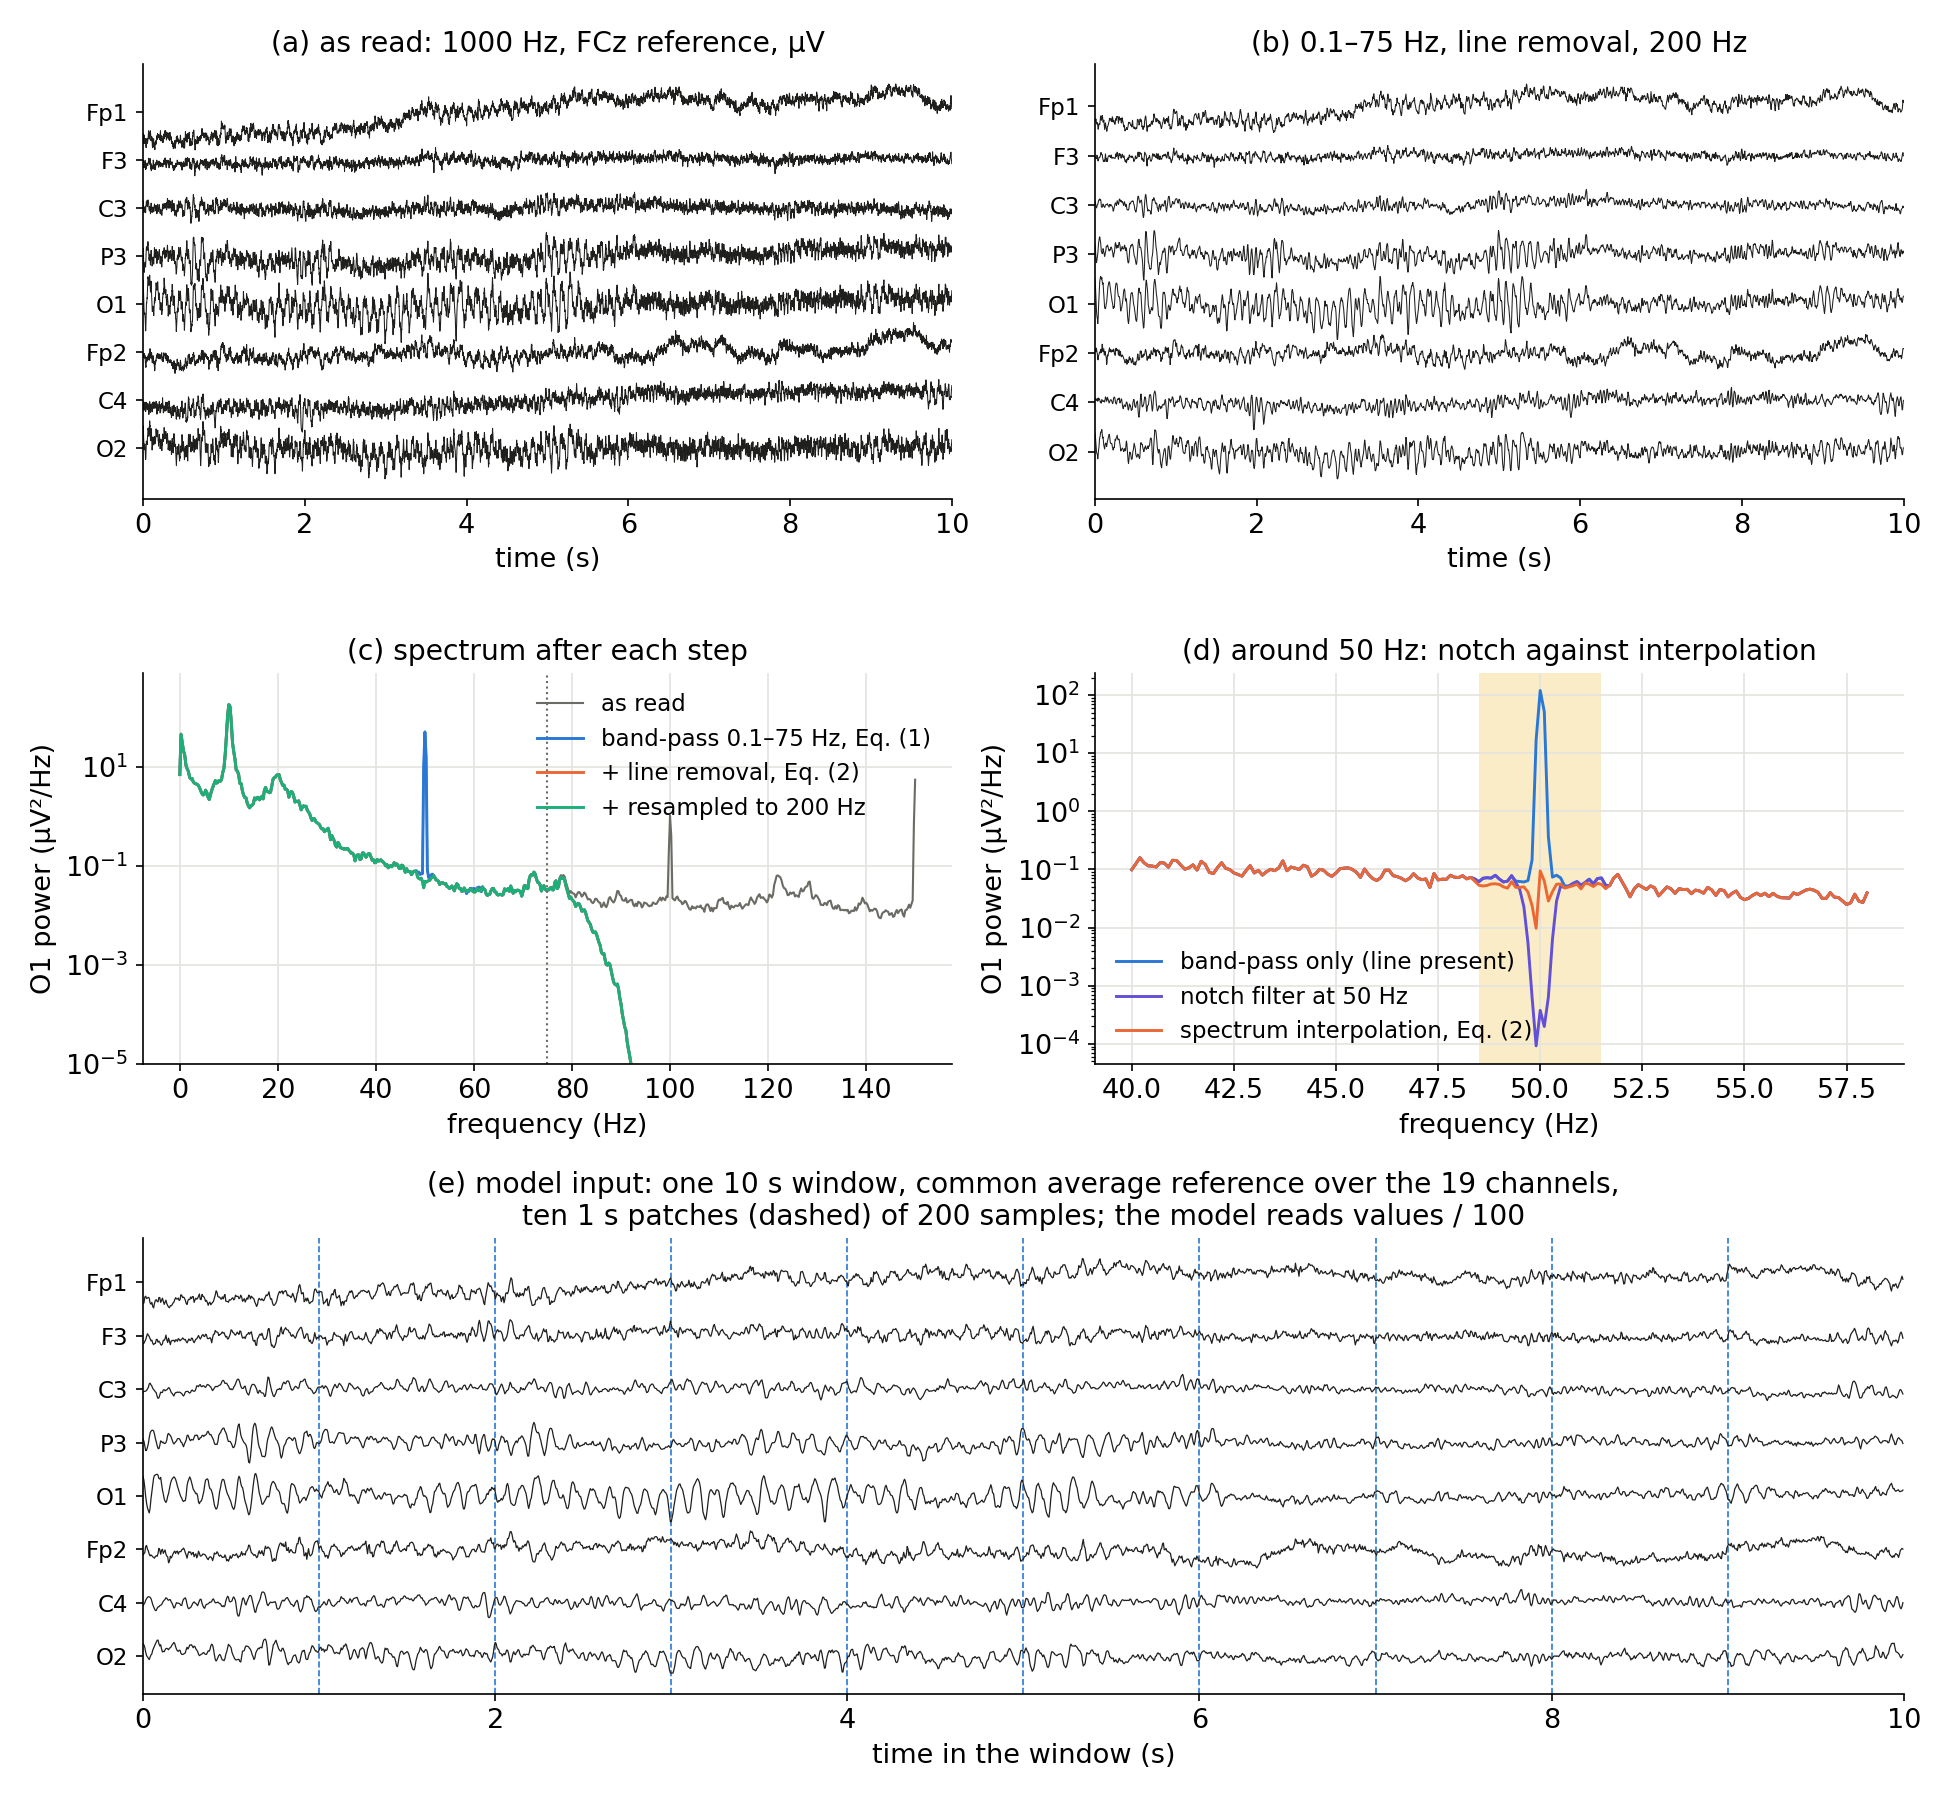
\includegraphics[width=\textwidth,height=0.62\textheight,keepaspectratio]{fig_preprocessing.png}
\caption{The preprocessing on one recording, the same 10 s of a Dortmund participant (eyes closed, 19 channels, recorded at 1,000 Hz against FCz; open data, CC0). (a) As read (DC offset removed by the reader). (b) After the band-pass, Eq. (1), line removal at 50 and 60 Hz, Eq. (2), and resampling to 200 Hz, Eq. (3). (c) Welch power spectrum of O1 (4 s segments, the whole recording) after each step: the band-pass removes the power above 75 Hz and the 100 Hz harmonic, line removal the 50 Hz line, and resampling leaves 0--100 Hz. (d) The same around 50 Hz (10 s segments): a notch filter (MNE \texttt{notch\_filter}, the published TUAB recipe) cuts a hole of three orders of magnitude into the spectrum, spectrum interpolation brings the line down to the level of its neighbours; shaded: the $\pm$1.5 Hz band of Eq. (2). (e) The model input of Eq. (5): the window after the common average reference, with the ten 1 s patches that become the encoder's tokens. 8 of 19 channels; traces 75 $\mu$V apart and clipped at $\pm$71 $\mu$V for display (the stored signal is not clipped). \texttt{scripts/tech\_report\_figures.py}.}
\end{figure}


\subsection{Data splits and cross-validation}

\textbf{One patient split.} Each corpus is split by patient, never by recording (Table 5). Temple keeps the official TUAB evaluation split as its test set (274 recordings), and every other recording of those patients is removed from training. The remaining Temple patients are split into training and a seeded validation share; the patient split is shared by every Temple cohort of this project, so a model can be scored on another cohort's validation set without leakage (\texttt{dataset\_maker/tueg\_patient\_split.py}). Harvard draws 10 \% test and 10 \% validation patients by a hash of the BDSP patient identifier, which is the same for a patient seen at several sites. No patient is in two splits of either corpus, and no patient identifier is shared between the corpora (\texttt{dataset\_maker/make\_joint\_cohort.py} checks both).

\begin{table}[t]
\centering
\small
\caption{Splits of the training cohort \texttt{tuh\_heedb\_v1}. Recordings, patients, 10 s windows (millions) and mean age in years; report verdict as a percentage of the recordings.}
\resizebox{\textwidth}{!}{%
\begin{tabular}{lllllll}
\toprule
\textbf{corpus} & \textbf{split} & \textbf{recordings} & \textbf{patients} & \textbf{windows} & \textbf{age, mean} & \textbf{normal / abnormal report} \\
\midrule
Temple & train & 27,616 & 12,194 & 5.33 M & 52.4 & 38.8 / 53.6 \% \\
Temple & validation & 3,422 & 1,533 & 0.71 M & 52.1 & 40.6 / 49.0 \% \\
Temple & test (TUAB evaluation) & 274 & 251 & 0.04 M & 50.4 & 54.4 / 45.6 \% \\
Harvard & train & 57,275 & 46,010 & 12.95 M & 53.9 & 20.0 / 30.6 \% \\
Harvard & validation & 7,192 & 5,841 & 1.64 M & 54.1 & 20.8 / 30.3 \% \\
Harvard & test & 7,338 & 5,827 & 1.66 M & 54.1 & 20.7 / 30.7 \% \\
both & train / validation / test & 84,891 / 10,614 / 7,612 & 58,204 / 7,374 / 6,078 & 18.29 / 2.35 / 1.69 M &  &  \\
\bottomrule
\end{tabular}
}
\end{table}


\textbf{Cross-validation.} The ensembles of Section 4.4 pool the training and validation patients of both corpora (95,505 recordings) and divide them into five folds by patient, seeded, about 13,200 patient groups and 1.9 M windows per fold; Temple and Harvard patients are mixed in every fold. Fold model $k$ trains on the four other folds and selects its epoch on fold $k$. The test split of Table 5 is the same for every fold model and is never seen in training or selection. The folds group Harvard recordings by the site-specific subject identifier, not the cross-site patient identifier: 326 of the 51,851 Harvard training and validation patients (0.6 \%, 880 recordings) were seen at two sites and fall into two folds. They can therefore be in a fold model's training and validation data at once. This touches the selection of the epoch and the out-of-fold numbers of Table 15 slightly, not the test results; later runs should group by the patient identifier.

\subsection{Test cohorts}

Table 6 lists the seven cohorts and Table 7 where each comes from, who was recorded and which recordings this report scores. The five external cohorts are converted with the same pipeline and are never used for training, model selection or calibration, and none of them is in the pre-training data of the LaBraM encoder (Section 10.4). Results are for adults (18 years or older): the training data has almost no younger patients. Test sets that are too small for a stable estimate are left out of this report: the adults of the developmental cohort MIPDB~\citep{langer2017mipdb} were scored as well, but with 31 recordings the 95 \% interval of the MAE is more than 4 years wide. Four further cohorts were scored and rejected as age benchmarks: NMT~\citep{khan2022nmt}, released band-limited, and three clinic cohorts of dementia and Parkinson's disease~\citep{miltiadous2023ahepa,singh2023iowapd,katzir2026telavivpd} whose healthy controls are predicted 7 to 11 years too young; the clinic cohorts serve only for comparisons of patients and controls inside a cohort (Section 6.6). Section 10.2 lists every cohort that was scored, with the rejected ones and the reason, and Section 10.3 gives the full table of each cohort.

\begin{table}[t]
\centering
\small
\caption{Test cohorts (adults). Temple and Harvard are the held-out test split of the training cohort; the others are external.}
\resizebox{\textwidth}{!}{%
\begin{tabular}{llllll}
\toprule
\textbf{cohort} & \textbf{role} & \textbf{n (subjects)} & \textbf{age, mean} & \textbf{population} & \textbf{recording} \\
\midrule
Temple (TUH)~\citep{obeid2016tuh} & in-domain test & 272 recordings (249) & 50.7 & hospital, routine EEG; 149 normal and 123 abnormal reports & about 20 min \\
Harvard (HEEDB)~\citep{heedb} & in-domain test & 7,338 recordings (5,884) & 54.1 & hospital, routine EEG; 1,518 normal, 2,253 abnormal, 3,567 without verdict & about 30 min \\
TDBRAIN~\citep{vandijk2022tdbrain} & zero-shot & 1,113 sessions (1,062) & 45.2 & psychiatric outpatients (MDD, ADHD, OCD, memory complaints) and 179 healthy controls & 2 min eyes closed + 2 min eyes open \\
LEMON~\citep{babayan2019lemon} & zero-shot & 214 recordings (214) & 39.2 & healthy volunteers, 20--80 years, ages in 5-year bins & 16 min, eyes closed / open \\
Dortmund Vital Study~\citep{wascher2025dortmund,gajewski2022dortmund} & zero-shot & 816 sessions (608) & 46.1 & healthy volunteers, 20--70 years, exact ages; 208 recorded again after about 5 years & four 3-min runs per session: eyes closed and open, before and after a 2-hour block of cognitive tasks \\
SRM~\citep{hatlestadhall2021srm} & zero-shot & 152 recordings (110) & 38.8 & healthy volunteers, adults to 71 years; 42 with a second session & 4 min eyes closed \\
CHBP~\citep{valdessosa2021chbp} & zero-shot & 250 recordings (250) & 31.7 & healthy volunteers, 18--68 years & about 19 min resting, recorded 0.5--50 Hz \\
\bottomrule
\end{tabular}
}
\end{table}


\begin{table}[t]
\centering
\small
\caption{Source, recruitment and selection of the test cohorts. Criteria as published by each data release or study protocol; \texttt{selection}: what this report scores (adults, 18 years or older, in every cohort).}
\resizebox{\textwidth}{!}{%
\begin{tabular}{lllll}
\toprule
\textbf{cohort} & \textbf{source} & \textbf{who was recorded: recruitment and criteria} & \textbf{recording system} & \textbf{selection in this report} \\
\midrule
Temple & Temple University Hospital, Philadelphia, USA; TUH EEG Corpus, TUAB v3.0.1 release~\citep{obeid2016tuh} & patients referred for a routine clinical EEG (in- and outpatients, any indication); every session of the TUAB evaluation set is labelled normal or abnormal from the neurologist's report & clinical EEG systems, 250--1,000 Hz, average or linked-ears montage (Table 2) & the official TUAB evaluation split, a patient-disjoint test set: 272 of its 274 recordings \\
Harvard & four hospital sites of the Brain Data Science Platform (BDSP), USA; HEEDB v4.1~\citep{heedb}; institutions are not named per site (Table 3) & patients referred for a routine clinical EEG, adults 18--89; continuous, intensive-care, epilepsy-monitoring and operating-room recordings excluded; report verdict from the BDSP report findings where the site provides one & clinical EEG systems, 200--512 Hz, as exported by each site (Table 2) & 10 \% of the patients, drawn by a hash of the cross-site patient identifier: 7,338 recordings \\
TDBRAIN & Brainclinics, Nijmegen, the Netherlands; one site, recorded 2001--2021; release 3.1~\citep{vandijk2022tdbrain} & psychiatric outpatients referred to the clinic for assessment or treatment, with a DSM-5 diagnosis or a referral indication (major depression, ADHD, OCD, subjective memory complaints and smaller groups), and healthy controls & 26 channels (Compumedics Quik-Cap or ANT Waveguard), 500 Hz, DC to 100 Hz, averaged-mastoid reference & the 2-min eyes-closed and eyes-open rest files of every adult session (4 sessions have the eyes-closed file only): 1,113 sessions of 1,062 people; a session's prediction is the mean of its files \\
LEMON & Max Planck Institute for Human Cognitive and Brain Sciences, Leipzig, Germany~\citep{babayan2019lemon} & volunteers from the Leipzig area in a young (20--40) and an old (55--80) group, screened healthy: no neurological, psychiatric or cardiovascular disease, cancer or drug use (the same people have MRI); public ages in 5-year bins & BrainAmp (Brain Products), 61 channels, 2,500 Hz, FCz reference & 214 of 215 recordings (one is 80 s long) \\
Dortmund & Leibniz Research Centre for Working Environment and Human Factors (IfADo), Dortmund, Germany; Dortmund Vital Study, NCT05155397~\citep{wascher2025dortmund,gajewski2022dortmund} & working-age adults 20--70, recruited from local companies, public institutions and advertisements in newspapers and other media; excluded: neurological disease (dementia, Parkinson's, stroke), cardiovascular, oncological, eye, psychiatric and affective disease, head injury, surgery or implants, psychotropic drugs and neuroleptics, limited mobility & BrainAmp DC, actiCAP 64 channels, 1,000 Hz, FCz reference & every session: 816 sessions of 608 people, 208 of them recorded again after about 5 years; a session's prediction is the mean of its four runs \\
SRM & Department of Psychology, University of Oslo, Norway; healthy control group of the Stimulus-Selective Response Modulation project~\citep{hatlestadhall2021srm} & healthy adults 17--71 with cognitive testing at the first session; 42 recorded again 2--13 months later & BioSemi ActiveTwo, 64 channels, 1,024 Hz, unfiltered, released average-referenced & 152 of 153 recordings (one participant is 17) \\
CHBP & Cuban Neuroscience Center, Havana, Cuba; Cuban Human Brain Mapping Project~\citep{valdessosa2021chbp} & a population-based sample of healthy adults aged 18--68 & MEDICID-5, 120 channels, 200 Hz, recorded 0.5--50 Hz with a 60 Hz notch & the 250 people with an EEG in release 1.0 (of 282; the others have MRI only); the resting part before hyperventilation \\
\bottomrule
\end{tabular}
}
\end{table}


The two hospital cohorts record patients as they come to the clinic, with their medication, drowsiness and artifacts, and TDBRAIN psychiatric outpatients under a fixed research protocol; LEMON, Dortmund, SRM and CHBP screen out disease and record alert, seated volunteers in a laboratory. Table 8 and Figure 2 show how this difference appears in the signal, and Section 6.5 how a recording system alone can shift the predictions (CHBP).

\subsection{Dataset analytics}

Table 8 and Figure 2 compare the seven cohorts on who was recorded and on what the models see. The signal features are computed per recording on the model input (19 channels, common average reference, $\mu$V at 200 Hz; first 5 minutes after the cohort's trims), per 10 s window and then as the median over windows (\texttt{scripts/domain\_shift\_analysis.py}, \texttt{scripts/dataset\_analytics.py}). For Temple and Harvard they come from validation recordings with a normal report aged 18 to 68 (1,198 and 1,233 recordings), the label-free reference of Section 6.5; for Dortmund they are per run. Signal features are medians over recordings.

\begin{table}[t]
\centering
\small
\caption{Demographics and signal features of the report cohorts; units as in Table 6. Age in years, mean $\pm$ standard deviation; \texttt{men} and \texttt{healthy} in \% (healthy: normal EEG report for Temple and Harvard, healthy volunteer or control otherwise). Signal features are medians over recordings (Figure 2 shows their spread): \texttt{SD}, the median channel standard deviation in $\mu$V; \texttt{artifact}, the share of windows with a channel standard deviation above 100 $\mu$V, \%; \texttt{delta} and \texttt{alpha}, relative power of 1--4 and 8--13 Hz in the 1--45 Hz band, \%; \texttt{45--70}, absolute power at 45--70 Hz in $\mu$V$^2$/Hz; \texttt{exp.}, the slope of the aperiodic 1/f fit over 2--40 Hz. Per-cohort interquartile ranges: \texttt{docs/data/external\_eval/tech\_report/dataset\_analytics.csv}.}
\resizebox{\textwidth}{!}{%
\begin{tabular}{llllllllll}
\toprule
\textbf{cohort} & \textbf{age} & \textbf{men} & \textbf{healthy} & \textbf{SD} & \textbf{artifact} & \textbf{delta} & \textbf{alpha} & \textbf{45--70} & \textbf{exp.} \\
\midrule
Temple & 50.7 $\pm$ 17.9 & 46 & 55 & 9.7 & 3 & 40 & 17 & 0.033 & 1.29 \\
Harvard & 54.1 $\pm$ 19.8 & 49 & 21 & 12.3 & 17 & 46 & 16 & 0.029 & 1.36 \\
TDBRAIN & 45.2 $\pm$ 15.9 & 49 & 16 & 9.0 & 0 & 32 & 23 & 0.039 & 1.24 \\
LEMON & 39.2 $\pm$ 20.3 & 63 & 100 & 8.8 & 0 & 41 & 19 & 0.033 & 1.32 \\
Dortmund & 46.1 $\pm$ 14.7 & 38 & 100 & 10.2 & 0 & 38 & 18 & 0.050 & 1.20 \\
SRM & 38.8 $\pm$ 13.5 & 38 & 100 & 13.1 & 0 & 33 & 32 & 0.040 & 1.28 \\
CHBP & 31.7 $\pm$ 9.3 & 71 & 100 & 5.8 & 0 & 25 & 44 & 0.001 & 1.70 \\
\bottomrule
\end{tabular}
}
\end{table}


\begin{figure}[t]
\centering
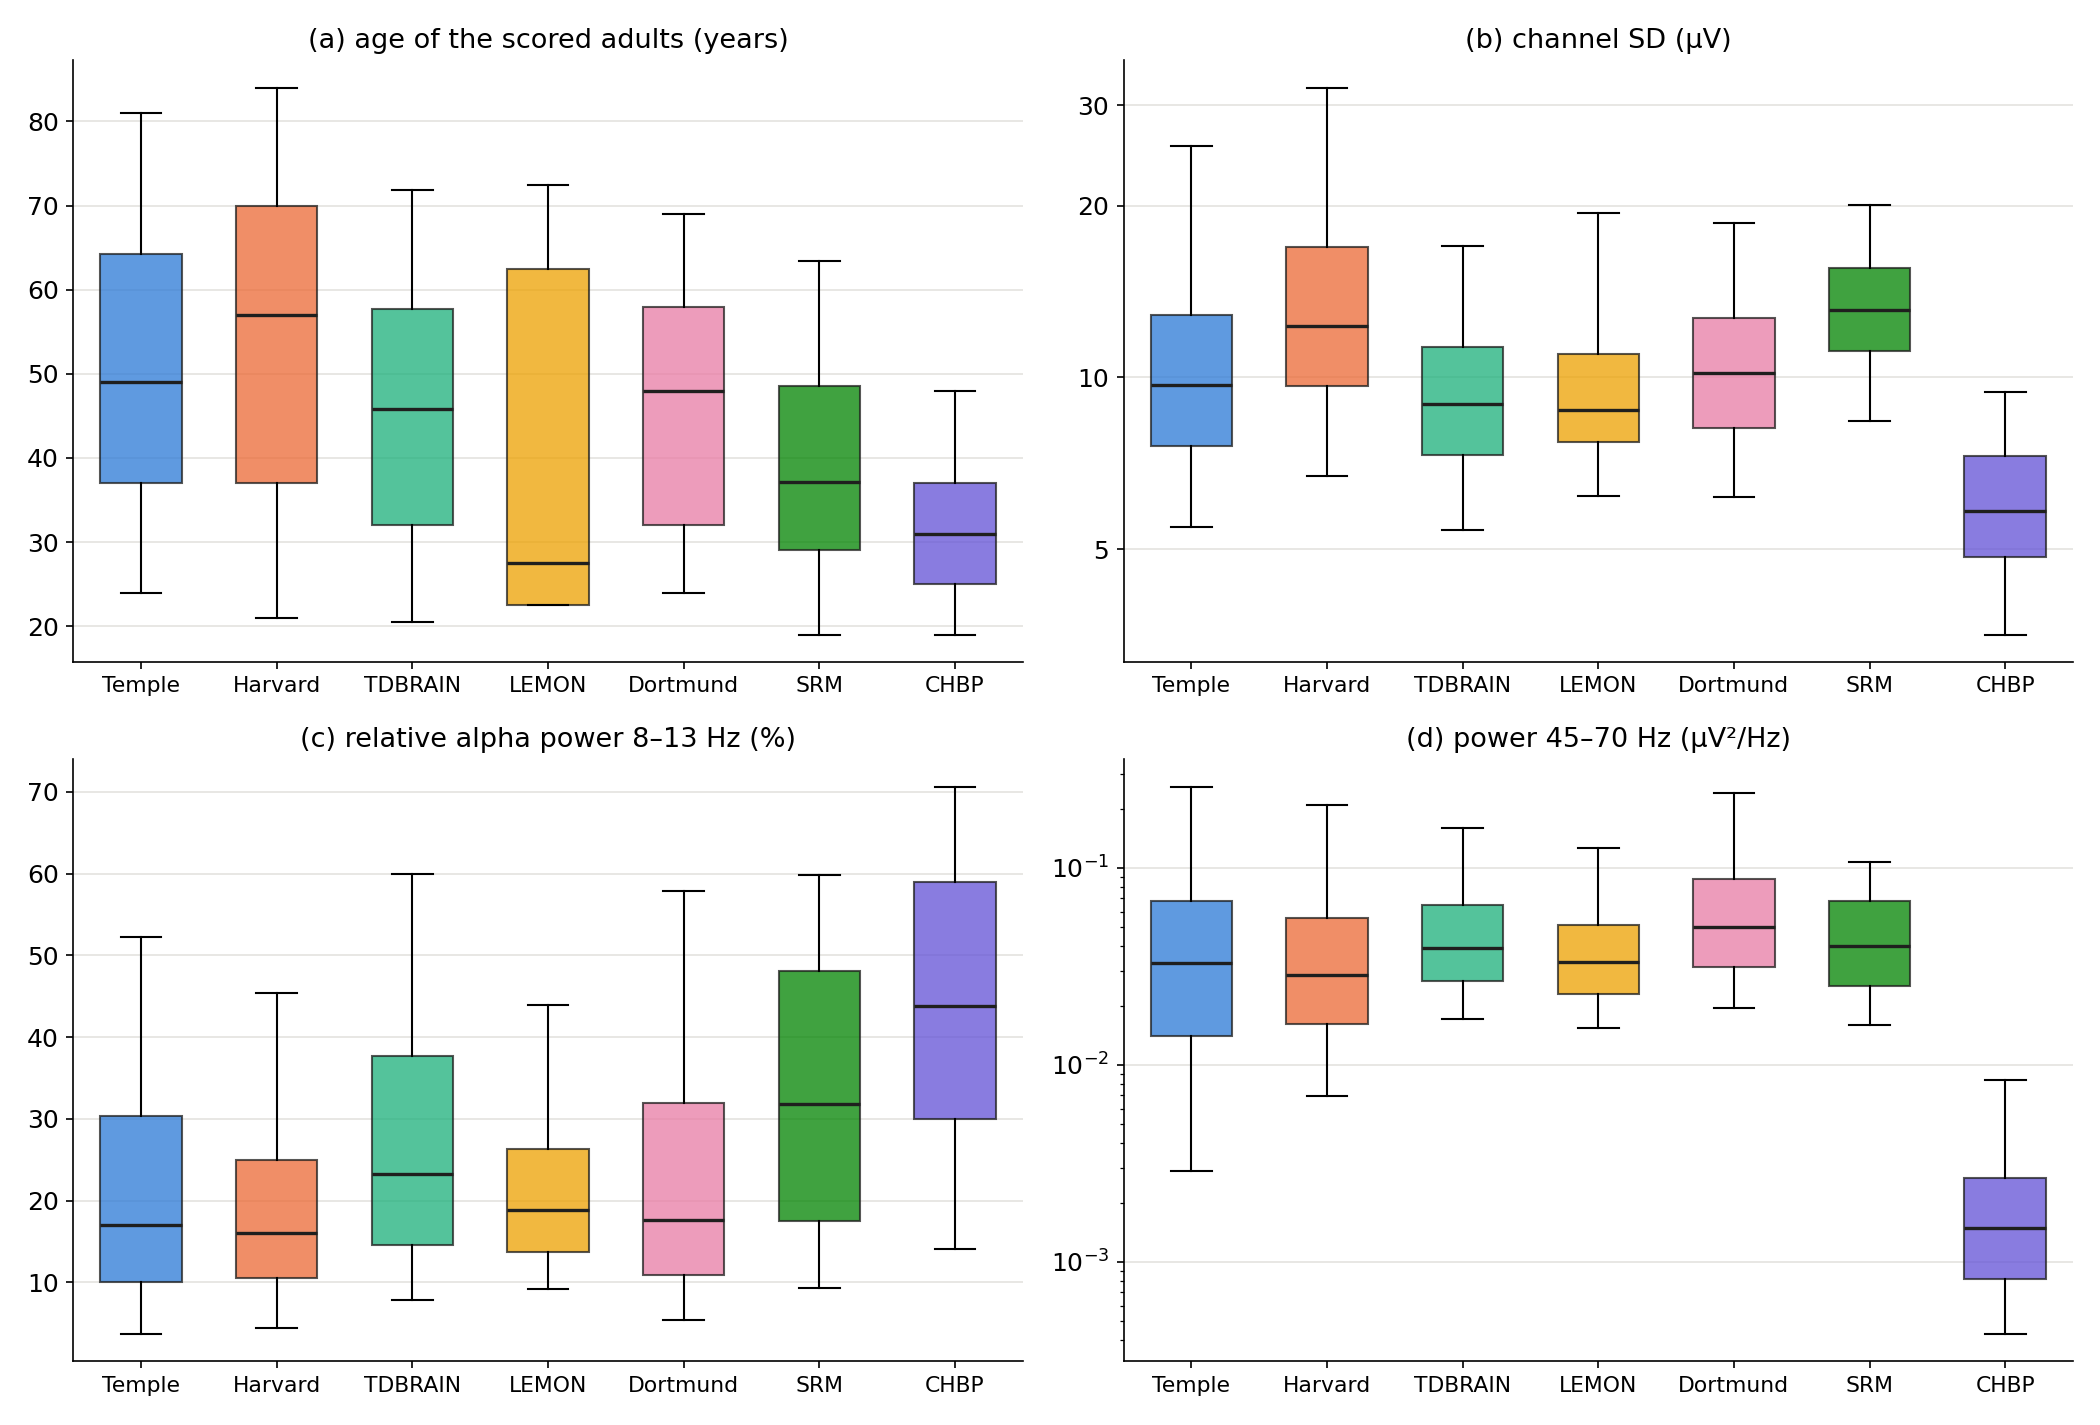
\includegraphics[width=\textwidth,height=0.62\textheight,keepaspectratio]{fig_dataset_analytics.png}
\caption{Dataset analytics of the report cohorts: (a) age of the scored adults, (b) median channel standard deviation, (c) relative alpha power, (d) absolute power at 45--70 Hz (log scales in (b) and (d)). Boxes: interquartile range and median; whiskers: 5th and 95th percentiles; no single recordings are drawn. Signal features as in Table 8.}
\end{figure}


What Table 8 and Figure 2 show:

\begin{itemize}
\item \textbf{Ages differ by design.} The hospital cohorts are the oldest (median about 50 to 57 years) and widest; CHBP is young and narrow (31.7 $\pm$ 9.3 years), which by itself caps its $R^2$. LEMON is two groups, 20--35 and 55--77 years (Figure 2(a)).
\item \textbf{Hospital and research recordings differ in artifacts and amplitude.} A median 17 \% of a Harvard recording's windows hold a channel above 100 $\mu$V (Temple 3 \%), against almost none in the research cohorts. Harvard also has the largest amplitude (12.3 $\mu$V) and the most slow-wave power (relative delta 46 \%), as expected for clinical EEG with drowsiness.
\item \textbf{The research cohorts are alert and alpha-rich.} Relative alpha is 18 to 32 \% in TDBRAIN, LEMON, Dortmund and SRM against 16 to 17 \% in the hospital references. The models still score these cohorts at or below their in-domain error (Table 13), so an alert state alone does not shift the predicted age much.
\item \textbf{CHBP is outside the training range on two axes at once:} the lowest amplitude (5.8 $\mu$V, half of Temple's) and almost no power above 45 Hz (0.001 against 0.03 $\mu$V$^2$/Hz), from its 50 Hz recording low-pass, with the steepest aperiodic slope. These are the two causes that Section 6.5 tests and corrects. No other cohort is outside the training range on amplitude or band.
\end{itemize}

\subsection{Patients with more than one recording}

A patient can contribute several recordings: Temple keeps up to 10 per patient in training, Harvard has repeat visits (Table 9). Two questions follow. How far apart in age are a patient's recordings, which matters because all recordings of a patient share one split and one cross-validation fold (Section 3.3)? And does the predicted age move with the age difference between them, a within-person check of what the cross-sectional evaluation measures across people (Table 10, Figure 3)? \texttt{scripts/repeat\_recordings\_analysis.py}; aggregates only.

\begin{table}[t]
\centering
\small
\caption{Patients with more than one recording in the training cohort \texttt{tuh\_heedb\_v1} (all splits). Age span: the age at a patient's last recording minus the age at the first, in whole years.}
\begin{tabular}{lll}
\toprule
\textbf{} & \textbf{Temple} & \textbf{Harvard} \\
\midrule
patients with $\ge$ 2 recordings & 5,225 of 13,978 (37 \%) & 9,780 of 57,678 (17 \%) \\
their recordings & 22,559 (72 \% of all) & 23,907 (33 \% of all) \\
recordings per such patient, median (90th percentile; maximum) & 3 (10; 10, the cap of the cohort) & 2 (3; 12) \\
all recordings of one visit & 18 \% & 2 \% \\
age span, mean / median / 90th percentile (years) & 2.2 / 0 / 8 & 2.4 / 1 / 7 \\
age span 0 / $\le$ 1 / $\ge$ 5 / $\ge$ 10 years & 55 \% / 67 \% / 18 \% / 7 \% & 38 \% / 58 \% / 19 \% / 5 \% \\
share of patients with $\ge$ 2 recordings: train / validation / test & 38 \% / 39 \% / 7 \% & 17 \% / 16 \% / 17 \% \\
age span inconsistent with the recording years (> 2 years off) / two sexes & 144 / 19 patients & not checkable (no recording year) \\
\bottomrule
\end{tabular}
\end{table}


\begin{table}[t]
\centering
\small
\caption{Patients recorded at different ages in a scored set: the change of the predicted age between the youngest and the oldest recording, $\Delta\hat y$, against the age difference $\Delta y$. \texttt{slope}: least-squares slope of $\Delta\hat y$ on $\Delta y$ through the origin (1 = the model follows ageing fully; the cross-sectional slopes of the P4 ensemble in Table 19 are 0.79 to 0.89 on the cohorts that resemble the training data); \texttt{older}: share of patients predicted older at the later recording (P4 ensemble). In-domain sets: first 5 minutes; external: every window.}
\resizebox{\textwidth}{!}{%
\begin{tabular}{llllll}
\toprule
\textbf{set} & \textbf{patients} & \textbf{mean $\Delta y$} & \textbf{E2L: mean $\Delta\hat y$ / slope} & \textbf{P4 ensemble: mean $\Delta\hat y$ / slope} & \textbf{older} \\
\midrule
Harvard, test patients & 615 & 3.9 & +2.4 / 0.67 & +3.0 / 0.78 & 66 \% \\
Dortmund (sessions) & 208 & 5.2 & +4.3 / 0.83 & +4.3 / 0.83 & 89 \% \\
TDBRAIN (sessions) & 40 & 1.7 & $-$0.7 / $-$0.57 & $-$0.2 / $-$0.46 & 52 \% \\
SRM & 42 & 0.7 & +0.5 / 1.12 & +1.0 / 1.58 & 55 \% \\
Temple, test patients & 14 & 2.4 & +5.2 / 0.02 & +5.7 / 0.11 & 79 \% \\
\bottomrule
\end{tabular}
}
\end{table}


\begin{figure}[t]
\centering
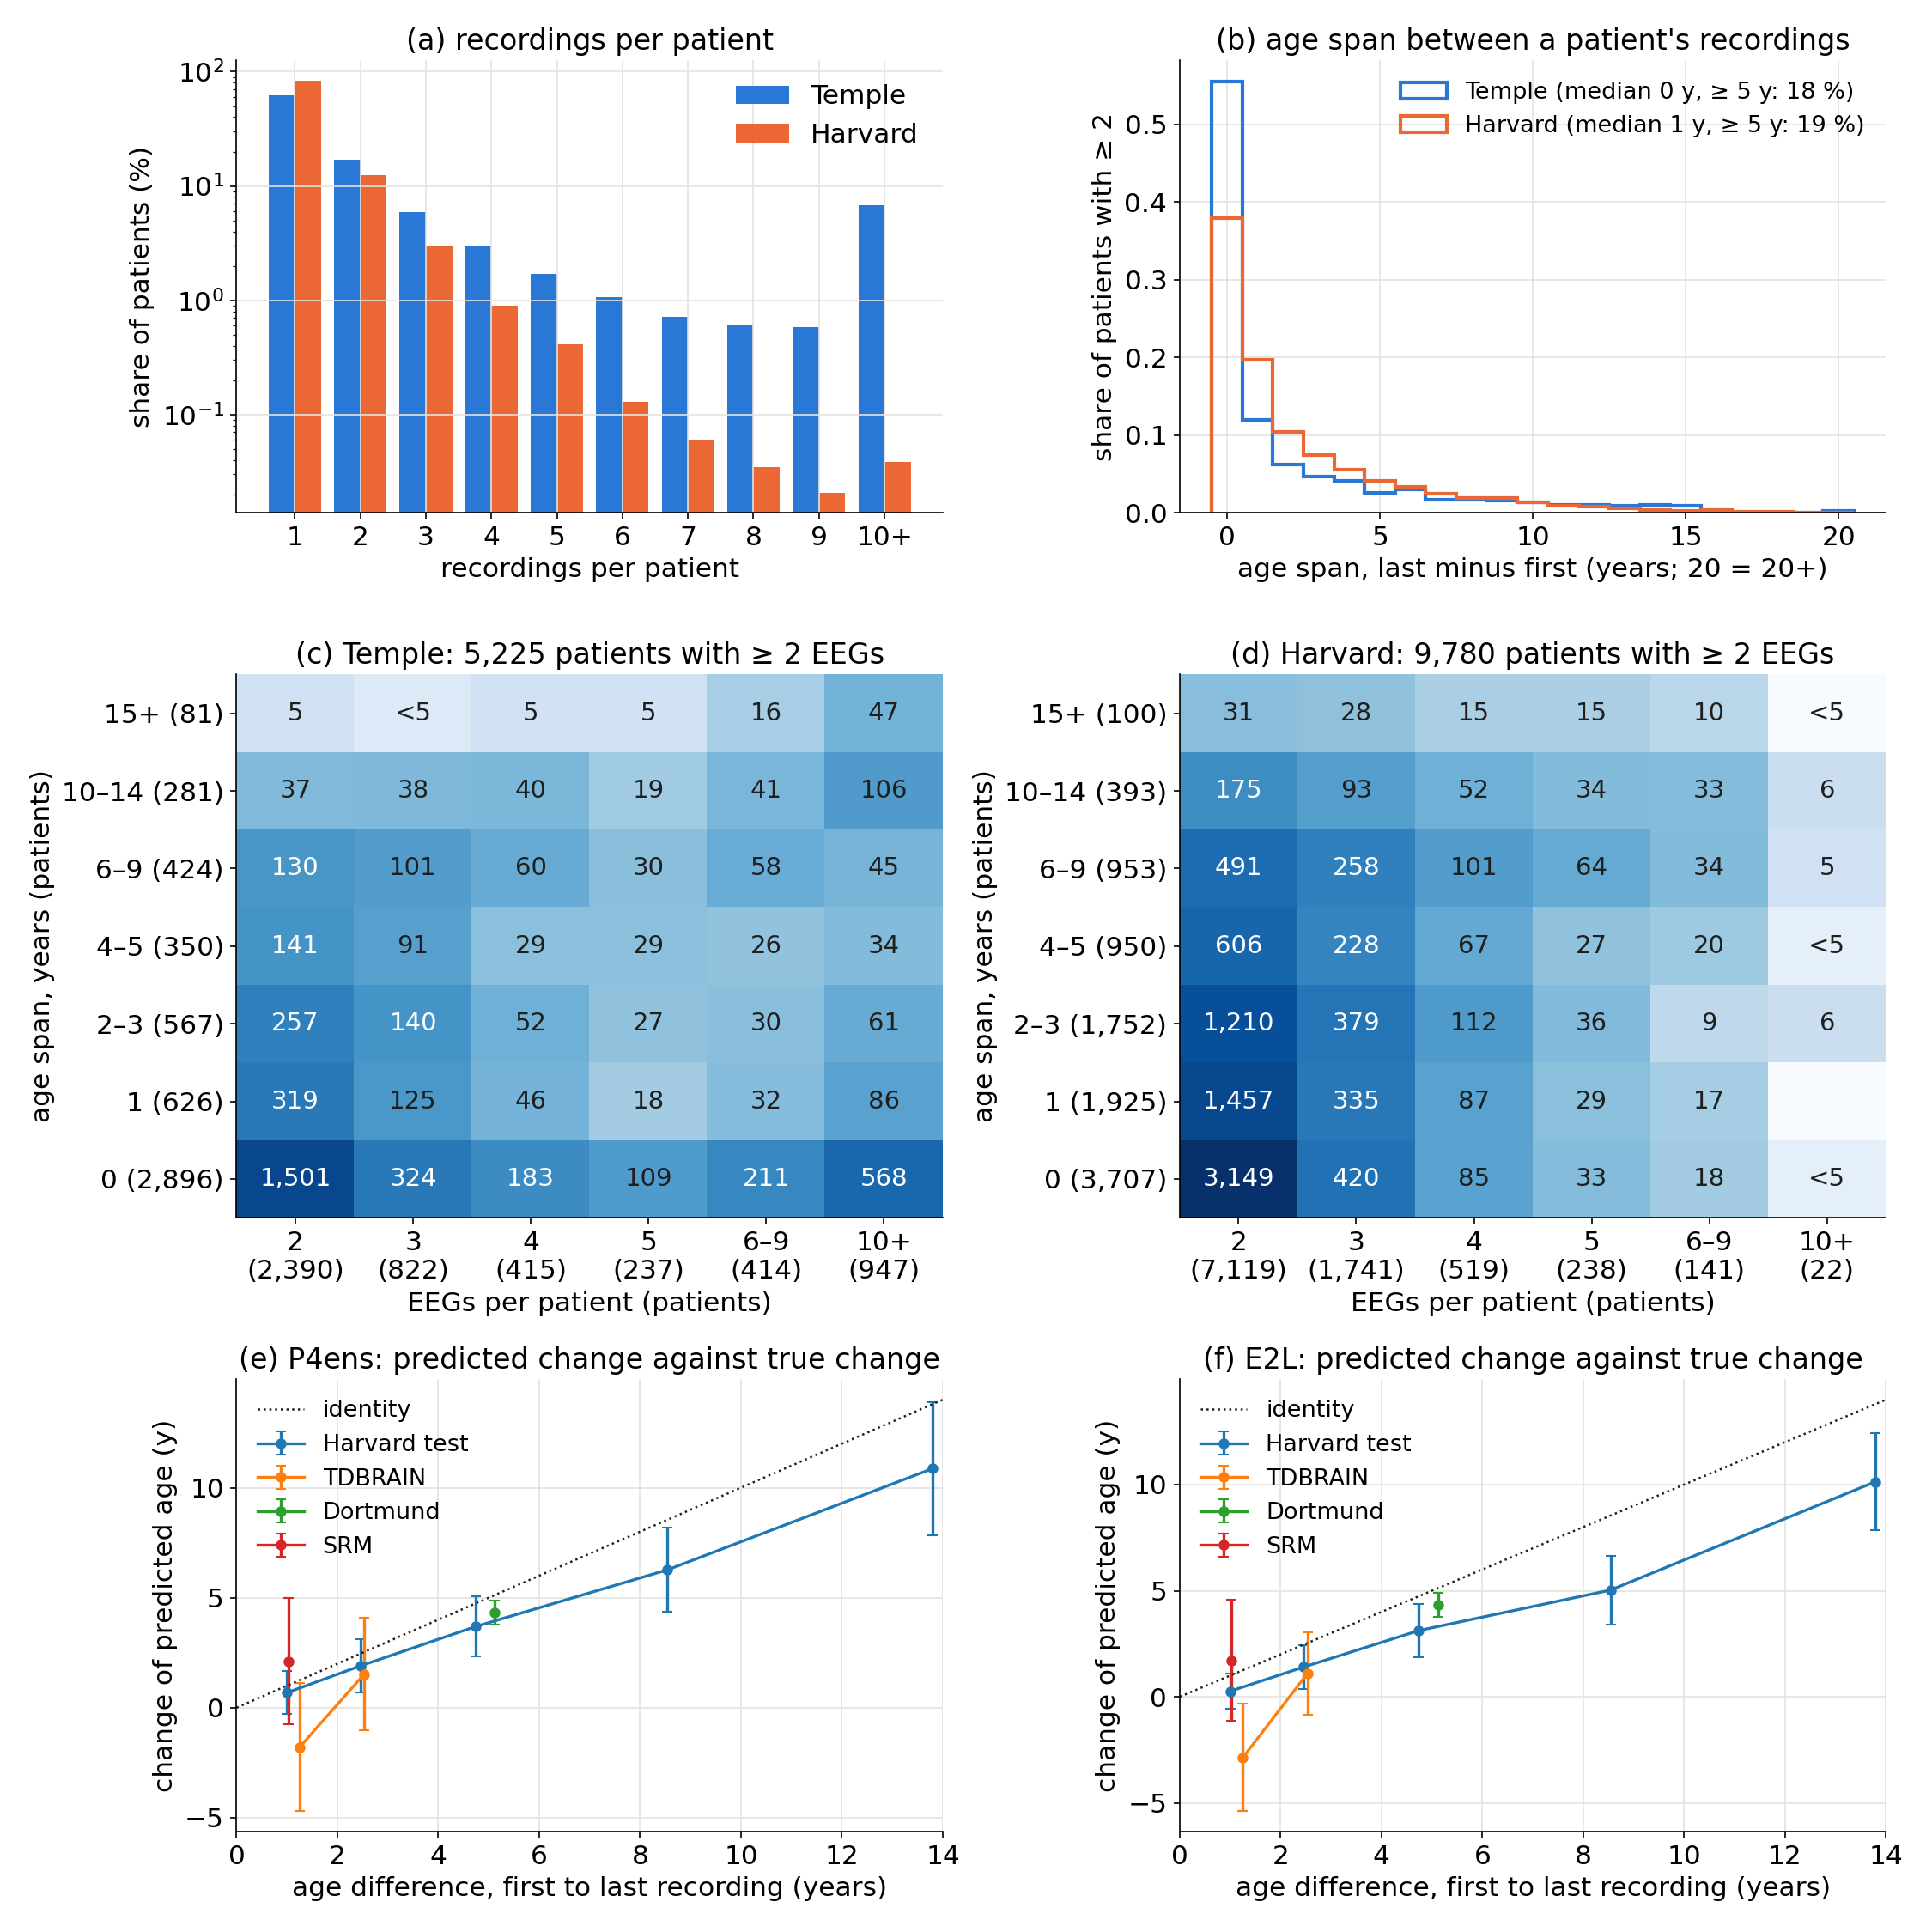
\includegraphics[width=\textwidth,height=0.62\textheight,keepaspectratio]{fig_repeat_recordings.png}
\caption{Patients with more than one recording. (a) Recordings per patient (share of patients, log scale; Temple is capped at 10 per patient). (b) Age span between a patient's first and last recording, patients with at least 2 recordings (20 = 20 or more). (c) Temple and (d) Harvard: patients with at least 2 recordings by the number of EEGs (the first and its follow-ups) and the age span they cover, all splits; in brackets the row and column totals; colour on a log scale; cells with 1 to 4 patients shown as <5 (data use agreements). Temple's cohort keeps at most 10 recordings per patient, so its 10+ column is exactly 10. (e) P4 ensemble and (f) E2L: mean change of the predicted age per band of the age difference between a patient's youngest and oldest recording (bands of 1, 2--3, 4--6, 7--10 and 11 or more years, at least 10 patients each), with 95 \% intervals; dotted: identity. Harvard: held-out test patients; TDBRAIN, Dortmund, SRM: repeat sessions.}
\end{figure}


What Tables 9 and 10 and Figure 3 show:

\begin{itemize}
\item \textbf{Repeat recordings are common, but mostly close in age.} 37 \% of Temple and 17 \% of Harvard patients have two or more recordings, holding 72 \% and 33 \% of the recordings. The median age span is 0 years in Temple, where 18 \% of such patients have all recordings in one visit, and 1 year in Harvard; 18 to 19 \% of them span 5 years or more.
\item \textbf{How many follow-up EEGs, over how many years (Figure 3(c), (d)).} Most repeat patients have one follow-up: 2,390 of 5,225 in Temple and 7,119 of 9,780 in Harvard have exactly 2 EEGs. Harvard rarely goes beyond 5 (163 patients with 6 or more), while 947 Temple patients reach the cohort's cap of 10, 568 of them within the same year of age (likely repeat sessions of one admission). Long follow-up with several EEGs is the smaller group: 823 Temple and 1,093 Harvard patients have at least 3 EEGs spanning 4 years or more, and 1,136 and 2,396 have at least 2 EEGs spanning 4 years or more. This is the material for a longitudinal model of brain-age change; the check below uses only the test patients.
\item \textbf{Temple's test split has few repeat patients} (7 \% against 38 \% in training), because it is TUAB's evaluation split; only 14 of its patients have recordings of different ages, too few for Table 10.
\item \textbf{The models follow ageing within a person.} For the 615 Harvard test patients recorded at different ages (mean 3.9 years apart) the P4 ensemble's prediction rises by 0.78 years per year, about its cross-sectional slope; E2L by 0.67. Dortmund, where 208 people were recorded about 5 years apart, gives 0.83 (Section 6.7). With intervals of 1 to 2 years (TDBRAIN, SRM) the change is within the noise of single sessions (Figure 3(e), (f)).
\item \textbf{A data-quality flag in Temple:} for 144 patients with repeat recordings the age span differs by more than 2 years from the span of their recording years, and 19 appear with two sexes, which points to header errors or reused subject codes. They are 0.5 \% of the Temple recordings and stay in the cohort.
\end{itemize}

\textbf{Repeat EEGs in the test cohorts.} Figure 4 counts the EEGs per person in the seven test cohorts as they are scored (adults; a session is the unit where a session has several files: TDBRAIN's eyes-closed and eyes-open files, Dortmund's four runs). LEMON and CHBP have one EEG per person. The two hospital test sets have repeat recordings like their training data: 18 of the 249 Temple test patients (at most 4 recordings) and 1,010 of the 5,827 Harvard test patients (708 with two, 302 with three to twelve), typically 1 year apart, in Harvard up to 7 years for 90 \% of them (Harvard patients counted by the cross-site patient identifier, which joins a patient's site-specific subject codes: 5,827 patients against the 5,884 codes of Table 6). Among the volunteer cohorts, Dortmund has the long follow-up (208 of 608 people, a second session 4 to 8 years later, median 5), SRM a short one (42 of 110, 2 to 13 months), and TDBRAIN a few repeat sessions of patients (47 of 1,062, median 1.1 years). Every unit is scored and counted on its own in the accuracy tables, and the 95 \% intervals resample people, not units, so a person's repeat EEGs do not narrow them; those recorded at different ages are the people of the within-person check in Table 10.

\begin{figure}[t]
\centering
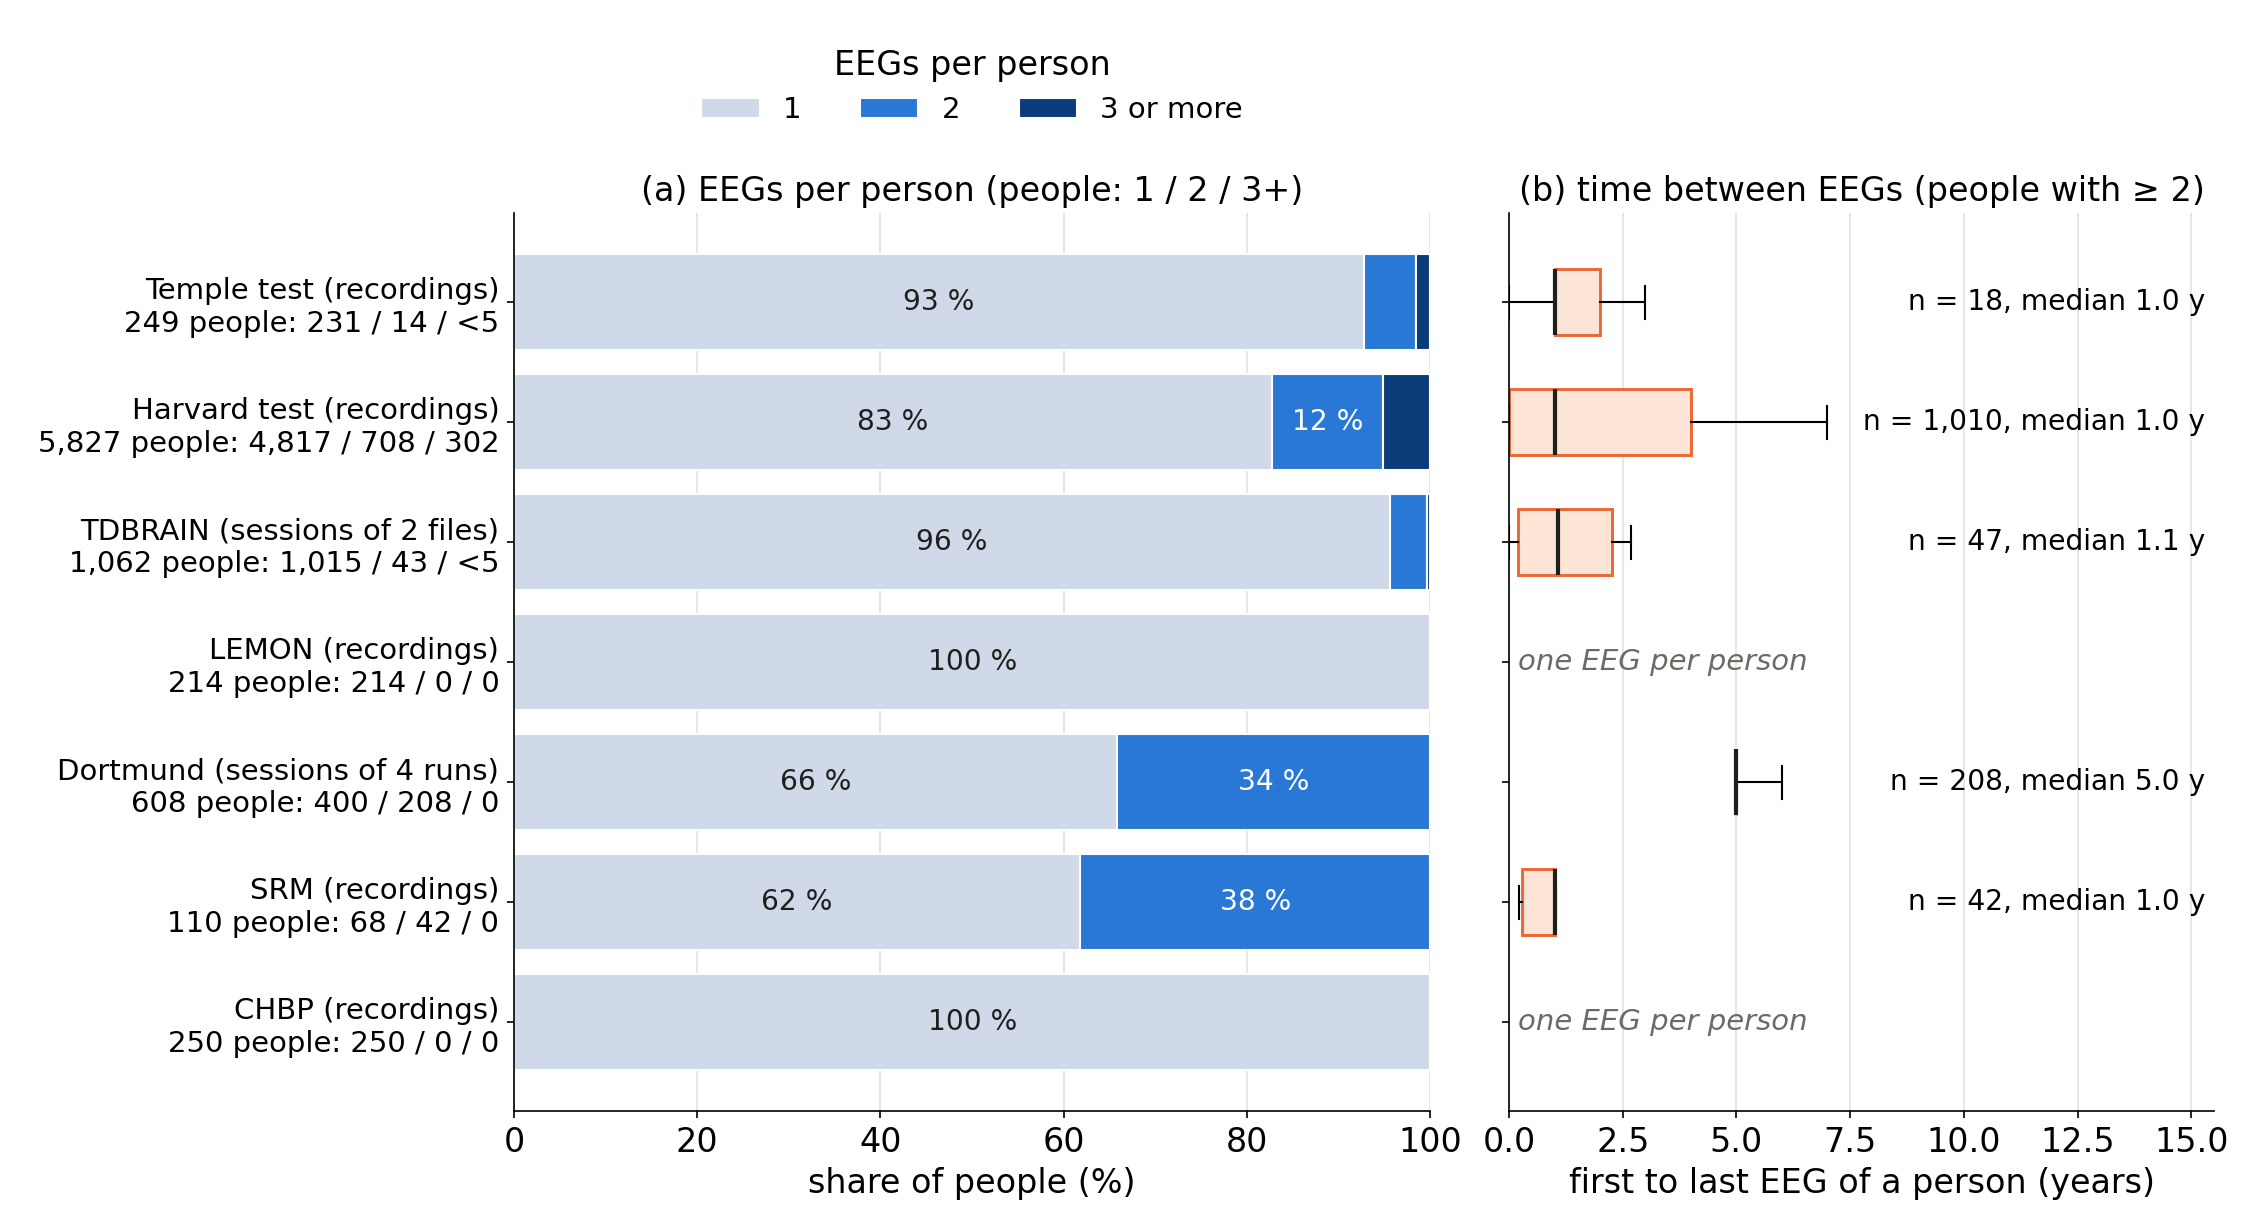
\includegraphics[width=\textwidth,height=0.62\textheight,keepaspectratio]{fig_test_repeat.png}
\caption{EEGs per person in the test cohorts, as scored (adults). (a) Share of people with 1, 2, or 3 or more EEGs; in the labels the unit and the number of people in each group (groups of 1 to 4 people shown as <5, data use agreements). (b) Time between a person's first and last EEG, people with at least 2: box = interquartile range, line = median, whiskers = 10th and 90th percentiles, from the age difference (whole years in Temple, Harvard and Dortmund; to the month or day in SRM and TDBRAIN). \texttt{scripts/repeat\_recordings\_analysis.py}; counts in \texttt{docs/data/external\_eval/tech\_report/repeat\_recordings\_test\_cohorts.csv}.}
\end{figure}


\section{Method}

Figures 5 and 6 show the whole pipeline: LaBraM's own figure of its pre-training (Figure 5) and, in the same shapes, what this work adds (Figure 6). The encoder and its pre-training are LaBraM's~\citep{jiang2024labram} and are reused unchanged. Everything after the pre-trained weights is ours (Figure 6): one preprocessing for every cohort, the common average reference, the recording-level objective with attention pooling over 10 s windows, the cross-validation ensemble and the confidence. Sections 4.1 to 4.5 define each step.

\begin{figure}[t]
\centering
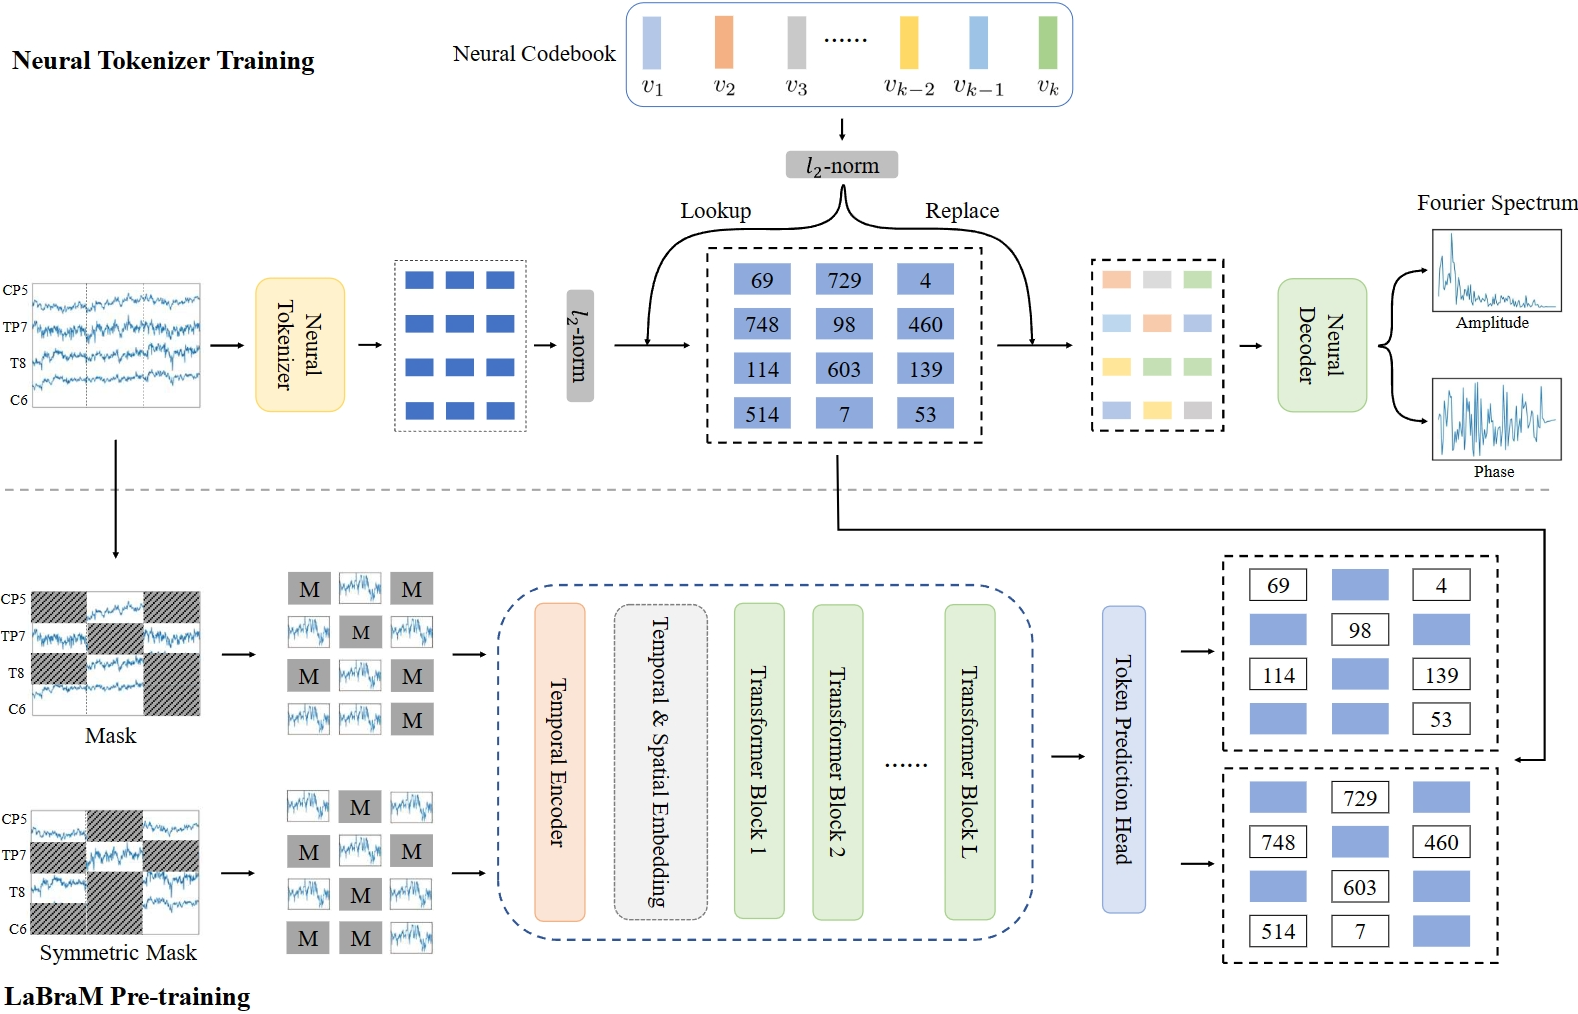
\includegraphics[width=\textwidth,height=0.62\textheight,keepaspectratio]{fig_labram_original.png}
\caption{LaBraM pre-training, the original figure of Jiang et al.~\citep{jiang2024labram} (\texttt{labram.png} of the authors' repository, MIT licence), reused as published and not retrained here. Top: the neural tokenizer learns a codebook by reconstructing the Fourier amplitude and phase of each 1 s patch. Bottom: the encoder (temporal encoder, temporal and spatial embedding, transformer blocks) learns by predicting the codes of masked patches.}
\end{figure}


\begin{figure}[t]
\centering
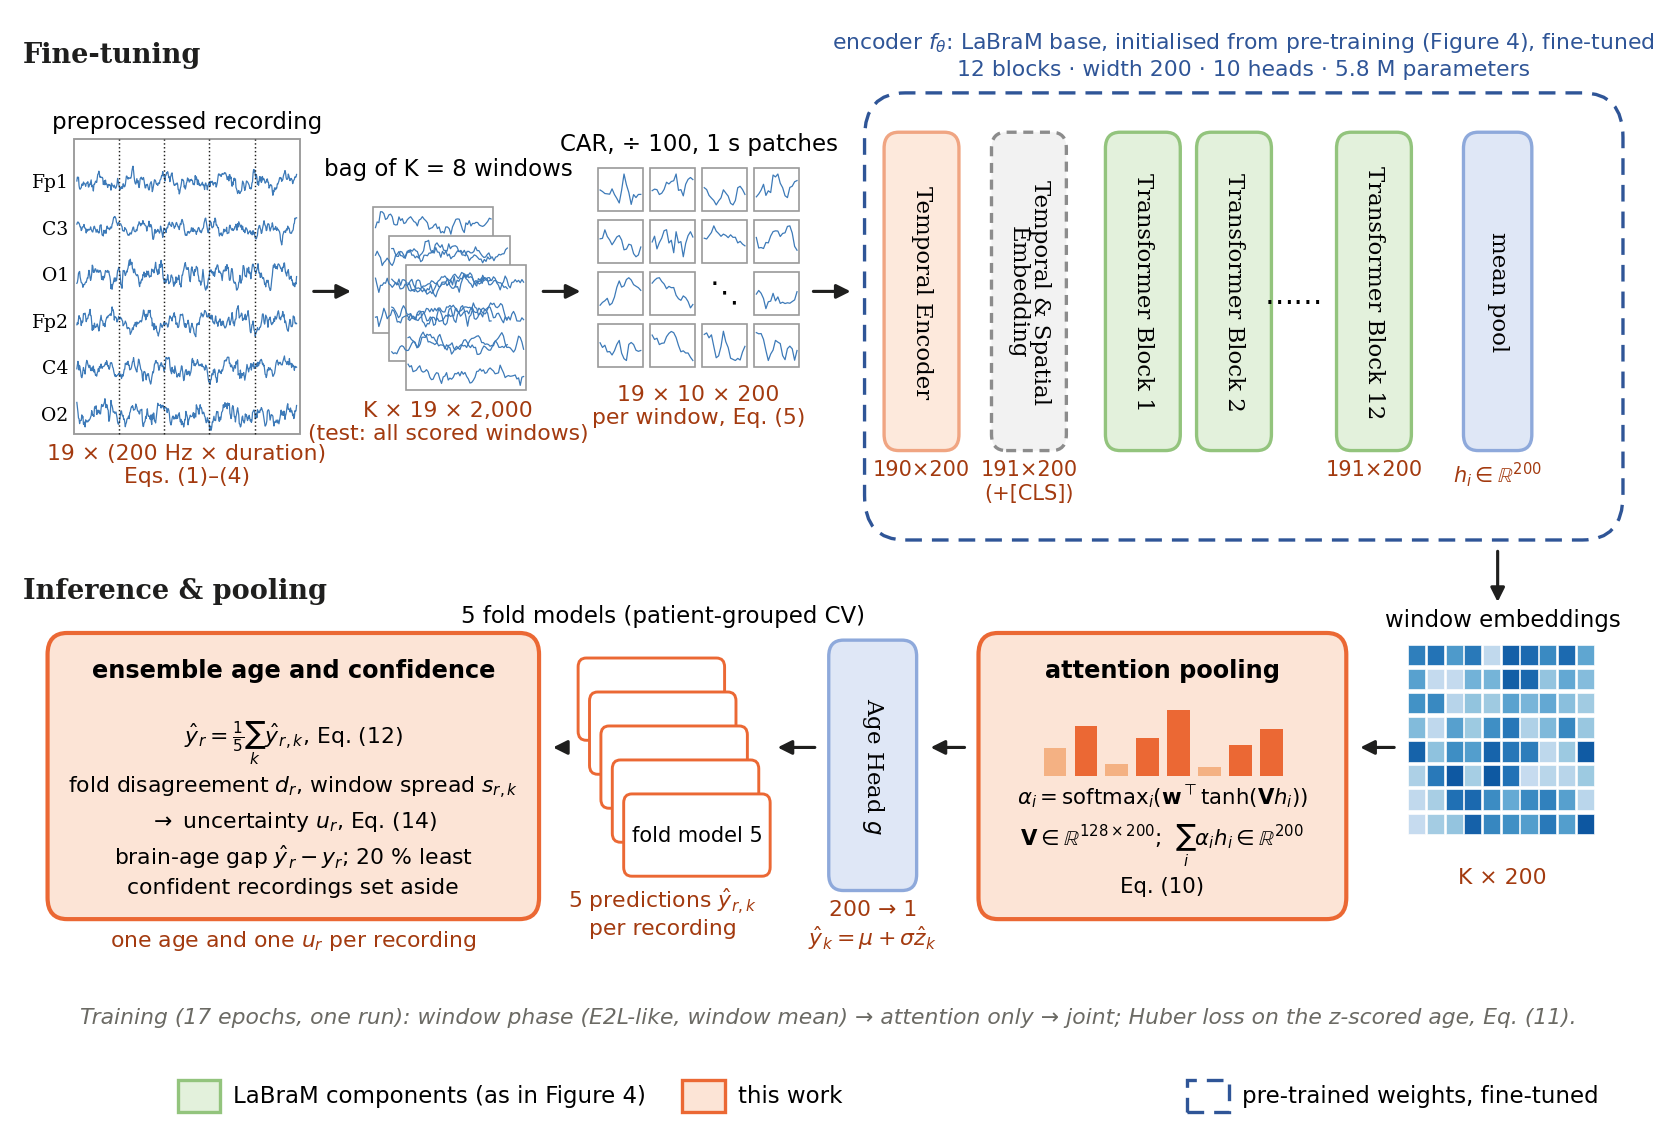
\includegraphics[width=\textwidth,height=0.62\textheight,keepaspectratio]{fig_pipeline.png}
\caption{This work, drawn in the visual language of Figure 5, with the tensor shape after each step for one recording (red). The preprocessed recording (Eqs. (1)--(4)) gives a bag of $K = 8$ random 10 s windows in training and all scored windows at test; each window is re-referenced, scaled and cut into 19 $\times$ 10 patches of 200 samples (Eq. (5)); the temporal encoder (three 1-D convolutions, kernel 15 with stride 8, then 3 and 3, 8 filters, group norm, GELU) turns every patch into a 200-d token, giving 190 tokens; a class token and the channel (spatial) and time embeddings are added; 12 transformer blocks follow, and the mean of the 190 output patch tokens is the window embedding $h_i \in \mathbb{R}^{200}$. Attention pooling (Eq. (10)) weights the $K$ embeddings, the head $g$ maps the pooled embedding to one age per recording and fold model, and the five fold models give the ensemble age (Eq. (12)) and its uncertainty (Eq. (14)). Green, grey and blue boxes: LaBraM's components with its pre-trained weights, fine-tuned; orange: this work. E2L uses the same encoder and head without the attention pooling: the mean of its window predictions, Eq. (9). \texttt{scripts/tech\_report\_figures.py}.}
\end{figure}


\subsection{Input and encoder}

A recording $r$ is a set of windows $x_{r,i} \in \mathbb{R}^{C \times T}$ with $T = 2000$ samples (10 s at 200 Hz) and the $C \le 19$ channels of the 10--20 system that the recording has. Each window is re-referenced to the common average and scaled, Eq. (5), the input variant of LaBraM++~\citep{barmpas2025labrampp} without its per-patch z-scoring. Missing channels are left out of the token sequence. The LaBraM base encoder $f_\theta$ maps a window to an embedding $h_{r,i} = f_\theta(x_{r,i}) \in \mathbb{R}^{200}$, and a linear head $g$ maps an embedding to a scalar.

\subsection{Window model (E2L)}

The target is the age $y_r$ z-scored with the training mean and standard deviation ($\mu = 53.52$, $\sigma = 19.29$ years):

\begin{equation}
z_r = \frac{y_r - \mu}{\sigma}, \qquad \hat z_{r,i} = g(h_{r,i}) \tag{6}
\end{equation}

The loss is the Huber loss~\citep{huber1964robust} with $\delta = 1$ between each window's prediction and its recording's target:

\begin{equation}
\ell_\delta(u) = \begin{cases} \frac{1}{2} u^2, & \lvert u \rvert \le \delta \\ \delta \big(\lvert u \rvert - \frac{1}{2}\delta\big), & \text{otherwise} \end{cases} \tag{7}
\end{equation}

Training uses mixup~\citep{zhang2017mixup} on inputs and targets, with one $\lambda$ per batch:

\begin{equation}
\tilde x = \lambda x_a + (1-\lambda)\,x_b, \qquad \tilde z = \lambda z_a + (1-\lambda)\,z_b, \qquad \lambda \sim \mathrm{Beta}(0.4,\,0.4) \tag{8}
\end{equation}

The recording's age is the de-normalised mean over its $n$ windows:

\begin{equation}
\hat y_r = \mu + \sigma \, \frac{1}{n} \sum_{i=1}^{n} \hat z_{r,i} \tag{9}
\end{equation}

E2L is trained for 16 epochs with AdamW~\citep{loshchilov2019adamw} (weight decay 0.05, layer-wise decay 0.65, cosine schedule with 4 warm-up epochs; batch 512 at learning rate $4 \times 10^{-4}$ for the first six epochs, then batch 256 at $2.8 \times 10^{-4}$), on 5 minutes of every recording per epoch. It is the window-level baseline of this report.

\subsection{Attention pooling over windows (P3, P4)}

A bag is $K = 8$ windows of one recording. An attention pool~\citep{ilse2018abmil} weights the window embeddings, and the head predicts from the pooled embedding:

\begin{equation}
\alpha_i = \operatorname{softmax}_i \big( \mathbf{w}^\top \tanh(\mathbf{V} h_{r,i}) \big), \qquad \hat z_r = g\Big( \sum_{i=1}^{K} \alpha_i \, h_{r,i} \Big) \tag{10}
\end{equation}

with $\mathbf{V} \in \mathbb{R}^{128 \times 200}$ and $\mathbf{w} \in \mathbb{R}^{128}$. The loss of a bag is

\begin{equation}
\mathcal{L}_r = \ell_\delta(\hat z_r - z_r) + \lambda_H \big( \log K - H(\alpha) \big) + \lambda_w \, \frac{1}{K} \sum_{i=1}^{K} \ell_\delta\big( g(h_{r,i}) - z_r \big) + \lambda_{ret} \, \frac{1}{200\,K} \sum_{i=1}^{K} \lVert h_{r,i} - h_{r,i}^{ref} \rVert_2^2 \tag{11}
\end{equation}

The first term is the recording-level Huber loss. The second, with $H(\alpha) = -\sum_i \alpha_i \log \alpha_i$ and $\lambda_H = 0.01$, keeps the attention from collapsing onto one window. The third is a per-window loss through the same head. The fourth is a retention term: it keeps the window embeddings close to those of a frozen copy $f^{ref}$ of the encoder taken at the end of the window phase. At test time a recording is one bag of all its scored windows.

Figure 7 shows the pooling on one recording of an external cohort. Window predictions spread over about 25 years within the recording; the attention weights vary about sixfold (0.40 to 2.28), and the lowest weights go to windows far from the pooled answer, among them a large movement artifact (Figure 7(e)). The highest-weighted window is ordinary resting EEG but not the most accurate one (Figure 7(d)): attention mainly removes bad windows, as Section 6.3 measures over whole cohorts. Here that moves the prediction from 68.1 (plain mean of the windows) to 70.7 years, for a true age in the 70--75 bin.

\begin{figure}[t]
\centering
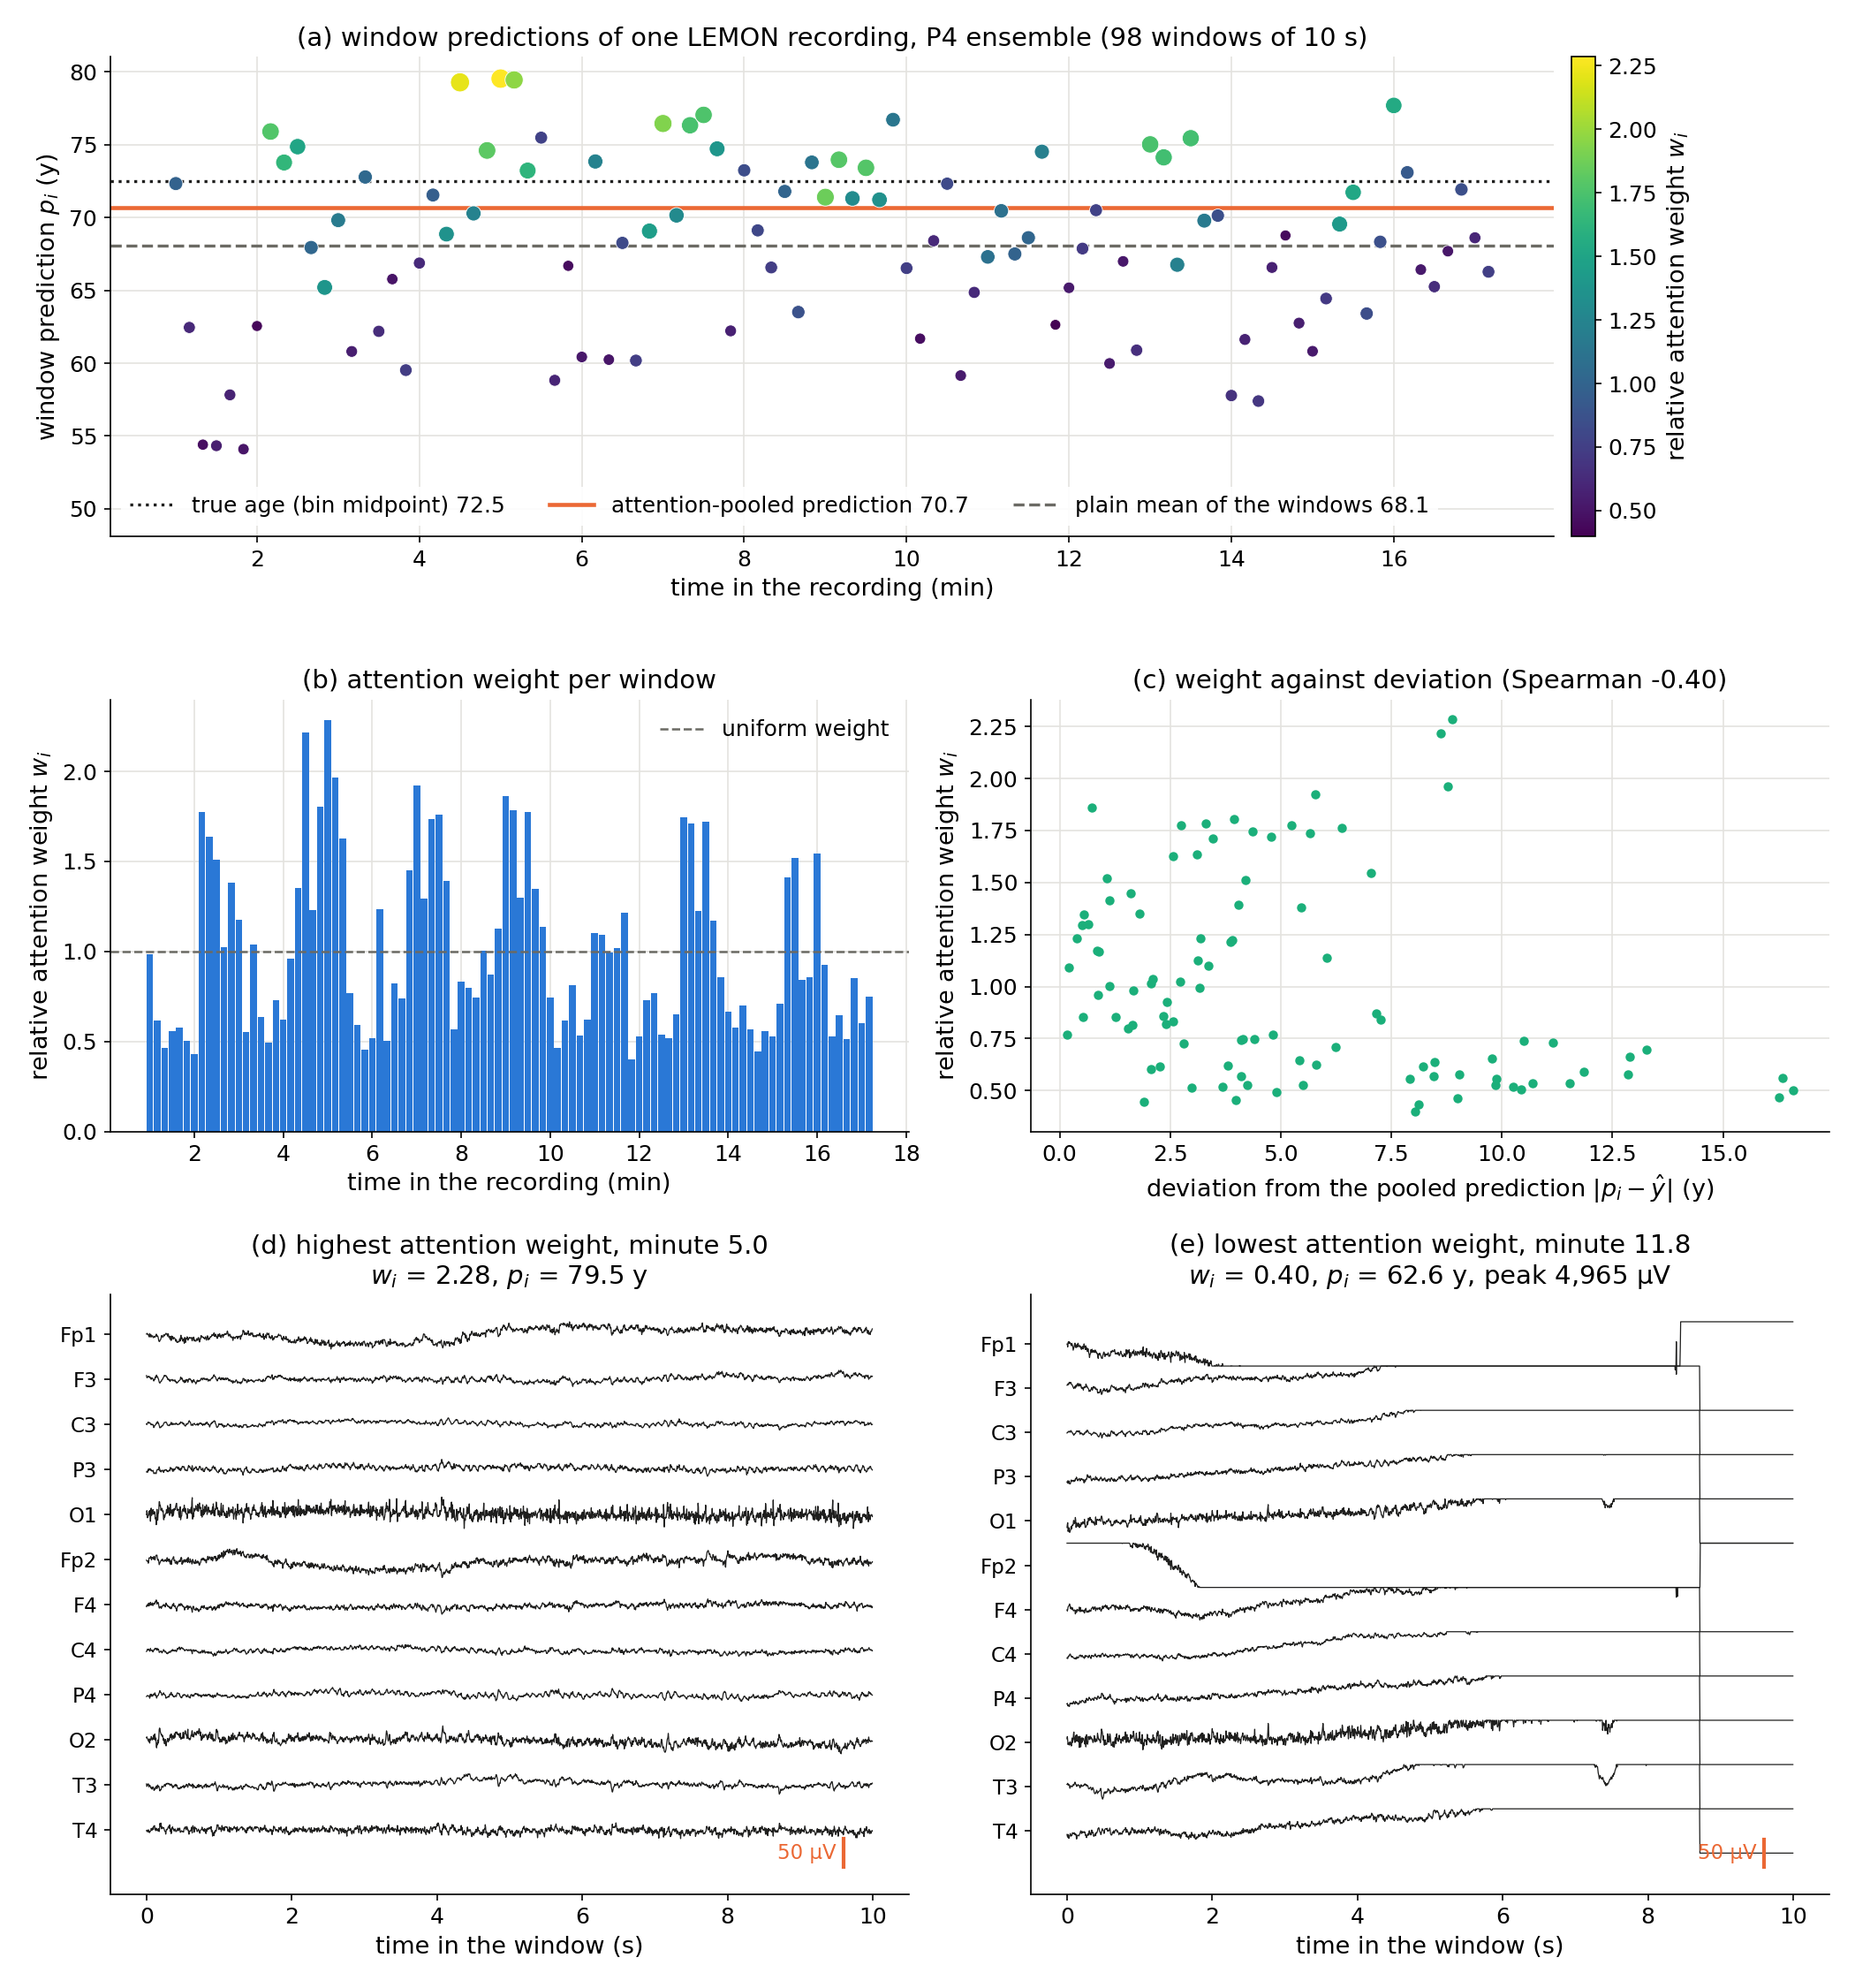
\includegraphics[width=\textwidth,height=0.62\textheight,keepaspectratio]{fig_attention_example.png}
\caption{Attention pooling over the windows of one recording: LEMON participant aged 70--75, 98 windows of 10 s after the 60 s trims, P4 ensemble ($p_i$ and $w_i$ of Eq. (20)). (a) Window predictions over time, coloured and sized by the relative attention weight $w_i$ (1 = uniform); lines: the true age (bin midpoint), the attention-pooled prediction of Eq. (12) and the plain mean of the windows. (b) The weight per window. (c) Weight against the window's deviation from the pooled prediction, Eq. (21). (d), (e) The EEG of the highest- and the lowest-weighted window, 12 of 19 channels after the common average reference, traces 80 $\mu$V apart and clipped at $\pm$40 $\mu$V. The recording was chosen to illustrate the mechanism; over all LEMON recordings attention improves on the plain mean by 0.4 years (Section 6.3). \texttt{scripts/tech\_report\_figures.py}.}
\end{figure}


Figures 8 and 9 show where in a whole recording the attention is placed. Figure 8 draws the EEG itself, with each 10 s window's background coloured by its attention weight: green where the model relies on the window more than average, red where it relies on it less. In the well-predicted recording (Figure 8(a), (b)) the two red windows at 490--510 s hold a movement artifact on every channel (weights 0.58 and 0.25), while windows of calm resting EEG sit near or above the uniform weight; the window predictions there are 60 to 66 years for a person of 60 to 65. In the badly predicted recording (Figure 8(c), (d)) the red windows again hold artifacts, here eye movements and saturated frontal channels, and the green windows are calm. Attention therefore finds the clean signal in both recordings. The difference is what the clean signal says: in the weak case even the most trusted windows read 30 to 33 years for a person of 20 to 25.

Figure 9 shows the same for three recordings as a map over the five fold models. In the good case (Figure 9(a)) the window predictions scatter on both sides of the true age (49 \% above it), and the artifact at minute 8 is a column of near-zero weight in all five fold models. In the two bad cases (Figure 9(b), (c)) every window errs in the same direction as the final answer, 100 \% of them too old or too young. The fold models agree on the weights (mean correlation of their weight maps 0.6 to 0.7, against 0.5 in the good case), but no weighting of uniformly biased windows can reach the true age: attention-pooled and plain-mean predictions differ by about 1 year at most. The error of such a recording lies in what every window looks like to the encoder, not in which windows are chosen, which is why the spread and fold-disagreement scores of Section 4.5, not the attention weights, flag uncertain recordings.

\begin{figure}[t]
\centering
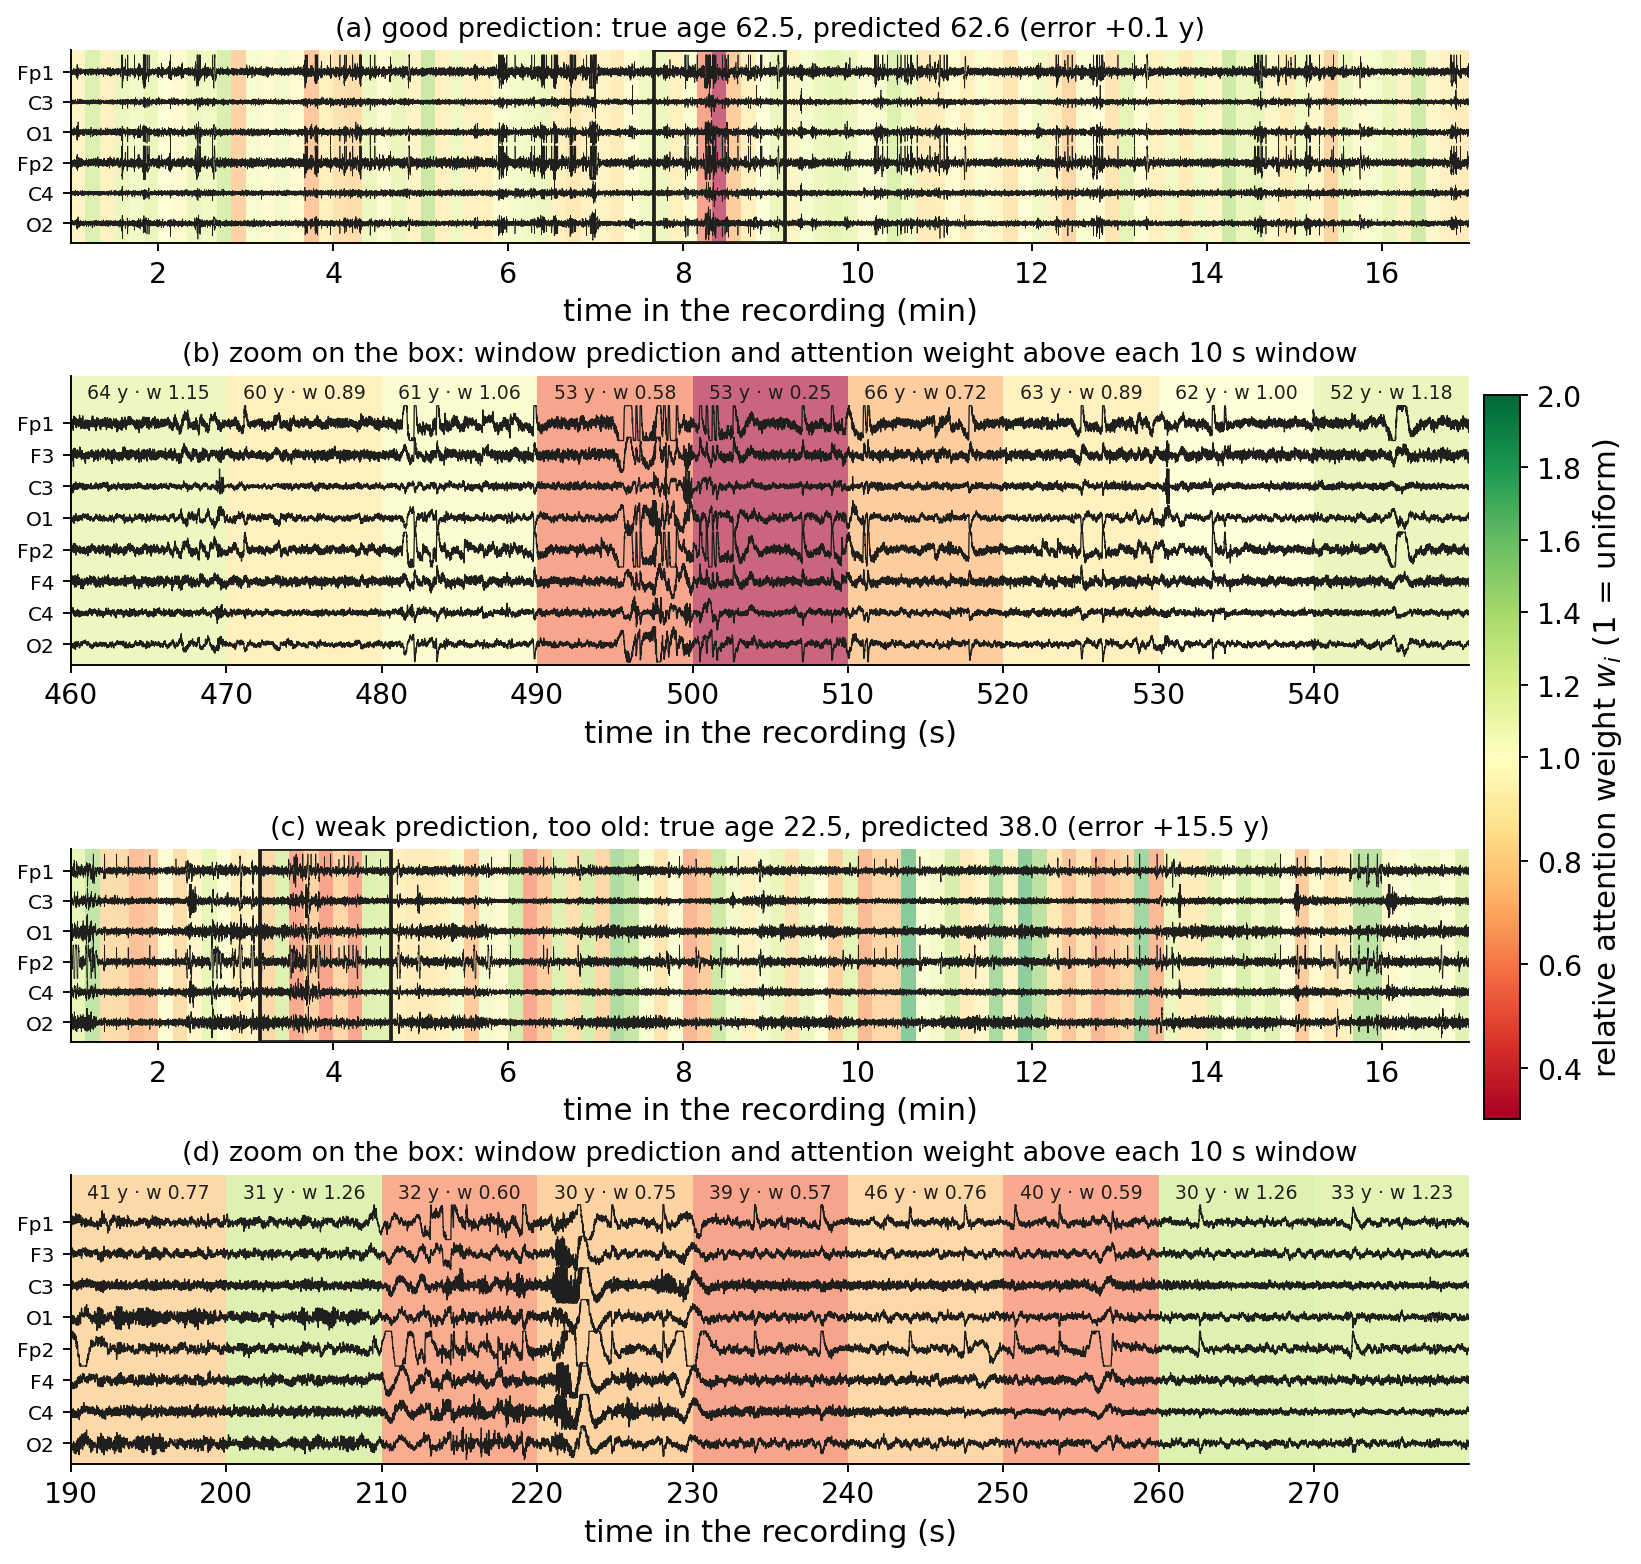
\includegraphics[width=\textwidth,height=0.62\textheight,keepaspectratio]{fig_attention_on_eeg.png}
\caption{Attention on the EEG, P4 ensemble, two LEMON participants: (a), (b) a good prediction (aged 60--65, predicted 62.6), (c), (d) a weak one predicted too old (aged 20--25, predicted 38.0). (a), (c) The whole scored recording (after the 60 s trims), 6 channels; (b), (d) the 90 s in the box, 8 channels, with each window's prediction (fold mean) and relative attention weight $w$ above it. Background: the window's mean relative attention weight over the five fold models (Eq. (20); 1 = uniform, red below, green above). Display only: common average reference, 0.5 Hz high-pass, traces clipped. \texttt{scripts/tech\_report\_figures.py}.}
\end{figure}


\begin{figure}[t]
\centering
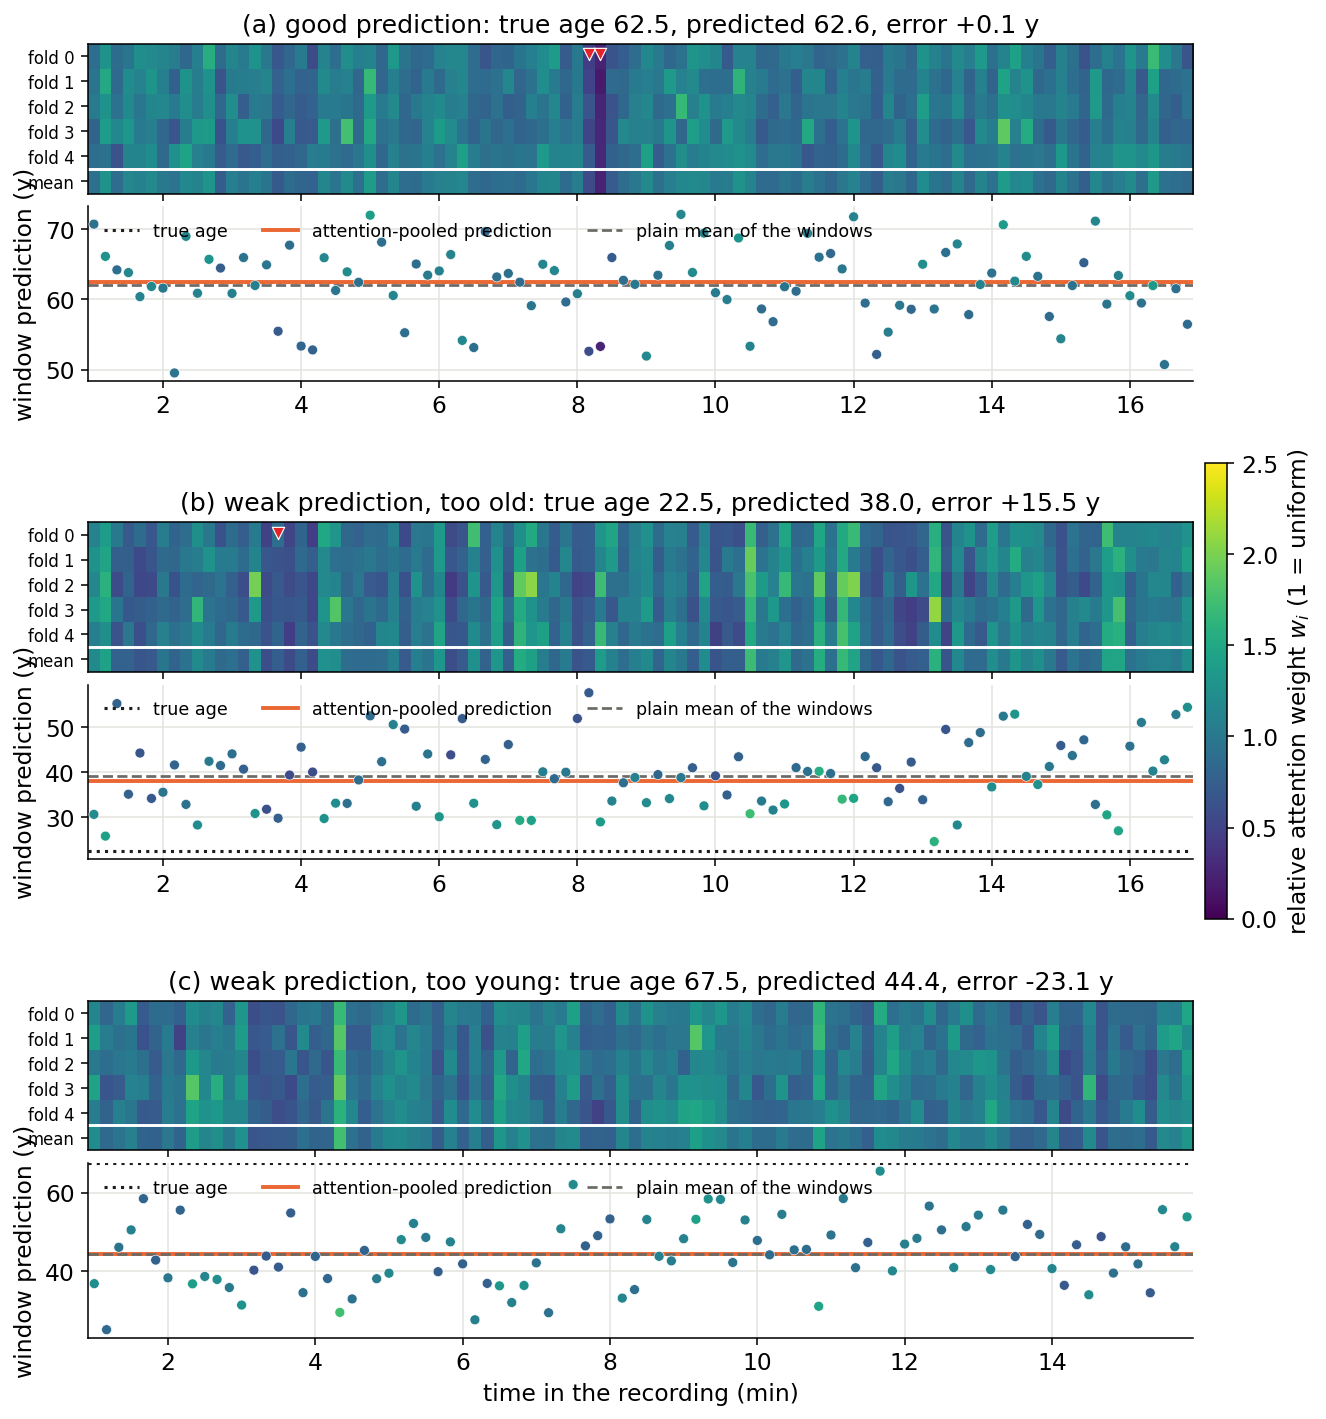
\includegraphics[width=\textwidth,height=0.62\textheight,keepaspectratio]{fig_attention_heatmaps.png}
\caption{Attention over whole recordings as a map over the fold models, P4 ensemble, three LEMON participants: (a) a good prediction (aged 60--65, predicted 62.6), (b) a weak one predicted too old (aged 20--25, predicted 38.0), (c) a weak one predicted too young (aged 65--70, predicted 44.4). For each, top: the relative attention weight $w$ of every 10 s window (1 = uniform; colour scale shared) for each of the five fold models and their mean; middle: the window predictions (fold means, coloured by the mean weight), the true age (bin midpoint), the attention-pooled prediction of Eq. (12) and the plain mean of the windows. Red markers: windows whose median channel standard deviation after the common average reference exceeds 100 $\mu$V (artifacts). Recordings after the 60 s trims. Chosen to illustrate the extremes: the median absolute error on LEMON is 3.3 years. \texttt{scripts/tech\_report\_figures.py}.}
\end{figure}


Training is one run of 17 epochs from the pre-trained encoder, in three phases (Table 11). The two recipes differ in the schedule and in the regulariser of the joint phase: P3 restarts the learning rate and uses retention; P4 keeps one cosine schedule and adds the per-window loss.

\begin{table}[t]
\centering
\small
\caption{The phased recipes. Batches are 32 recordings $\times$ 8 windows; peak learning rate $2.8 \times 10^{-4}$; the pool and the head use a 5 times higher learning rate from the attention-only phase on.}
\begin{tabular}{llll}
\toprule
\textbf{phase} & \textbf{what trains} & \textbf{P3} & \textbf{P4} \\
\midrule
window & encoder and head, window loss of Eq. (7) & epochs 0--9, own cosine schedule ending near 0 & epochs 0--7 \\
attention only & the pool; encoder and head frozen & epoch 10, warm-up to $10^{-4}$ & epoch 8 \\
joint & pool, encoder and head, Eq. (11) & epochs 11--16, cosine from $10^{-4}$; $\lambda_{ret} = 0.1$, $\lambda_w = 0$ & epochs 9--16 on one cosine over all 17 epochs; $\lambda_w = 0.5$, $\lambda_{ret} = 0$; every recording drawn twice per epoch \\
\bottomrule
\end{tabular}
\end{table}


\subsection{Cross-validation ensemble}

The training and validation patients are divided into five folds, no patient in two folds. Fold model $k$ validates on fold $k$, which selects its best epoch, and trains on the other four. The test split is the same for every fold and is never seen. The ensemble prediction is the mean of the five fold models~\citep{lakshminarayanan2017ensembles}:

\begin{equation}
\hat y_r = \frac{1}{5} \sum_{k=1}^{5} \hat y_{r,k} \tag{12}
\end{equation}

Figure 10 follows the three one-run recipes through their training, as the mean and standard deviation over the five fold models of each recipe (\texttt{docs/data/mil\_phased\_cv/cv\_curves.csv}). In the window phase (blue background) the encoder and head learn per window and the validation error falls from about 9.5 to 7.5 years. The attention-only phase (yellow), one or two epochs in which only the new attention pool trains, gives the largest single step: the validation error drops by 0.6 to 0.7 years (P3 7.52 to 6.95, P4 7.73 to 7.07). The joint phase (purple) adds another 0.4 to 0.5 years and flattens from about epoch 13. The training-sample error keeps falling to the end (P4 3.63 years) while validation and test stay flat, so the gap between them, the over-fitting, grows with the number of joint epochs: 1.57 years for P1 (4 joint epochs), 2.33 for P3 and 2.96 for P4, with almost the same final validation error (6.59 to 6.60) and test error (6.09 to 6.16 per fold model). The five fold models agree closely: at the last epoch their standard deviation is 0.06 to 0.07 years on validation and 0.01 to 0.03 on test.

\begin{figure}[t]
\centering
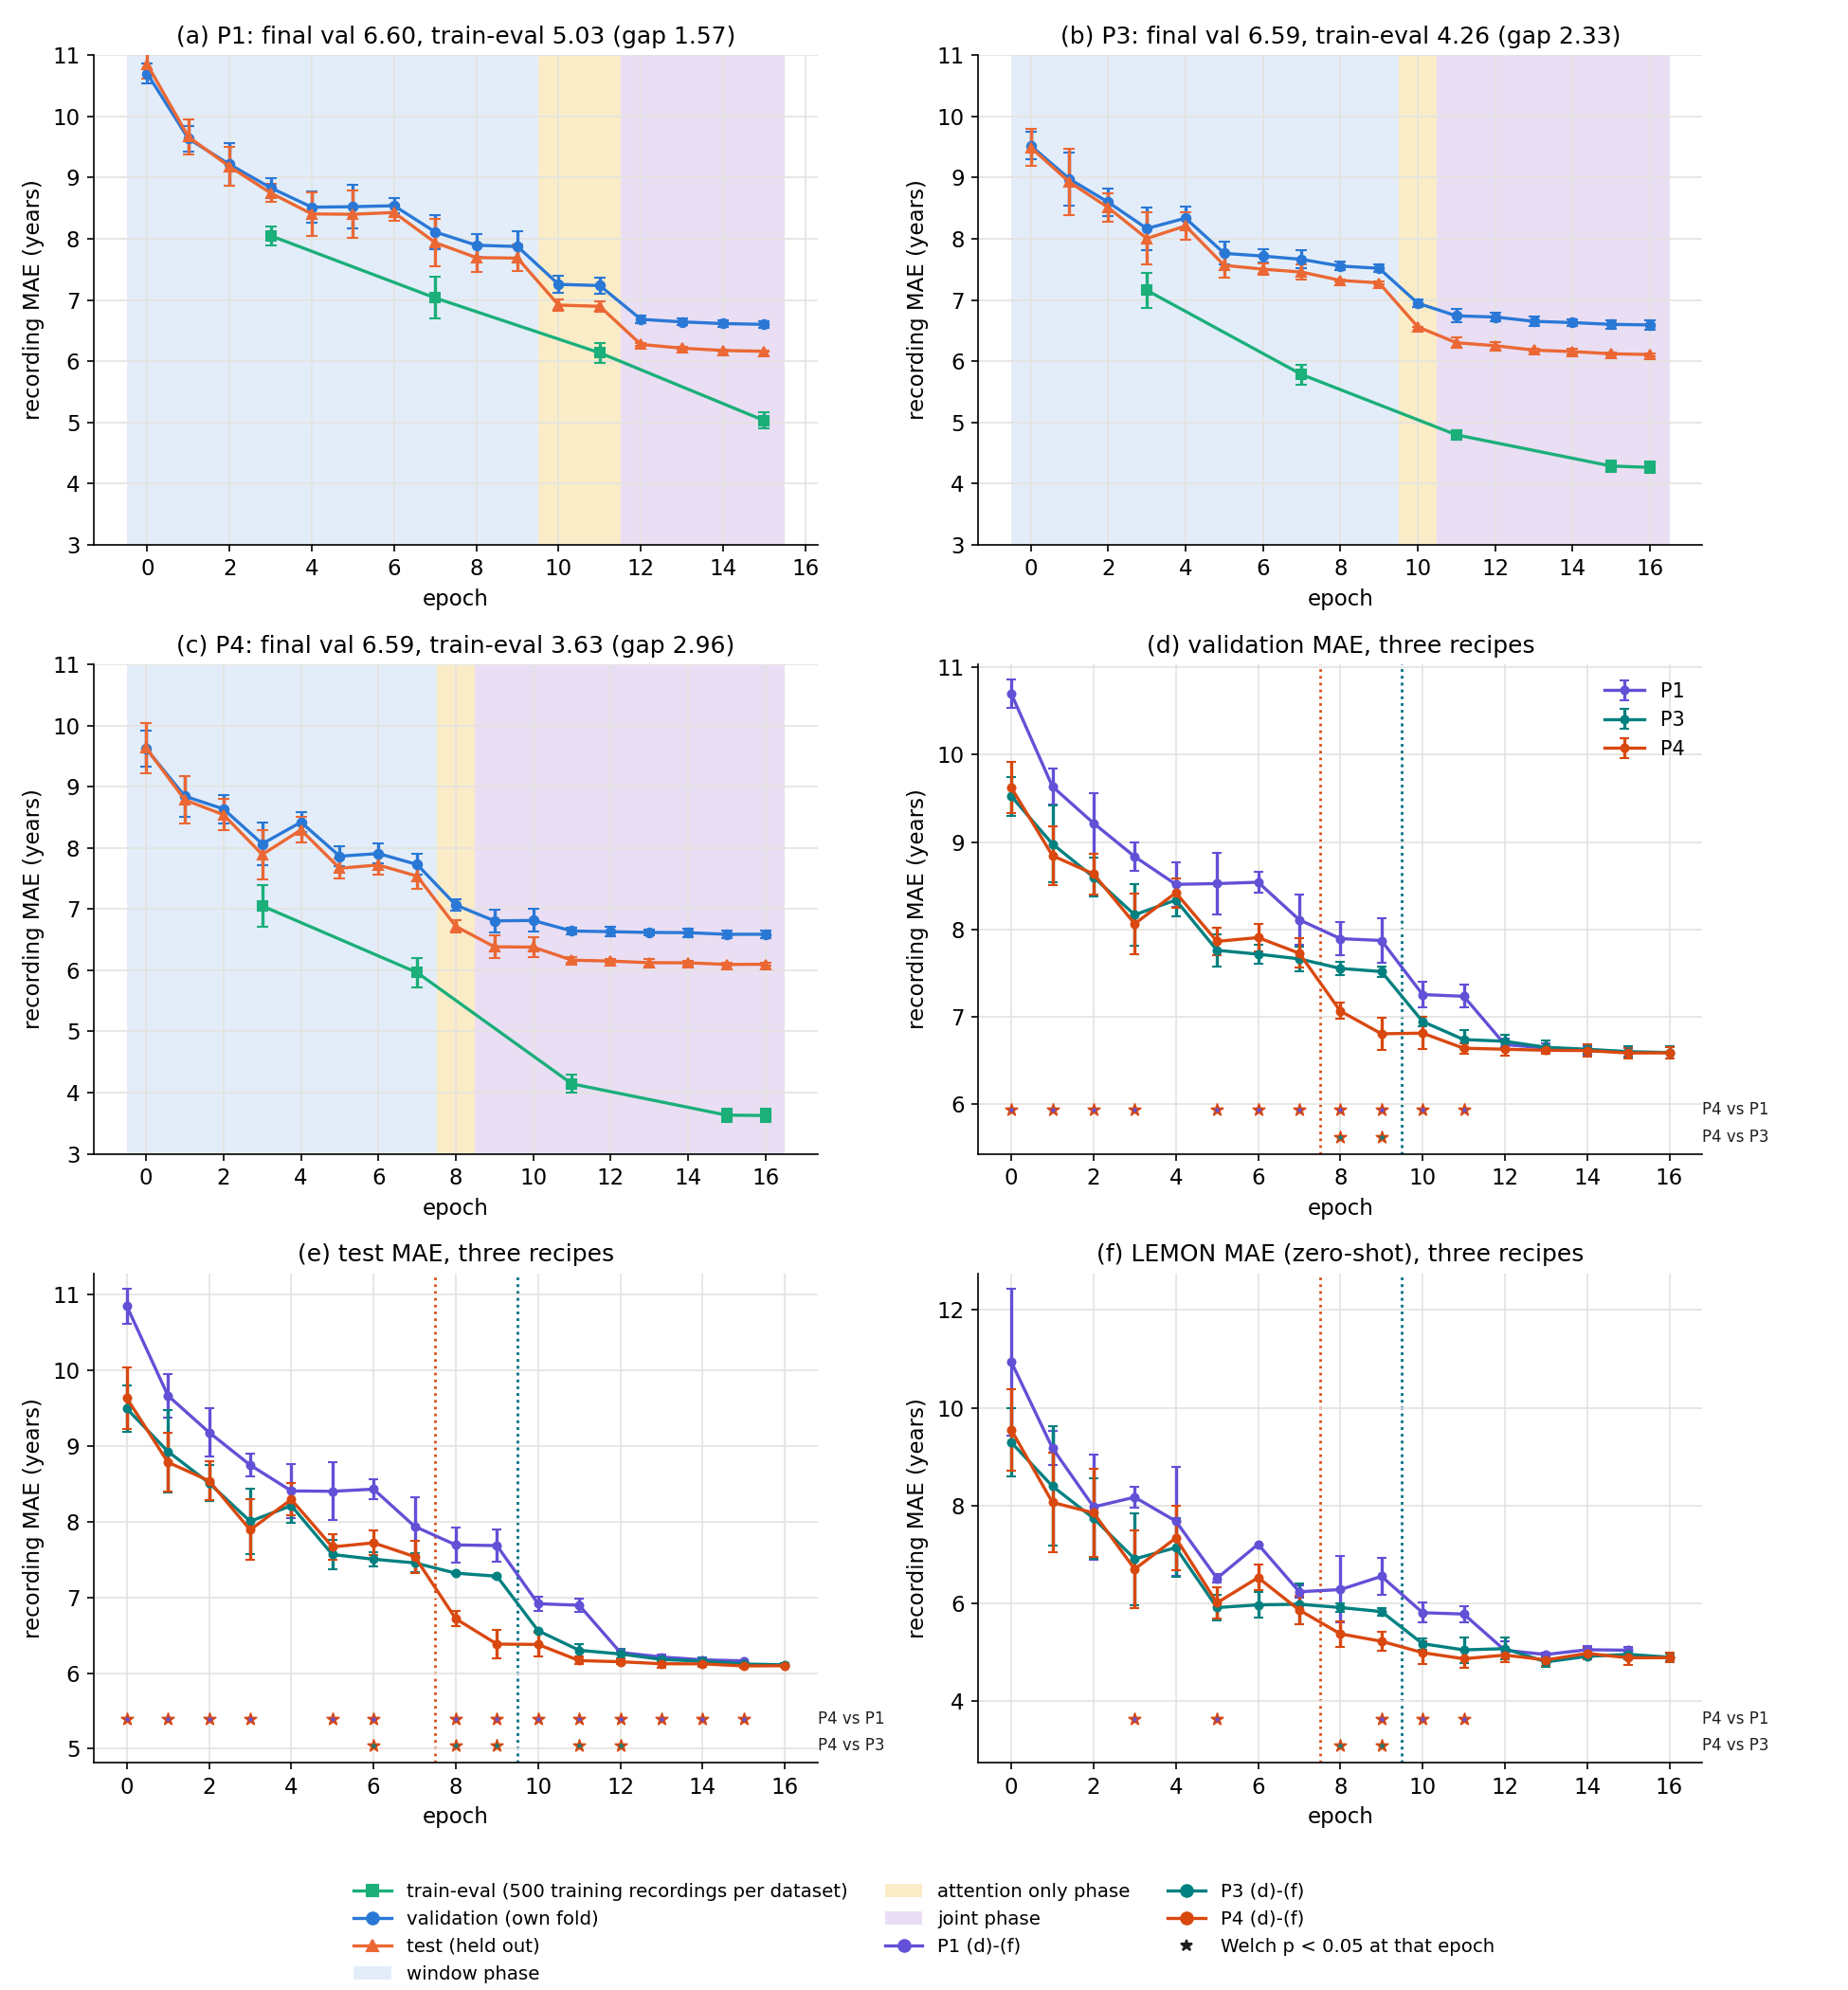
\includegraphics[width=\textwidth,height=0.62\textheight,keepaspectratio]{fig_cv_curves.png}
\caption{Cross-validation of the one-run recipes over epochs: recording MAE in years, mean over the five fold models with the sample standard deviation as error bar, for (a) P1 (10 window, 2 attention-only, 4 joint epochs), (b) P3 and (c) P4 (Table 11). Train-eval: a fixed sample of 500 training recordings per dataset, scored every 4 epochs like validation; validation: each fold model's own validation fold; test: the held-out test split. Background: the training phase. Training on Temple + Harvard; first 5 minutes of every scored recording. \texttt{scripts/tech\_report\_figures.py}.}
\end{figure}


Figure 11 compares the three recipes epoch by epoch. P4, whose attention-only phase comes two epochs earlier, is significantly better than P3 at epochs 8 and 9 on validation and LEMON (and also at 6, 11 and 12 on test), and better than P1 through most of training; from about epoch 13 the three recipes converge to the same validation and test error.

\begin{figure}[t]
\centering
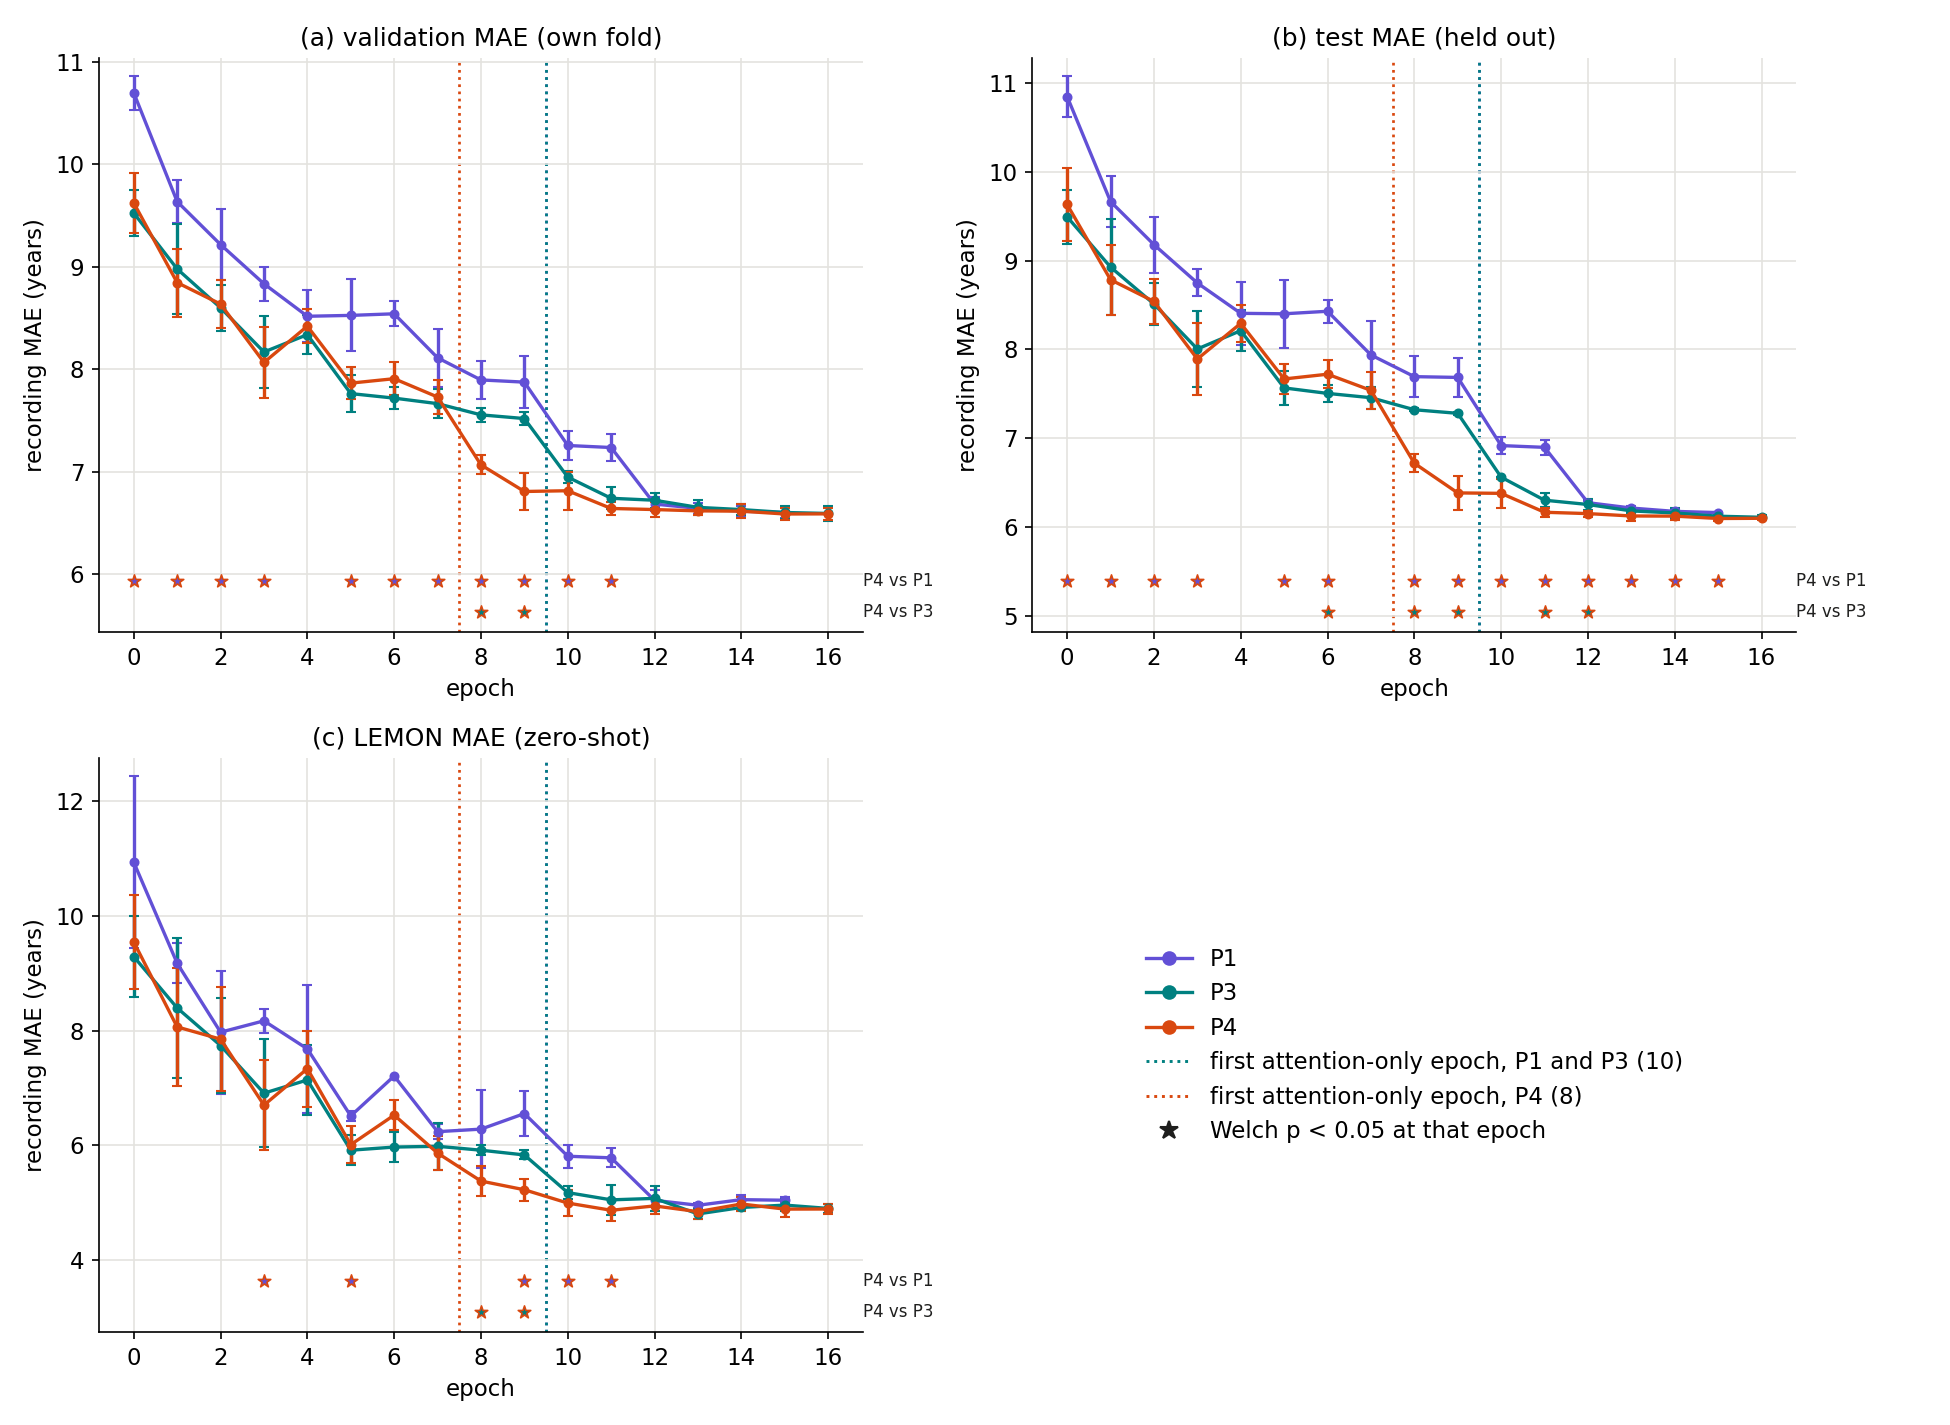
\includegraphics[width=\textwidth,height=0.62\textheight,keepaspectratio]{fig_cv_compare.png}
\caption{The three one-run recipes compared over epochs: (a) validation MAE (each fold model's own fold), (b) test MAE (held out), (c) LEMON MAE (zero-shot), fold mean $\pm$ standard deviation, in years. Dotted lines: the first attention-only epoch of each recipe. Stars: epochs at which P4 differs from P3 or from P1, $p < 0.05$ in a two-sided Welch $t$-test computed from the two recipes' fold means, standard deviations and $n = 5$ (it measures the spread between fold models, not the sampling of the test recordings). \texttt{scripts/tech\_report\_figures.py}.}
\end{figure}


Figure 12 splits the test curves of Figure 11(b) by data cohort. The order of the recipes is the same in every cohort: P4 leads from its earlier attention phase (epoch 8) to about epoch 12, P1 trails until its joint phase, and at the last epoch the three recipes are within 0.07 to 0.15 years of each other in every cohort. No difference between P4 and P3 is significant after epoch 13 in any cohort (after epoch 12 over all test recordings); P1 stays about 0.1 years behind on the Harvard normal and no-report recordings, small but consistent across its fold models (significant up to its last epoch). The abnormal-report recordings carry the largest fold-to-fold spread (Temple $\pm$0.3 years at the end), the Harvard cohorts the smallest.

\begin{figure}[t]
\centering
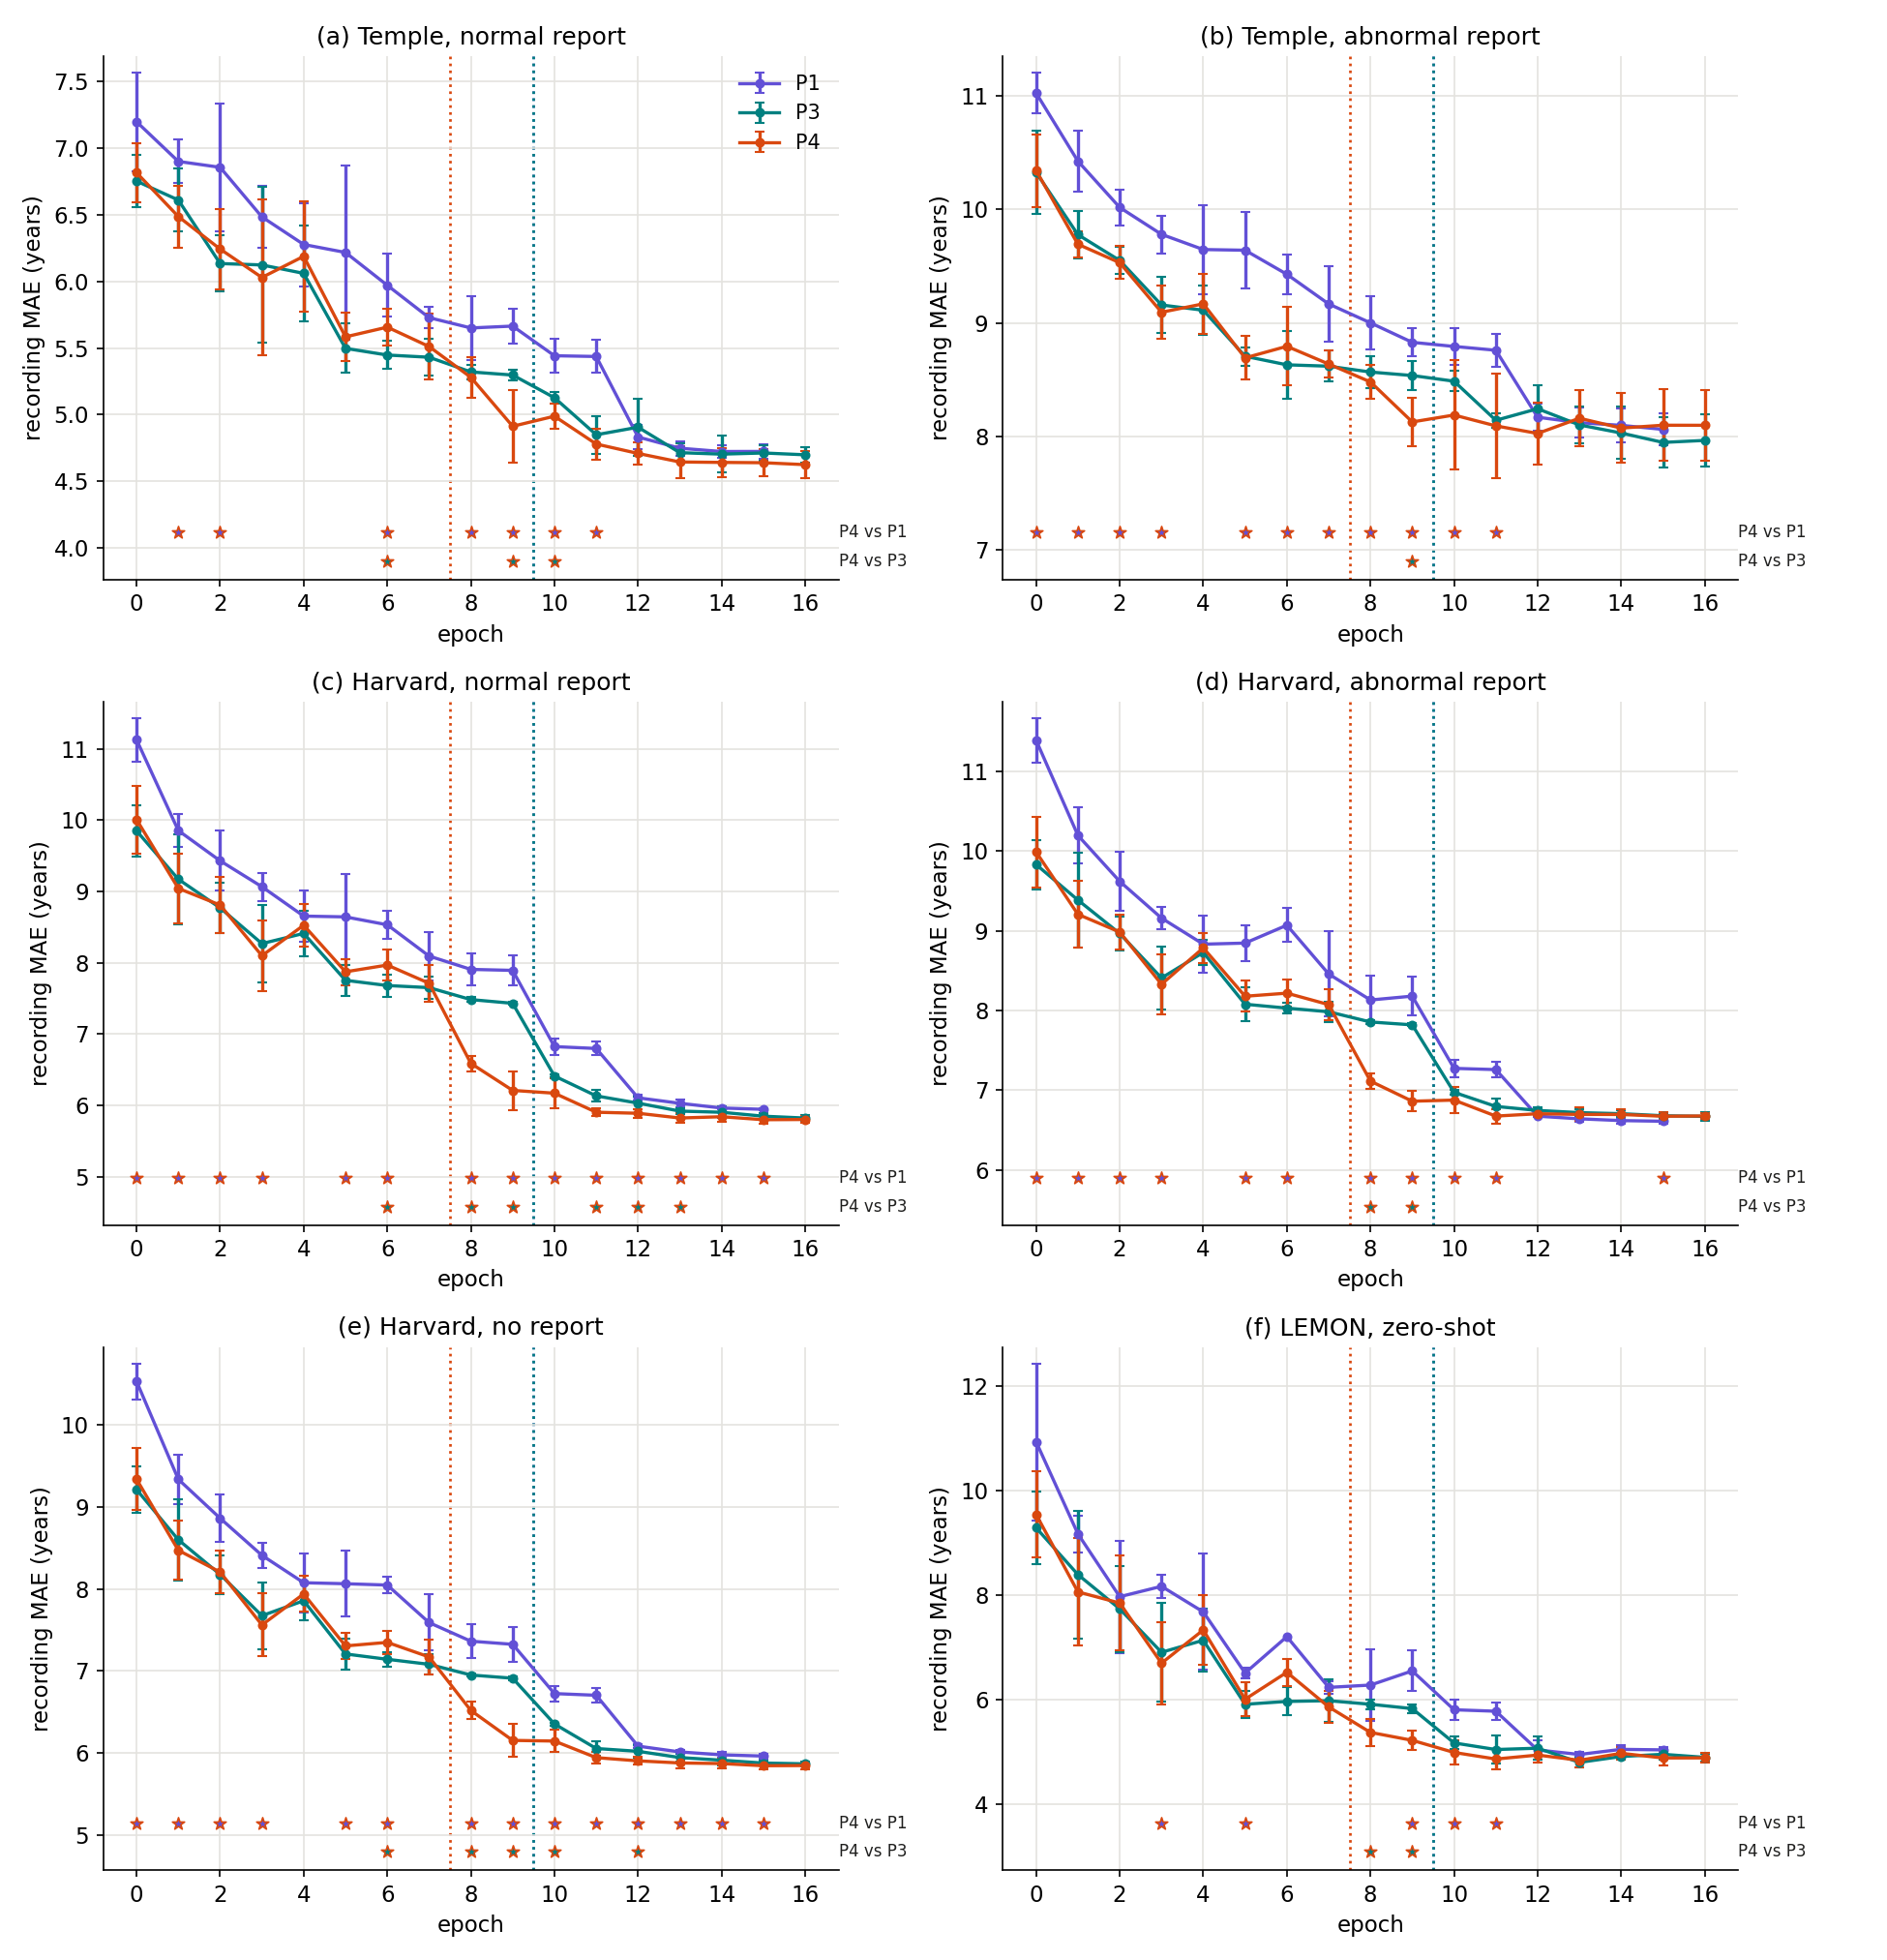
\includegraphics[width=\textwidth,height=0.62\textheight,keepaspectratio]{fig_cv_cohorts.png}
\caption{Held-out test MAE per data cohort over epochs, the three one-run recipes (fold mean $\pm$ standard deviation): (a) Temple, normal report (149 recordings), (b) Temple, abnormal report (125), (c) Harvard, normal report (1,518), (d) Harvard, abnormal report (2,253), (e) Harvard, no report (3,567), (f) LEMON, zero-shot (214). Dotted lines and stars as in Figure 11.}
\end{figure}


\subsection{Confidence and selective prediction}

For fold model $k$, with window predictions $p_i = \mu_k + \sigma_k \, g(h_{r,i})$ and attention weights $\alpha_i$, the within-recording spread and the standard error of the pooled prediction are

\begin{equation}
s_{r,k} = \sqrt{ \sum_i \alpha_i \, (p_i - \hat y_{r,k})^2 }, \qquad e_{r,k} = s_{r,k} \sqrt{ \sum_i \alpha_i^2 } \tag{13}
\end{equation}

The disagreement of the fold models and a combined uncertainty are

\begin{equation}
d_r = \operatorname{sd}_k\big( \hat y_{r,k} \big), \qquad u_r = \sqrt{ \frac{1}{5}\sum_{k} e_{r,k}^2 + d_r^2 } \tag{14}
\end{equation}

We compare three rejection scores: \textbf{spread}, the fold mean of $s_{r,k}$ (for the single model E2L, the plain standard deviation of its window predictions); \textbf{total}, $u_r$; and \textbf{learned}, a gradient-boosted regressor of the absolute error on the window scores and the predicted age, fitted on each fold model's own validation fold and rank-averaged with $d_r$. None uses the age of a scored recording. In selective prediction~\citep{geifman2017selective} the fraction $1 - c$ of a cohort with the highest score gets no prediction, and the risk at coverage $c$ is the MAE of the rest:

\begin{equation}
\mathrm{MAE}(c) = \frac{1}{\lvert S_c \rvert} \sum_{r \in S_c} \lvert \hat y_r - y_r \rvert, \qquad S_c = \{\, r : \text{score}_r \le q_c \,\} \tag{15}
\end{equation}

where $q_c$ is the $c$-quantile of the score in the cohort.

\subsection{Age-bias correction}

Brain-age models predict toward the mean age: the gap $\hat y - y$ falls with age~\citep{smith2019delta}. On validation recordings with a normal EEG report we fit by least squares

\begin{equation}
\hat y \approx a\,y + b, \qquad y \approx c\,\hat y + d, \qquad \hat y - y \approx c_0 + c_1 y + c_2 y^2 \tag{16}
\end{equation}

and compare four corrections. Two need no true age and give a new age estimate, the inversion of Cole et al.~\citep{cole2018mortality} and a recalibration:

\begin{equation}
\hat y^{cole} = \frac{\hat y - b}{a}, \qquad \hat y^{recal} = c\,\hat y + d \tag{17}
\end{equation}

Two remove the age trend of the gap using the true age~\citep{beheshti2019bias,delange2020commentary}, linearly or quadratically as in Gemein et al.~\citep{gemein2024revisited}:

\begin{equation}
\hat y^{lin} = \hat y - \big( (a-1)\,y + b \big), \qquad \hat y^{quad} = \hat y - \big( c_0 + c_1 y + c_2 y^2 \big) \tag{18}
\end{equation}

Eq. (18) gives a corrected gap for group comparisons, not a deployable age estimate. Section 10.1 gives the fit, the fitted coefficients and the consequences of using the true age.

\subsection{Metrics}

For a group of $N$ recordings we report the MAE, the mean gap (bias), the Pearson correlation $r$ of $\hat y$ and $y$, and

\begin{equation}
\mathrm{MAE} = \frac{1}{N} \sum_r \lvert \hat y_r - y_r \rvert, \qquad R^2 = 1 - \frac{\sum_r (\hat y_r - y_r)^2}{\sum_r (y_r - \bar y)^2} \tag{19}
\end{equation}

with $\bar y$ the group's own mean age, so that $R^2 \le 0$ means no better than predicting that mean. Intervals are 95 \% percentile intervals over 2,000 bootstrap resamples of subjects. In-domain cohorts are scored on the first 5 minutes after the trim, the training protocol; external cohorts on every window. A TDBRAIN or Dortmund session is the mean of the predictions of its runs. Section 10.4 scores every cohort on one fixed window instead.

\subsection{Window-level diagnostics and group comparisons}

To see what the confidence measures at the level of a window, we compare, for window $i$ of a recording with $n$ scored windows, its error with three label-free quantities of the ensemble:

\begin{equation}
p_i = \frac{1}{5}\sum_k p_{ik}, \qquad e_i = \lvert p_i - y_r \rvert, \qquad w_i = \frac{n}{5}\sum_k \alpha_{ik} \tag{20}
\end{equation}

\begin{equation}
d_i = \lvert p_i - \hat y_r \rvert, \qquad s_i = \operatorname{sd}_k\big( p_{ik} \big) \tag{21}
\end{equation}

$e_i$ is the window error, $w_i$ the relative attention weight (1 is the uniform weight), $d_i$ the deviation of the window from the recording's prediction (its share of the spread of Eq. (13)) and $s_i$ the disagreement of the fold models on the window.

A clinical group $G$ is compared with a reference group through the gap $g_r = \hat y_r - y_r$. With $x_r = 1$ for the recordings of $G$ and 0 for the reference, we fit

\begin{equation}
g_r = \beta\,x_r + c_{b(r)} + \gamma_1\,y_r + \gamma_2\,m_r + \varepsilon_r \tag{22}
\end{equation}

where $c_b$ is one intercept per 5-year age band, $m_r$ is 1 for men, and the standard error of $\beta$ is clustered by patient. $\beta$ is how much older the group looks at the same age and sex. The age terms take the place of the corrections of Eq. (18), as recommended when the gap is compared between groups~\citep{delange2020commentary}. The same model with $\lvert g_r \rvert$ on the left gives the group's extra absolute error. P-values over several groups are adjusted for the false discovery rate~\citep{benjamini1995fdr}.

\section{What we learned on the way}

Table 12 collects the steps from the classical recipe to the present models, each with its measured effect. Early steps were measured on the TUAB test set (274 recordings), later ones on the test split of \texttt{tuh\_heedb\_v1} (7,612 recordings).

\begin{table}[t]
\centering
\small
\caption{Ablations. MAE in years; "n.s." means within the run-to-run noise (seed standard deviation 0.14 years on TUAB).}
\begin{tabular}{lll}
\toprule
\textbf{change} & \textbf{measured on} & \textbf{MAE before $\rightarrow$ after} \\
\midrule
common average reference at the input & TUAB test & 8.91 $\rightarrow$ 8.30 \\
pre-trained encoder instead of training from scratch & TUAB test & 9.42 $\rightarrow$ 8.30 \\
more data: TUAB (2,145 recordings) $\rightarrow$ full Temple (about 20,000) $\rightarrow$ Temple + Harvard & TUAB test & 8.23 $\rightarrow$ 7.26 $\rightarrow$ 6.70 \\
longer training on Temple + Harvard (8 $\rightarrow$ 16 epochs, E2L) & Temple + Harvard test & 7.25 $\rightarrow$ 7.00 \\
60 Hz line removal for Temple (US mains) & TUAB test & $-$0.23 \\
recording-level loss with attention pooling (two-step, from E2L) & Temple + Harvard test & 7.00 $\rightarrow$ 6.09 \\
one phased run from the pre-trained encoder (P3, P4) instead of two steps & Temple + Harvard test & 6.09 $\rightarrow$ 6.11 / 6.09 (5-fold mean), at 12.5 vs 27.7 GPU hours \\
5-fold ensemble instead of one fold model & Temple + Harvard test & P3 6.11 $\rightarrow$ 5.98; P4 6.09 $\rightarrow$ 5.94 \\
scoring every window instead of the first 5 minutes & Temple + Harvard test & 6.09 $\rightarrow$ 5.46 (two-step model) \\
band-limited (1--45 Hz), amplitude-normalised input (device-robust E2L, Section 6.5) & CHBP / Temple + Harvard test & 9.35 $\rightarrow$ 5.90 / 7.00 $\rightarrow$ 7.55 \\
\bottomrule
\end{tabular}
\end{table}


What the ablations show:

\begin{itemize}
\item \textbf{Data and the training objective matter most.} Going from 2,145 to about 100,000 training recordings is worth 1.5 years on the same test set, and the recording-level objective another 0.9 years. In a controlled comparison from the pre-trained encoder at equal budget, the window model reaches 7.64, a bag with mean pooling 6.98 and a bag with attention 6.69: about 70 \% of the gain comes from the recording-level loss and 30 \% from attention.
\item \textbf{The small corpus is memorised.} On TUAB alone the training MAE falls from 7.2 to 1.2 years while the validation MAE stays at 7.8. Of 51 changes tested on TUAB, 7 improved, 7 hurt and 37 were within noise.
\item \textbf{What did not help:} an L1 loss (+0.41), longer windows of 30 s (+0.44), low-rank adaptation of the encoder (+0.99), classical features as extra tokens (+0.76), other heads, a multi-task normal / abnormal head, window-quality rejection and artifact-aware pooling (all n.s.). Dropout of 0.1 in the encoder made the model collapse. Mixup alone is not significant on TUAB and is kept as a regulariser.
\item \textbf{Longer bag training does not help.} 20 joint epochs tie 4; only the retention term lowered the gap between training and validation error.
\item \textbf{Robustness to the recording chain costs in-domain accuracy.} The band-limited, amplitude-normalised model fixes CHBP but loses 0.55 years in-domain and 0.9 years on LEMON (5.20 $\rightarrow$ 6.07), so it is not a free default (Section 6.5).
\end{itemize}

\section{Results}

\subsection{Accuracy on seven cohorts}

\begin{table}[t]
\centering
\small
\caption{MAE in years and, in brackets, $R^2$, by cohort and subset. Adults; \texttt{n}: recordings (TDBRAIN and Dortmund: sessions); subsets by EEG report (Temple, Harvard) or clinical group (TDBRAIN); the research cohorts hold healthy volunteers only. $R^2$ uses each row's own mean age, so it is low for subsets with a narrow age range. Models: the window model E2L; two attention models trained in two steps from E2L's checkpoint (4 bag epochs, \texttt{docs/mil\_stage1\_results.md}), L1 with the attention pool of Eq. (10) and W4 with a gated attention pool~\citep{ilse2018abmil}; and the one-run attention ensembles P3 and P4 (Section 4). Bold: the best model of the row (ties bold). 95 \% intervals are in Tables 35 to 41; best published values with their protocol in the last column (Section 7).}
\resizebox{\textwidth}{!}{%
\begin{tabular}{lllllllll}
\toprule
\textbf{cohort} & \textbf{subset} & \textbf{n} & \textbf{E2L} & \textbf{L1} & \textbf{W4} & \textbf{P3 ens.} & \textbf{P4 ens.} & \textbf{best published} \\
\midrule
Temple, in-domain & all & 272 & 6.40 (0.78) & 6.01 (0.79) & 6.05 (0.79) & \textbf{5.87} (0.81) & \textbf{5.87} (0.81) &  \\
 & normal report & 149 & 4.91 (0.85) & \textbf{4.41} (0.88) & 4.45 (0.88) & 4.61 (0.87) & 4.52 (0.87) & 6.60, trained on TUAB normals~\citep{gemein2024revisited} \\
 & abnormal report & 123 & 8.21 (0.62) & 7.94 (0.62) & 7.98 (0.61) & \textbf{7.39} (0.67) & 7.50 (0.67) & 12.85, model trained on TUAB normals~\citep{gemein2024revisited} \\
Harvard, in-domain & all & 7,338 & 7.02 (0.79) & 6.09 (0.83) & 6.10 (0.83) & 5.98 (0.84) & \textbf{5.94} (0.84) & none found \\
 & normal report & 1,518 & 7.12 (0.78) & 5.71 (0.83) & 5.72 (0.83) & 5.73 (0.84) & \textbf{5.69} (0.84) &  \\
 & abnormal report & 2,253 & 7.56 (0.75) & 6.79 (0.78) & 6.77 (0.78) & 6.52 (0.80) & \textbf{6.49} (0.80) &  \\
 & no report & 3,567 & 6.64 (0.81) & 5.80 (0.84) & 5.83 (0.84) & 5.74 (0.85) & \textbf{5.70} (0.85) &  \\
TDBRAIN, zero-shot & all & 1,113 & 5.32 (0.80) & 5.35 (0.80) & 5.34 (0.80) & 5.14 (0.82) & \textbf{4.92} (0.83) & 5.96 trained on TDBRAIN~\citep{khayretdinova2022tdbrain}; 8.36 zero-shot~\citep{hajhassani2026artifact} \\
 & healthy controls & 179 & 5.28 (0.81) & 5.40 (0.78) & 5.57 (0.76) & 5.15 (0.81) & \textbf{4.96} (0.82) &  \\
 & patients & 934 & 5.33 (0.80) & 5.34 (0.80) & 5.29 (0.80) & 5.14 (0.81) & \textbf{4.92} (0.83) &  \\
LEMON, zero-shot & all, healthy & 214 & 5.20 (0.88) & 4.56 (0.91) & \textbf{4.51} (0.91) & 4.70 (0.90) & 4.67 (0.90) & 7.75 trained on LEMON~\citep{engemann2022benchmark}; 9.91 zero-shot~\citep{hajhassani2026artifact} \\
Dortmund, zero-shot & all, healthy & 816 & 5.01 (0.81) & 4.87 (0.82) & 4.92 (0.82) & 4.72 (0.83) & \textbf{4.53} (0.85) & 2.24 trained on Dortmund, abstract only~\citep{azami2025dortmund} \\
SRM, zero-shot & all, healthy & 152 & 5.01 (0.77) & 5.23 (0.74) & 5.23 (0.74) & \textbf{4.75} (0.79) & 4.84 (0.79) & none found \\
CHBP, zero-shot & all, healthy & 250 & 9.35 ($-$0.64) & 9.11 ($-$0.60) & 8.92 ($-$0.52) & \textbf{7.37} ($-$0.14) & 7.95 ($-$0.28) & 6.48 trained on CHBP~\citep{engemann2022benchmark} \\
\bottomrule
\end{tabular}
}
\end{table}


\begin{figure}[t]
\centering
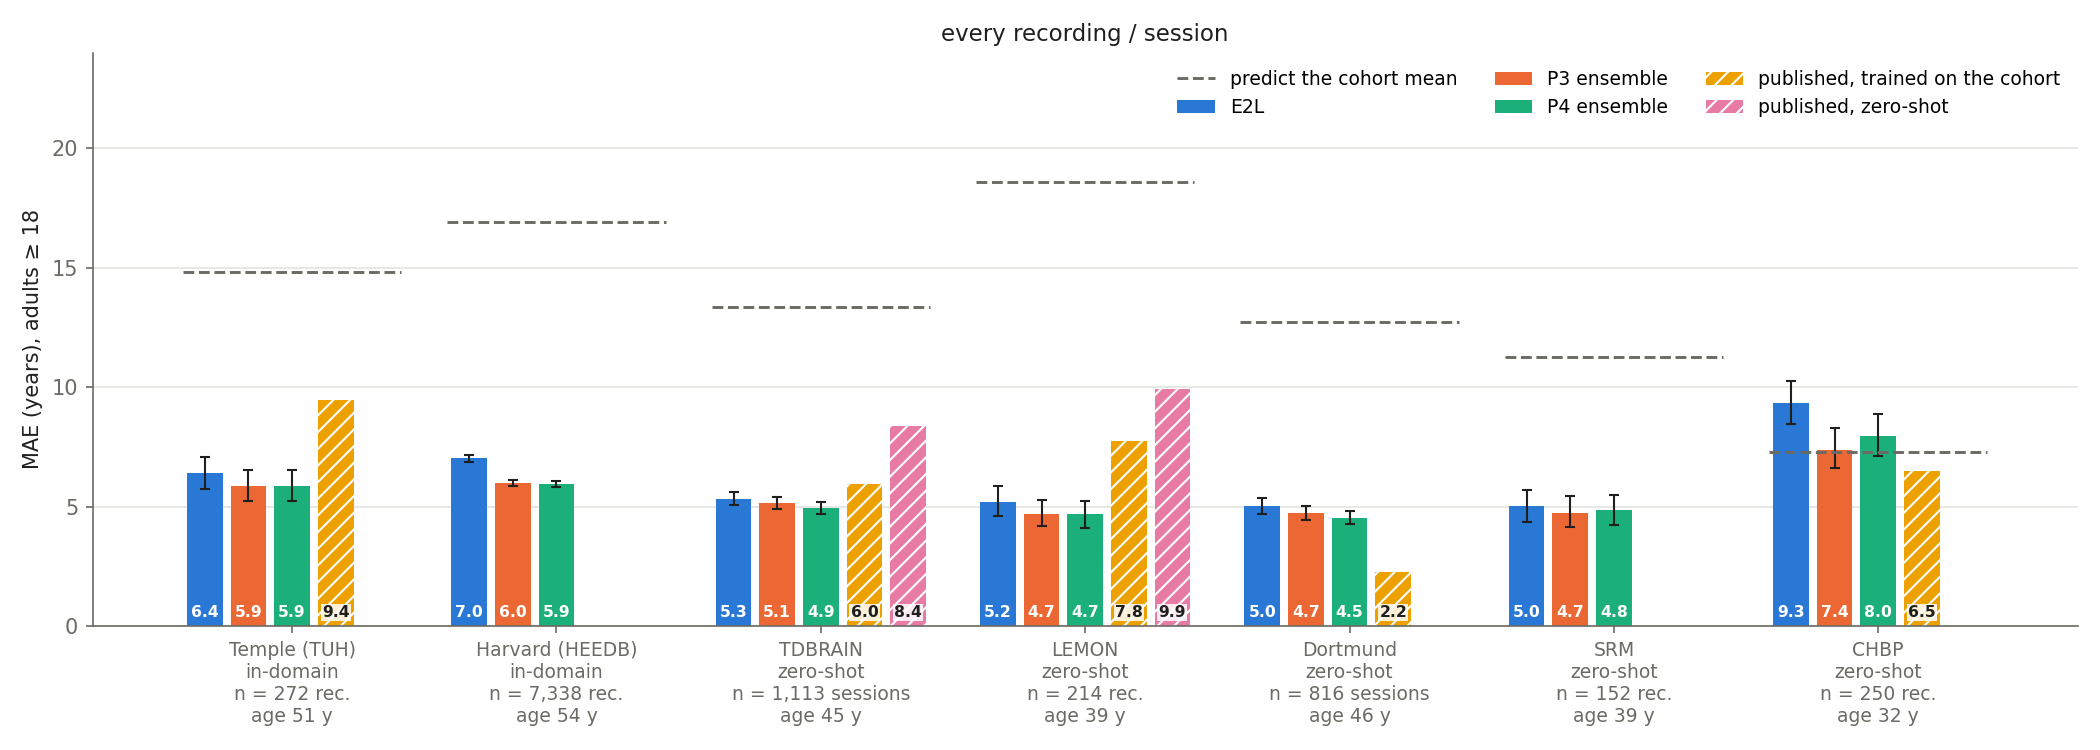
\includegraphics[width=\textwidth,height=0.62\textheight,keepaspectratio]{fig_cohort_mae.png}
\caption{MAE per cohort for E2L and the two ensembles, with 95 \% intervals. Dashed: MAE of predicting the cohort's mean age. Hatched bars: best published MAE, yellow for a model trained on that cohort and pink for a zero-shot model.}
\end{figure}


The subsets of Table 13 are discussed in Section 6.2. The two-step attention models L1 and W4 are close to the ensembles in-domain and best on LEMON (4.51 years for W4) and on Temple's normal recordings (4.41 for L1), but on TDBRAIN and SRM they are no better than the window model and on CHBP only 0.2 to 0.4 years better, while the ensembles stay ahead there: training in one run with five fold models is what makes the attention models robust outside the training data. The ensembles improve on the window model on every cohort, by about 1 year on Harvard and 0.2 to 2.0 years on the external cohorts. P4 is the better recipe where the recording resembles the training data (Harvard, TDBRAIN, LEMON, Dortmund) and P3 under shift (CHBP), which fits P3's smaller gap between training and validation error (2.33 against 2.96 years). On CHBP every model is at or above the MAE of predicting the cohort's mean age ($R^2 \le 0$). A healthy TDBRAIN subgroup of the same age range (18--68 years) is predicted with an MAE of 5.18 years by E2L, so CHBP's error comes from the recording chain, not the population; Section 6.5 measures where the signals differ and what corrects it.

Dortmund and SRM, two research cohorts of healthy volunteers with exact ages, land at the level of TDBRAIN and LEMON. Dortmund is the strongest test of the five: 608 people spread evenly over 20 to 70 years, recorded on a research amplifier. It is predicted as well as healthy Temple recordings of the same ages (P4 ensemble 4.53 against 4.54 years) and better than healthy Harvard ones (5.54), with recordings of the training domain weighted to Dortmund's age distribution (\texttt{docs/dortmund\_onboarding.md} Table 13.4). On SRM, the smallest cohort, the three models are within their intervals of each other. The only published age result on Dortmund (2.24 years) is a conference abstract that trains and tests inside the cohort, without saying whether a person's runs stay in one fold; it is not comparable with a zero-shot score.

\begin{figure}[t]
\centering
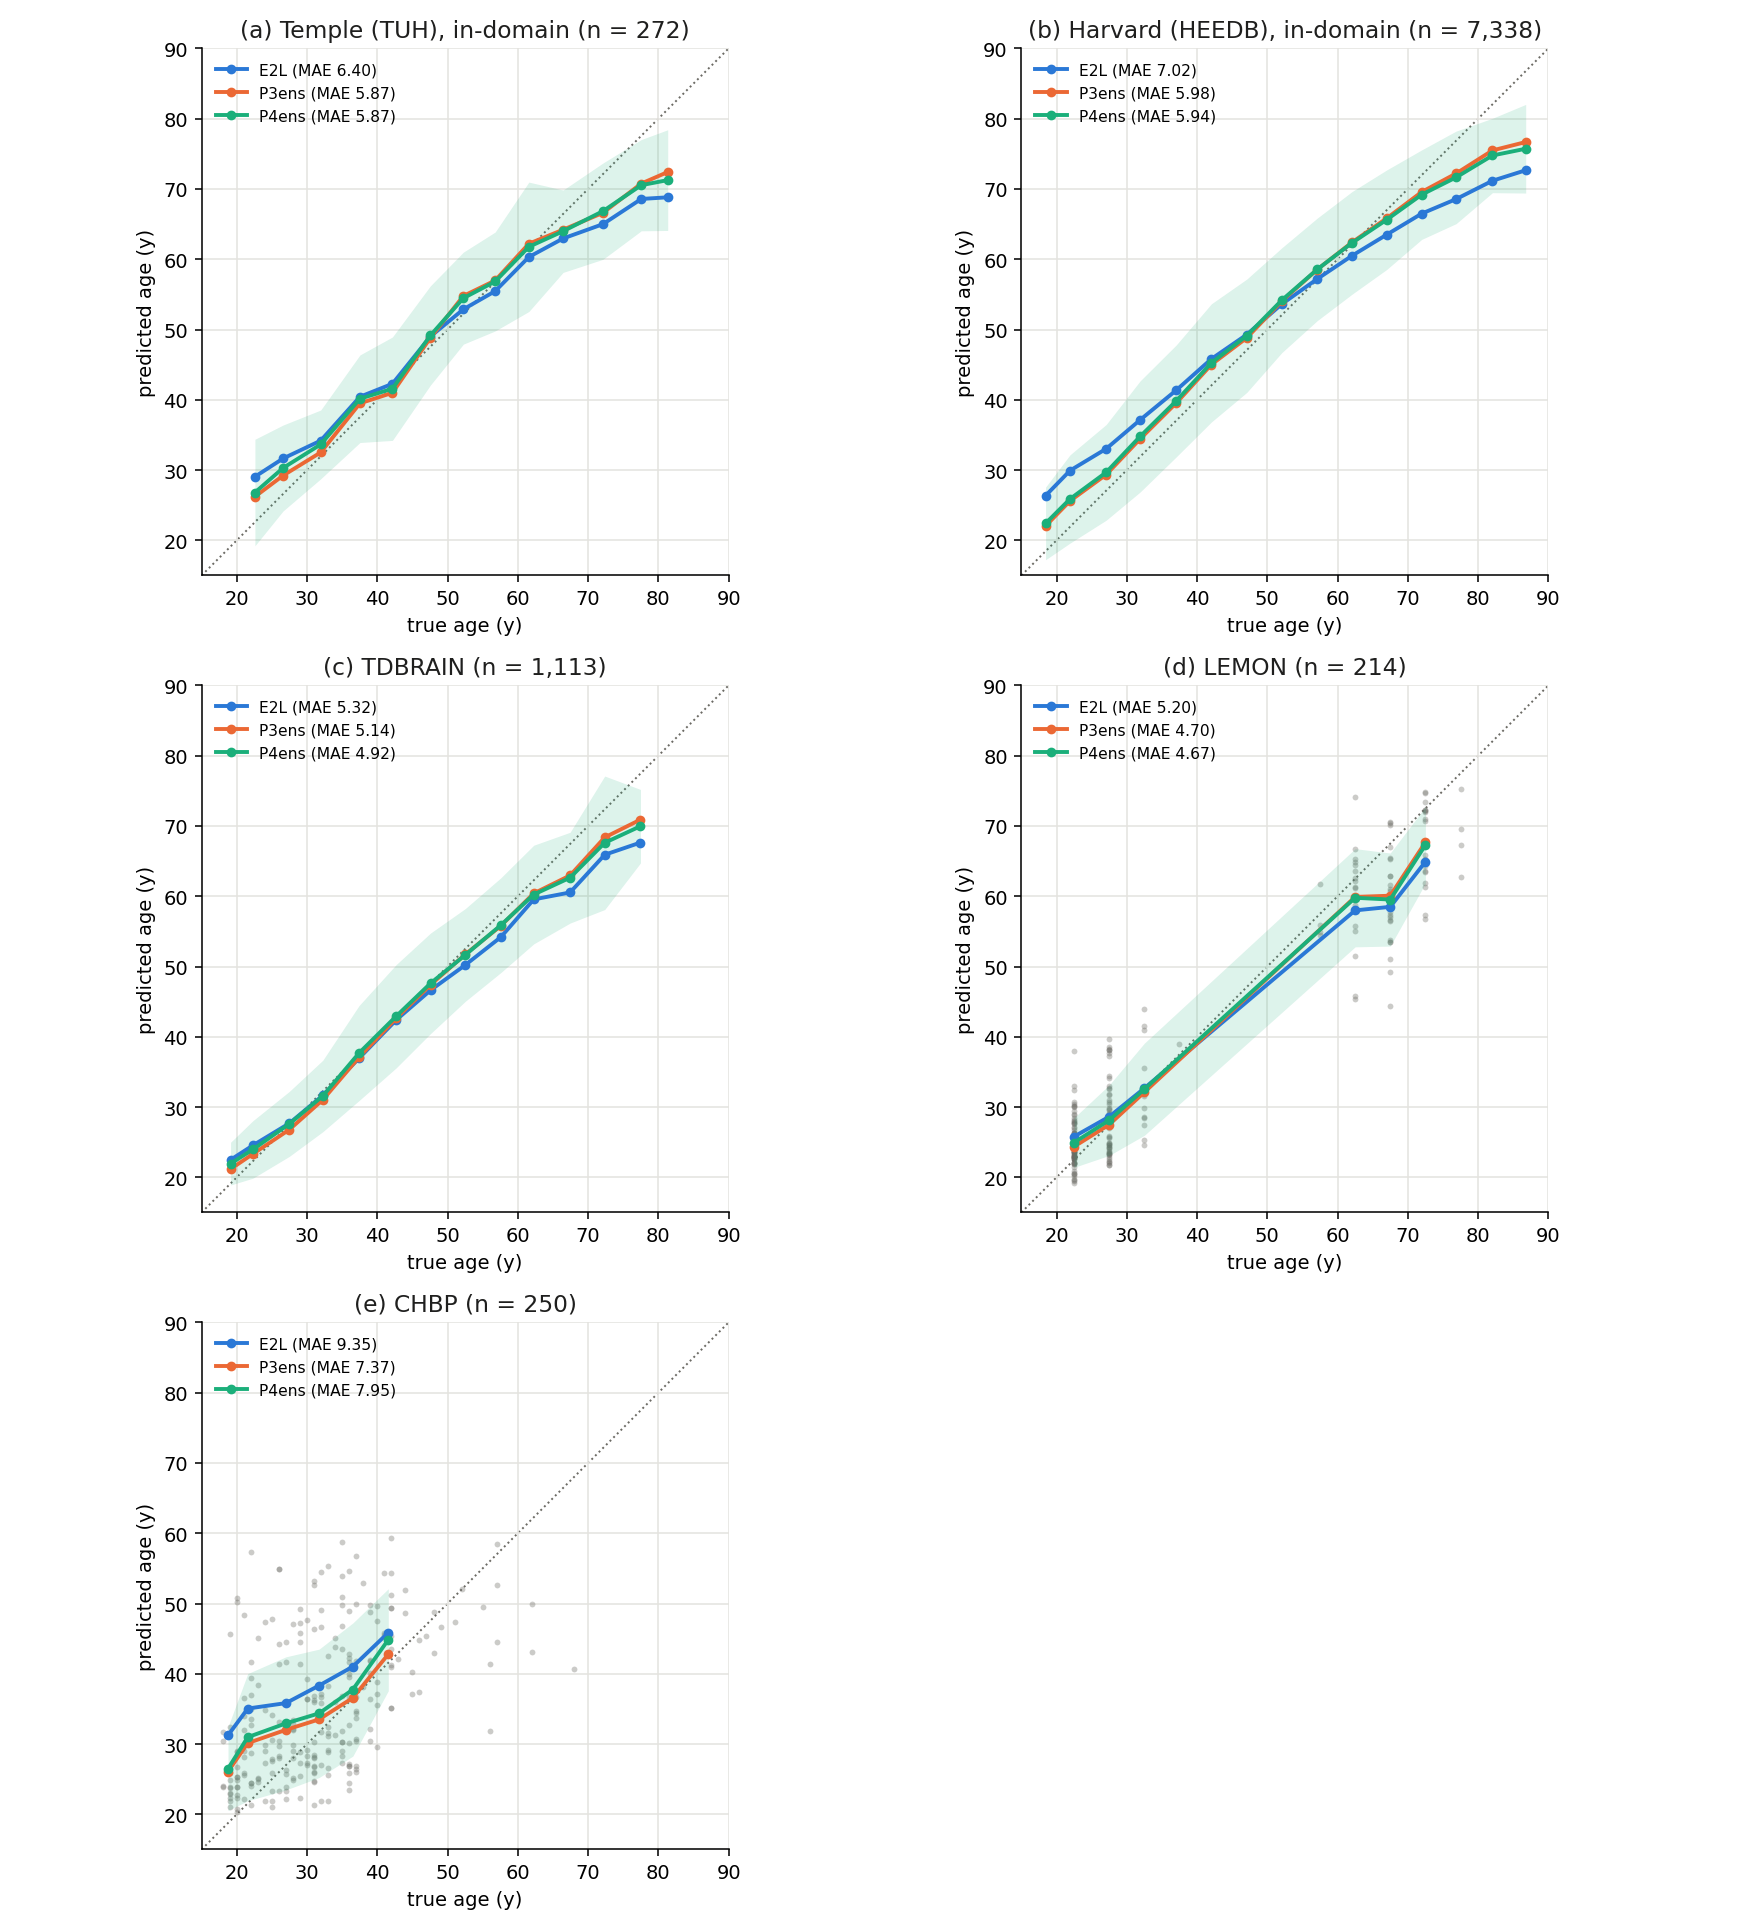
\includegraphics[width=\textwidth,height=0.62\textheight,keepaspectratio]{pred_vs_age_models.png}
\caption{Predicted against true age per cohort: mean prediction per 5-year age bin (bins with at least 10 recordings) for the three models. Band: $\pm$ 1 standard deviation of the P4 ensemble. Dotted: identity. Points are shown for the open cohorts only.}
\end{figure}


\subsection{Report status and pathology groups}

\begin{table}[t]
\centering
\small
\caption{P4 ensemble, MAE in years. Temple and Harvard: EEG report normal or abnormal. TDBRAIN: healthy controls or any indication.}
\begin{tabular}{lll}
\toprule
\textbf{cohort} & \textbf{healthy / normal report} & \textbf{pathological / abnormal report} \\
\midrule
Temple & 4.52 (n = 149, mean age 44.6) & 7.50 (n = 123, mean age 58.0) \\
Harvard & 5.69 (n = 1,518, mean age 48.8) & 6.49 (n = 2,253, mean age 58.8) \\
TDBRAIN & 4.96 (n = 179, mean age 40.3) & 4.92 (n = 934, mean age 46.2) \\
Dortmund & 4.53 (n = 816 sessions, mean age 46.1) & no patients \\
SRM & 4.84 (n = 152, mean age 38.8) & no patients \\
\bottomrule
\end{tabular}
\end{table}


An abnormal EEG report costs accuracy (and those patients are about 10 years older), while a psychiatric indication does not. In TDBRAIN the brain-age gap of major depression (n = 351), ADHD (116), OCD (54) and subjective memory complaints (89) does not differ from that of the healthy controls (179) after adjusting for age, age squared and sex: every adjusted difference is below 1 year, $\lvert t \rvert < 1.1$, with all three models. With these group sizes a difference of about 1.7 years would have been detected for depression (80 \% power).

For the diagnosis groups of the two hospital cohorts we use Eq. (22). The reference is a normal EEG report and a health record with none of the groups. Temple's groups come from the corpus's clinical sheet and Harvard's from the ICD-10 codes of the patient's record; a patient can be in several. The Temple test split is too small for this (272 recordings), so the table uses out-of-fold predictions: each P3 fold model on its own validation fold, which it did not train on (4 of the 5 folds; 24,844 Temple and 51,527 Harvard recordings of adults; one model per recording, no ensemble).

\begin{table}[t]
\centering
\small
\caption{Brain age per diagnosis group, out-of-fold predictions of the P3 fold models. MAE in years; adjusted gap $\beta$ of Eq. (22) in years with a 95 \% interval, for all recordings of the group and for those with a normal and with an abnormal EEG report. Groups overlap. "s." = fewer than 30 recordings, suppressed.}
\resizebox{\textwidth}{!}{%
\begin{tabular}{lllllll}
\toprule
\textbf{cohort, group} & \textbf{recordings} & \textbf{mean age} & \textbf{MAE} & \textbf{adjusted gap} & \textbf{gap, normal report} & \textbf{gap, abnormal report} \\
\midrule
Harvard, reference & 2,248 & 45.0 & 5.44 &  &  &  \\
Harvard, stroke & 5,238 & 65.1 & 6.82 & +2.5 [2.0, 3.0] & +0.7 [0.0, 1.4] & +3.1 [2.5, 3.7] \\
Harvard, dementia & 3,568 & 72.1 & 6.86 & +2.1 [1.5, 2.7] & $-$0.1 [$-$0.9, 0.7] & +2.6 [1.9, 3.3] \\
Harvard, multiple sclerosis & 677 & 51.4 & 6.80 & +2.0 [1.2, 2.8] & +0.6 [$-$0.7, 1.8] & +3.5 [2.2, 4.8] \\
Harvard, movement disorders & 6,801 & 58.7 & 6.58 & +1.8 [1.4, 2.2] & +0.5 [0.0, 1.0] & +2.7 [2.2, 3.2] \\
Harvard, CNS tumours & 2,954 & 57.3 & 6.67 & +1.4 [0.9, 1.8] & +0.2 [$-$0.5, 1.0] & +1.5 [0.9, 2.1] \\
Harvard, depression & 9,318 & 55.4 & 6.28 & +1.3 [1.0, 1.7] & +0.5 [0.0, 0.9] & +2.2 [1.8, 2.7] \\
Harvard, electrographic seizures & 3,749 & 54.1 & 6.56 & +1.1 [0.6, 1.5] & +0.2 [$-$0.4, 0.7] & +1.6 [1.1, 2.1] \\
Harvard, sleep disorders & 10,395 & 57.5 & 6.28 & +1.1 [0.7, 1.4] & $-$0.2 [$-$0.6, 0.3] & +2.3 [1.8, 2.8] \\
Harvard, headache and migraine & 12,932 & 53.9 & 6.10 & +0.8 [0.5, 1.2] & $-$0.2 [$-$0.6, 0.2] & +1.9 [1.4, 2.3] \\
Harvard, epilepsy & 16,450 & 50.0 & 5.98 & +0.6 [0.3, 1.0] & +0.1 [$-$0.3, 0.5] & +1.4 [1.0, 1.7] \\
Temple, reference & 8,335 & 48.5 & 6.77 &  &  &  \\
Temple, substance use & 933 & 46.7 & 8.05 & +3.3 [2.2, 4.3] & +1.5 [0.2, 2.7] & +3.9 [2.6, 5.3] \\
Temple, traumatic brain injury & 273 & 45.2 & 8.60 & +2.6 [0.0, 5.1] & +3.8 [$-$0.2, 7.9] & +2.0 [$-$1.2, 5.2] \\
Temple, stroke & 856 & 62.5 & 8.66 & +1.9 [0.6, 3.2] & $-$0.5 [$-$3.5, 2.4] & +2.3 [1.0, 3.7] \\
Temple, bipolar disorder & 261 & 44.9 & 6.43 & +1.7 [0.3, 3.1] & +1.0 [$-$1.1, 3.0] & +2.1 [0.3, 4.0] \\
Temple, clinical seizures & 1,762 & 47.6 & 6.68 & +0.2 [$-$0.6, 1.0] & $-$0.7 [$-$1.6, 0.3] & +0.8 [$-$0.2, 1.9] \\
Temple, epilepsy & 631 & 49.3 & 7.18 & +0.0 [$-$1.3, 1.3] & $-$0.2 [$-$2.1, 1.8] & +0.2 [$-$1.5, 1.9] \\
\bottomrule
\end{tabular}
}
\end{table}


\begin{figure}[t]
\centering
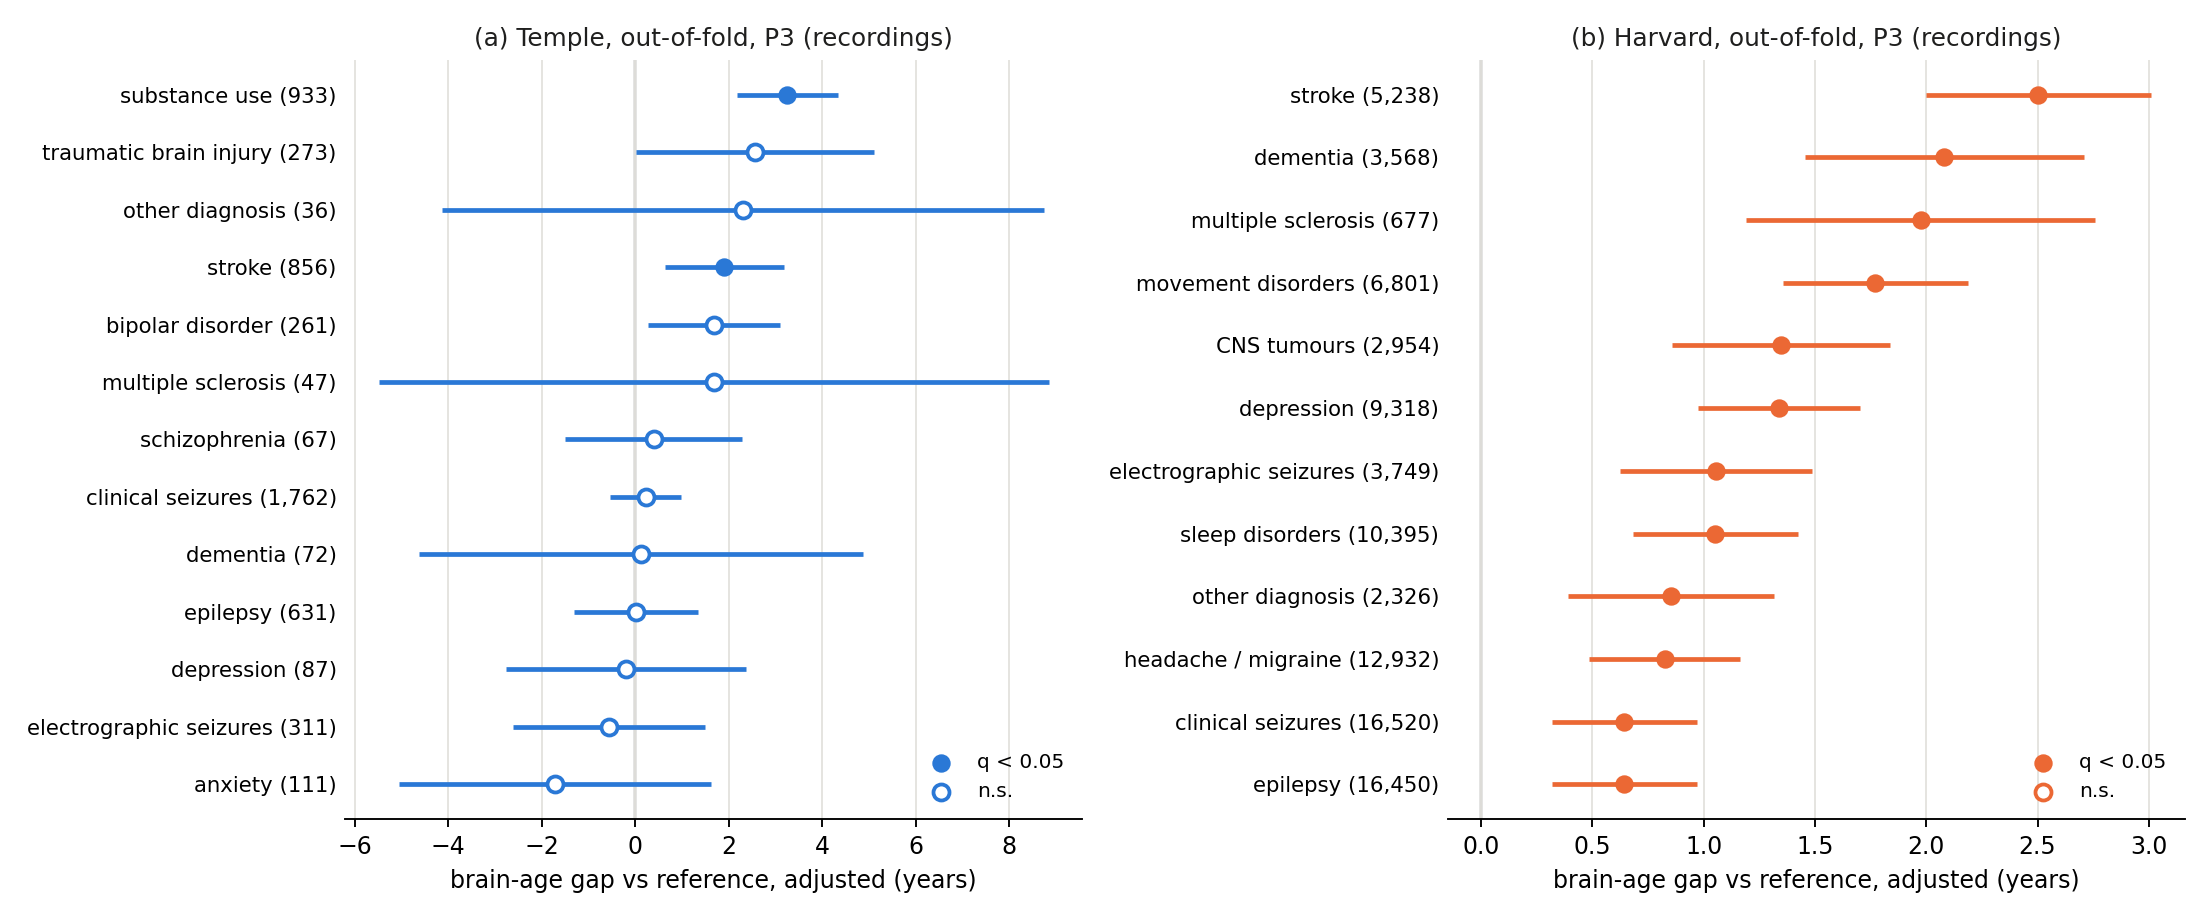
\includegraphics[width=\textwidth,height=0.62\textheight,keepaspectratio]{../figures/tdbrain/pathology_gap.png}
\caption{Adjusted brain-age gap of each diagnosis group against the reference, Eq. (22), with 95 \% intervals; out-of-fold predictions of the P3 fold models. Filled markers: false discovery rate below 0.05. Recordings per group in brackets.}
\end{figure}


Three results stand out (Table 15, Figure 15).

\begin{itemize}
\item \textbf{Accuracy is close to uniform across diagnoses.} The MAE per Harvard group is 6.0 to 6.9 years against 5.4 for the reference, and most of that is age: at the same age and sex the extra absolute error is 0.3 to 1.2 years. An abnormal report costs about 1 year of absolute error in both cohorts.
\item \textbf{Every Harvard diagnosis group looks older than the reference,} from 0.6 years for epilepsy to 2.5 years for stroke; all are significant after the false-discovery adjustment. The held-out test split with the P4 ensemble gives the same order (stroke +2.5, dementia +3.0, epilepsy +0.7 years). In Temple, substance use (+3.3) and stroke (+1.9) are significant.
\item \textbf{The gap goes with the abnormal EEG, not with the diagnosis.} A patient with a diagnosis and a normal EEG report is within about 0.7 years of the reference in every Harvard group of Table 15; with an abnormal report the same group looks 1.4 to 3.5 years older. Among Harvard recordings with a normal report, any diagnosis against none gives $-$0.05 years [$-$0.38, 0.29]. An abnormal against a normal report gives +1.8 years [1.4, 2.3] without any diagnosis and +1.9 years [1.7, 2.1] with one; in Temple +2.1 and +2.6 years.
\end{itemize}

Two cautions. The estimate averages over the ages of a group: among patients of 60 and over, the Harvard gaps of stroke, dementia and movement disorders are about half as large (+1.2, +1.2 and +0.8 years, all above 0), because the compression of the predictions limits how much older an old patient can look. And Harvard's diagnoses are codes anywhere in the patient's record, not the reason for the EEG.

Published work points the same way with other signals. In sleep EEG, patients with neurological or psychiatric disease had a mean excess brain age of 4 years~\citep{sun2019sleep}, and structural MRI shows apparent brain ageing in several brain disorders~\citep{kaufmann2019common}. For routine EEG, Gemein et al.~\citep{gemein2024revisited} report a lower gap in pathological than in non-pathological TUAB recordings (the age is under-estimated by 5 against 1 years) with a model trained on normal recordings only. Our raw difference between abnormal and normal reports is between $-$0.9 and +0.6 years depending on the model and cohort, and it becomes about +2 years once age is adjusted for, so the sign of this comparison depends on how the age bias is treated.

\subsection{Selective prediction}

\begin{table}[t]
\centering
\small
\caption{P4 ensemble, MAE in years of the 80 \% most confident recordings of each cohort, by rejection score, and the MAE an oracle would reach by rejecting the largest true errors.}
\resizebox{\textwidth}{!}{%
\begin{tabular}{llllllll}
\toprule
\textbf{score} & \textbf{Temple} & \textbf{Harvard} & \textbf{TDBRAIN} & \textbf{LEMON} & \textbf{Dortmund} & \textbf{SRM} & \textbf{CHBP} \\
\midrule
no rejection & 5.87 & 5.94 & 4.92 & 4.67 & 4.53 & 4.84 & 7.95 \\
spread, Eq. (13) & 5.69 & 5.56 & 4.54 & \textbf{3.79} & \textbf{4.24} & 4.60 & 7.84 \\
total, Eq. (14) & \textbf{5.07} & \textbf{5.32} & \textbf{4.53} & 3.80 & 4.32 & 4.60 & \textbf{7.03} \\
learned & 5.11 & 5.34 & 4.57 & 3.81 & 4.32 & \textbf{4.39} & 7.43 \\
oracle & 3.78 & 3.83 & 3.25 & 2.92 & 3.09 & 3.23 & 5.06 \\
\bottomrule
\end{tabular}
}
\end{table}


\begin{figure}[t]
\centering
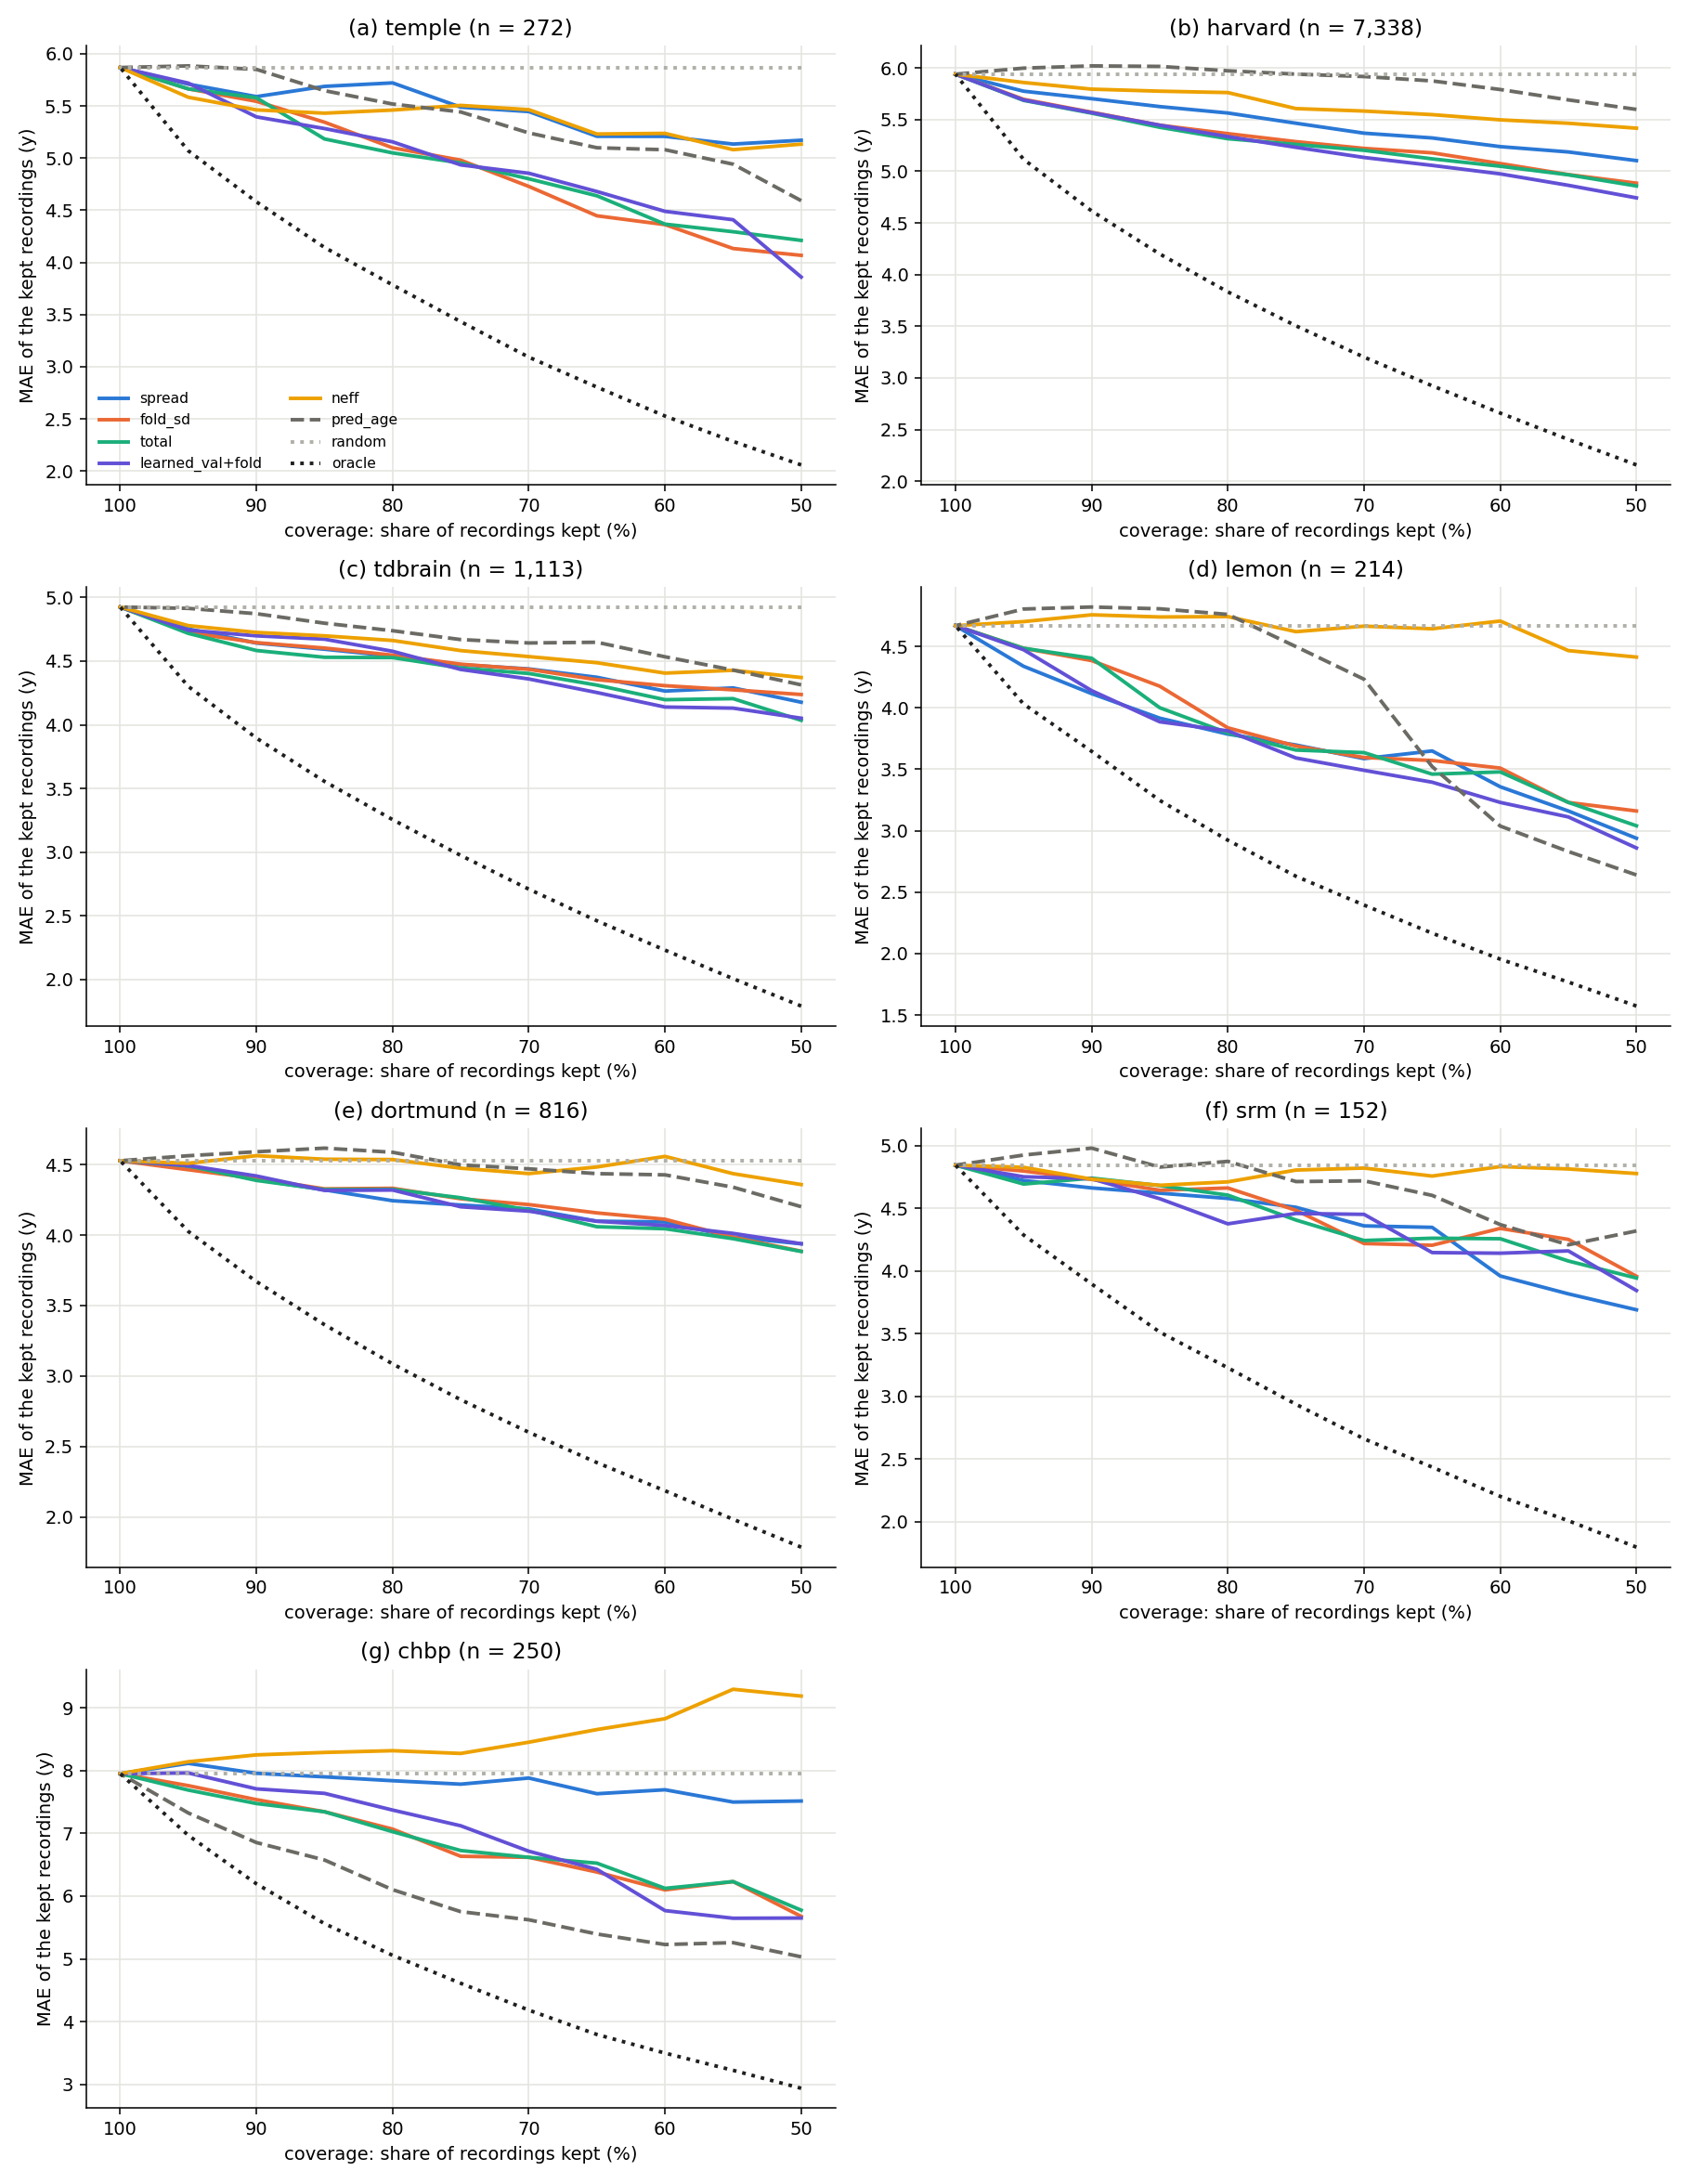
\includegraphics[width=\textwidth,height=0.62\textheight,keepaspectratio]{fig_rejection_curves.png}
\caption{Risk--coverage curves of the P4 ensemble: MAE of the kept recordings against the share kept, per cohort, for several scores. \texttt{neff} is an attention-only score (the effective share of windows attended), \texttt{pred\_age} rejects the oldest predictions, \texttt{random} is no information and \texttt{oracle} rejects by the true error.}
\end{figure}


Rejection by the combined score lowers the MAE on every cohort, by 0.2 to 0.9 years on the external ones. It is never significantly worse than the spread and is significantly better on Temple, Harvard and CHBP (paired bootstrap), because the disagreement of the fold models sees errors that are shared by all windows of a recording. Scores built from the attention weights alone are weak and change sign on CHBP. Two cautions apply. The scores were compared on the test cohorts, so the choice among them is not independent of these data. And part of every score is age: within deciles of the predicted age, the combined score keeps 60 to 80 \% of its gain on Temple, Harvard and TDBRAIN, about half on Dortmund, all of it on SRM, but nothing on LEMON and CHBP. The combined score recovers 15 to 50 \% of what the oracle would (15 \% on Dortmund and SRM, where the errors are small and even). On Dortmund the rejected sessions are the older ones, not the outliers: their mean age is 51 to 55 years against 44 to 45 for the kept ones (\texttt{docs/dortmund\_onboarding.md} Table 13.5).

\textbf{Inside the recording.} Figures 17 and 18 relate the error of single windows to the quantities of Eqs. (20) and (21) for the P4 ensemble.

\begin{figure}[t]
\centering
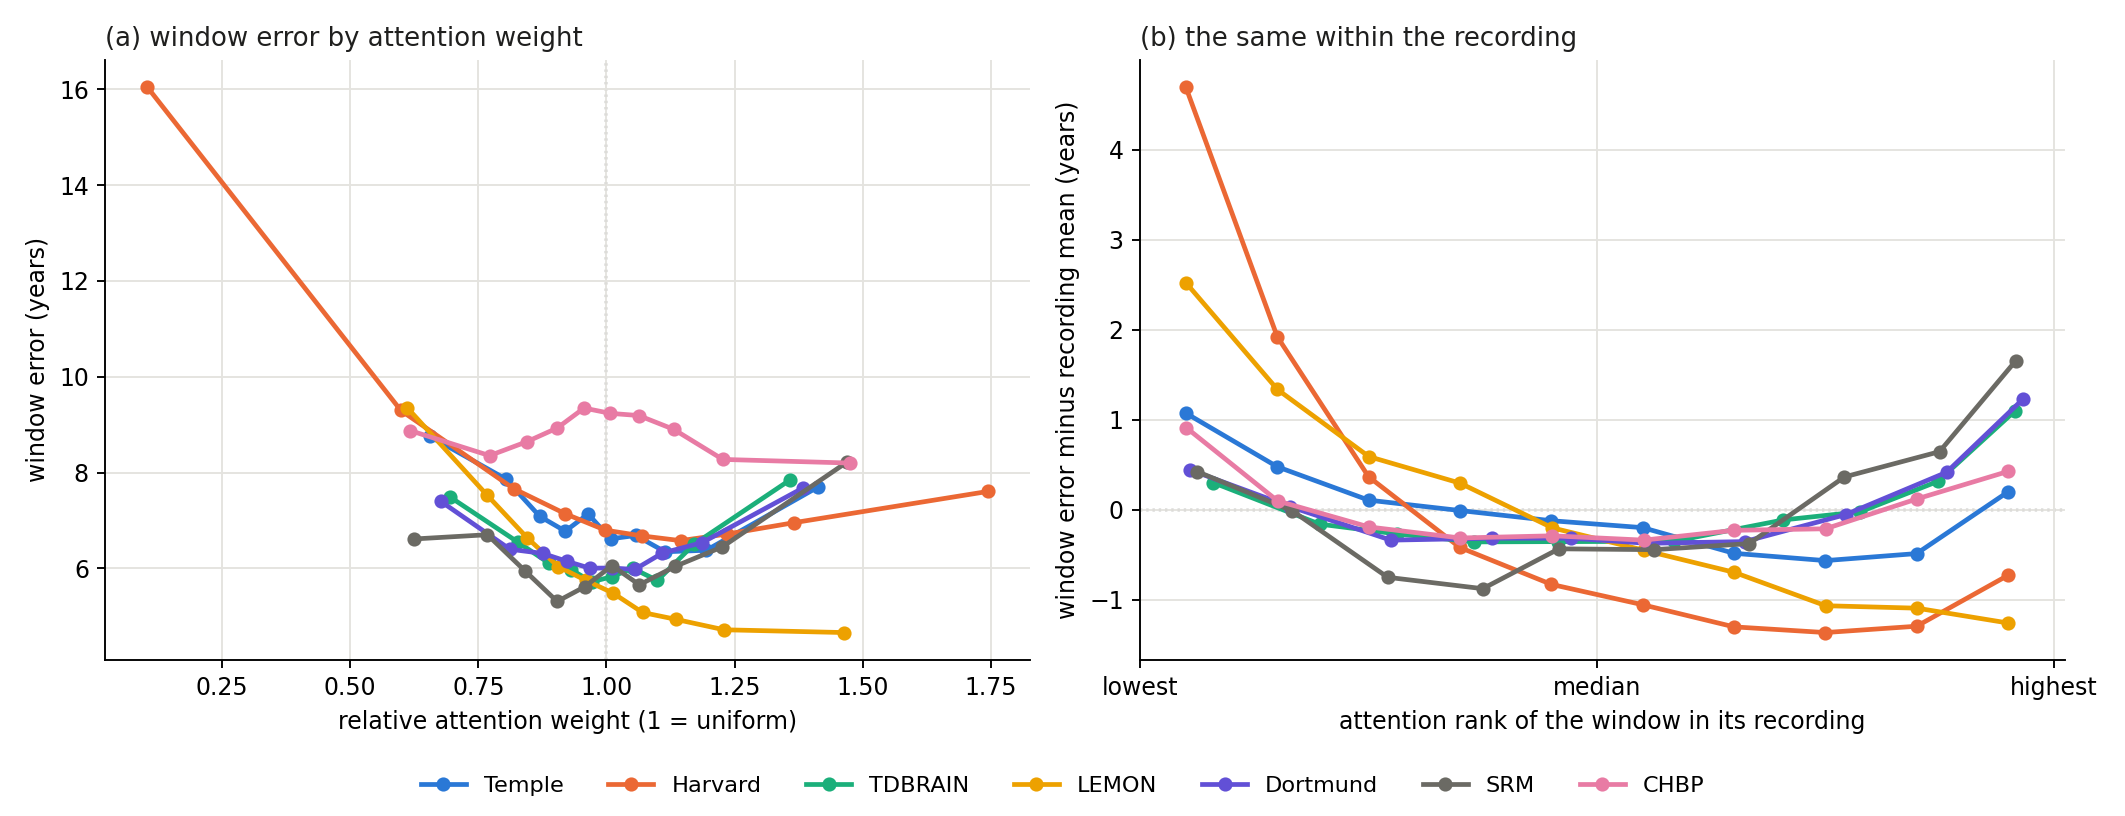
\includegraphics[width=\textwidth,height=0.62\textheight,keepaspectratio]{window_error_vs_attention.png}
\caption{Window error against the attention weight, P4 ensemble. (a) Mean window error per decile of the relative attention weight. (b) The same inside the recording: the window's error minus the mean window error of its recording, per decile of the window's attention rank in the recording. Binned means.}
\end{figure}


\begin{figure}[t]
\centering
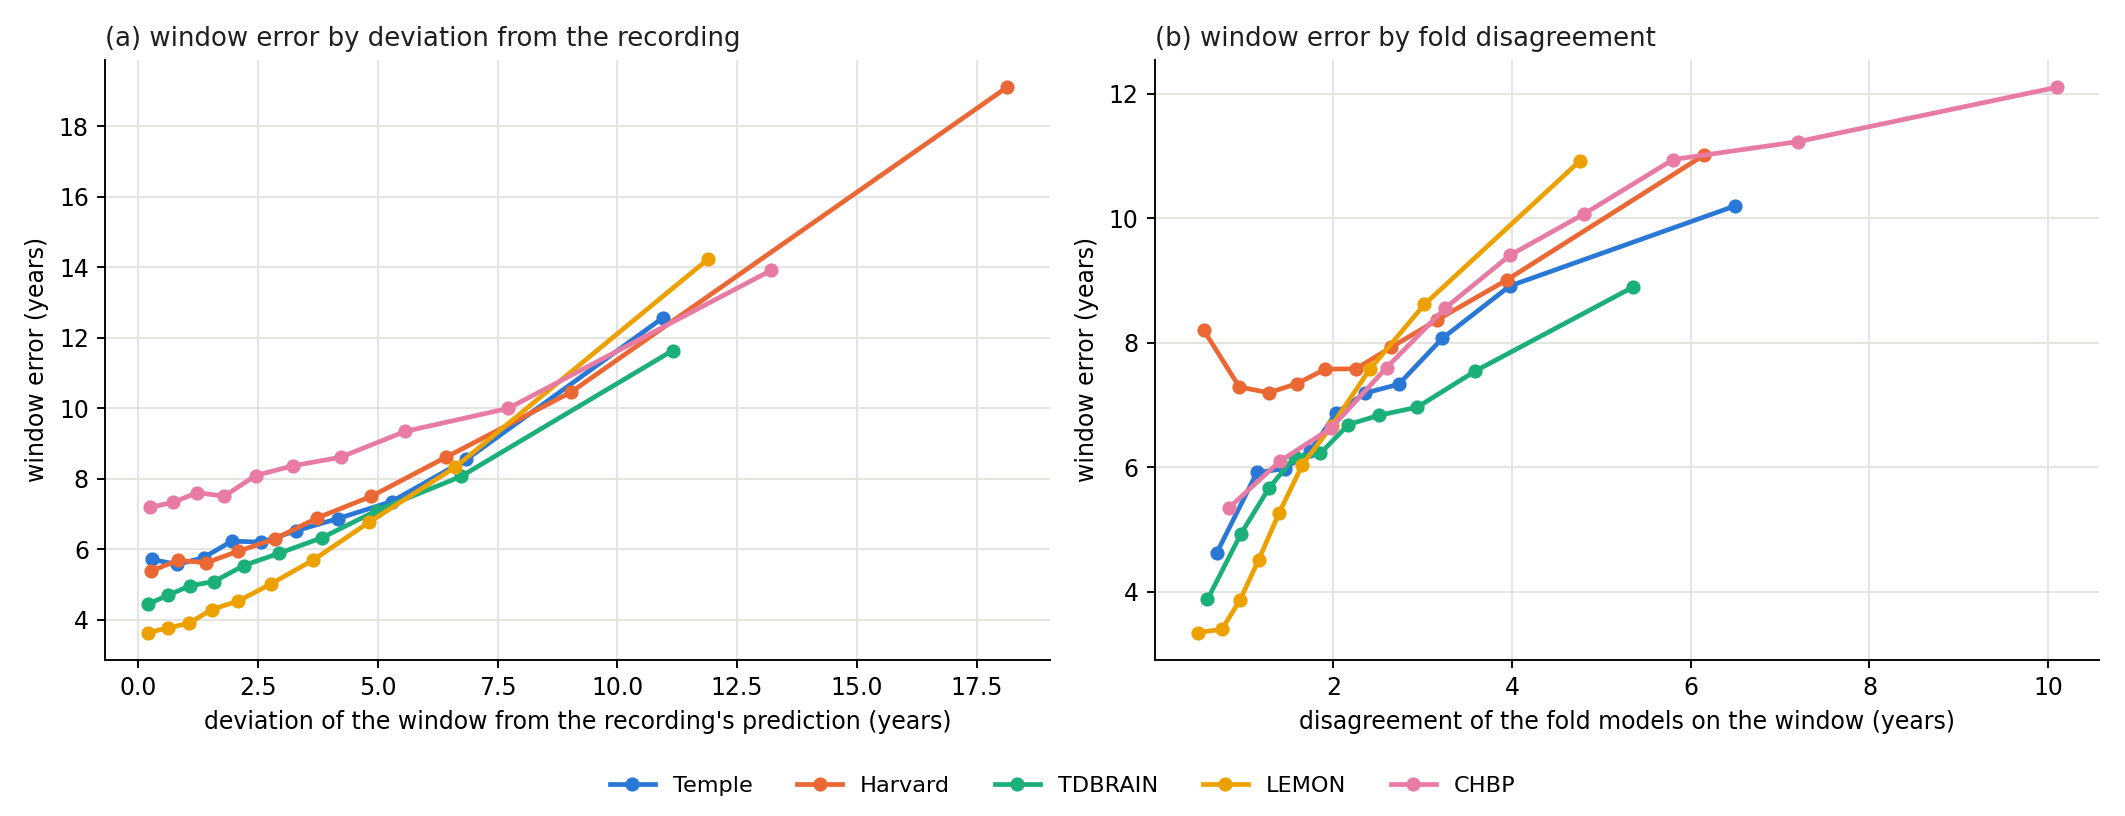
\includegraphics[width=\textwidth,height=0.62\textheight,keepaspectratio]{window_error_vs_spread.png}
\caption{Window error (a) per decile of the window's deviation from the recording's prediction and (b) per decile of the disagreement of the fold models on the window, P4 ensemble. Binned means.}
\end{figure}


\begin{itemize}
\item \textbf{Attention removes bad windows more than it selects good ones.} The windows with the lowest weight are much worse than the rest (Harvard: 16 years at a tenth of the uniform weight against about 7), but above the median weight the error is flat, and in Temple, TDBRAIN and CHBP the highest-weight windows are worse again.
\item \textbf{On the four short research recordings and CHBP the weight carries no information about the window.} Inside a recording its rank correlation with the window error has a median of +0.08 to +0.15 on TDBRAIN, Dortmund, SRM and CHBP, against $-$0.08 to $-$0.27 on Temple, Harvard and LEMON, and attention pooling does not beat the plain mean of the window predictions there (5.36 against 5.32 years per TDBRAIN file, 5.16 against 5.14 per Dortmund run, 4.84 against 4.65 on SRM). Where it works it is worth 0.2 years on Temple, 0.7 on Harvard and 0.4 on LEMON.
\item \textbf{Deviation from the recording's prediction is the strongest window signal.} Inside a recording its rank correlation with the window error is 0.21 to 0.44, and the error grows from 4 to 7 years for the tenth of the windows closest to the recording's prediction to 12 to 19 years for the most deviant tenth. This is what makes the spread usable, and it favours robust pooling over more attention capacity.
\item \textbf{Fold disagreement is a recording-level signal.} Over all windows it follows the error (rank correlation 0.16 to 0.39), but inside a recording it does not (median between $-$0.07 and +0.01 on six of the seven cohorts, 0.14 on LEMON): the fold models disagree on whole recordings, which is the part the combined score adds to the spread.
\end{itemize}

\textbf{Window trimming by attention weight.} Rejection sets whole recordings aside; trimming keeps every recording and drops, inside it, the windows the attention pool trusts least. With $w_{ik} = n\,\alpha_{ik}$ the relative weight of window $i$ for fold model $k$ (Eq. (20) before averaging over the fold models; 1 = uniform), each fold model keeps the windows at or above a threshold $\tau$, at least its most confident window, and re-pools them (the attention rule of \texttt{scripts/confidence\_thresholds.py}, \texttt{docs/external\_eval\_results.md} Section 7, here applied to the cross-validation ensembles):

\begin{equation}
\mathcal{K}_k(\tau) = \{\, i : w_{ik} \ge \tau \,\} \cup \{\arg\max_i w_{ik}\}, \qquad \hat y_{r,k}(\tau) = \frac{\sum_{i \in \mathcal{K}_k(\tau)} \alpha_{ik}\, p_{ik}}{\sum_{i \in \mathcal{K}_k(\tau)} \alpha_{ik}}, \qquad \tau_q = Q_q\big( w \text{ on validation} \big) \tag{23}
\end{equation}

which is exact for the softmax pool followed by the linear head, so no model is re-run. The three thresholds are fixed once, without labels, as the 10th, 25th and 50th percentiles of $w$ over the validation windows of the fold models (each on its own validation fold at its best epoch; adults, first 5 minutes): \textbf{low} $\tau = 0.53$, \textbf{medium} $\tau = 0.80$, \textbf{high} $\tau = 1.00$ (every window weighted below uniform is dropped). A fourth threshold is the one \texttt{confidence\_thresholds.py} would choose: the value of a grid of $\tau$ (0 to 2 in steps of 0.05, 0 = no trimming) with the lowest validation MAE, \textbf{selected} $\tau = 0.45$ (validation labels, but no test data; the earlier window-trimming analysis chose 0.35 to 0.55 for six older attention models, \texttt{docs/external\_eval\_results.md} Table 7.1). No threshold is computed on a test cohort. The ensemble is the mean of the trimmed fold models. Validation is scored per fold model (each recording by the one model it was held out from), the test cohorts by the five-model ensemble, both on the protocol of Table 21. Table 17 gives the MAE, Table 18 how much is trimmed, and Figure 19 shows the thresholds, one recording and the effect per cohort (\texttt{scripts/window\_trimming.py}).

\begin{table}[t]
\centering
\small
\caption{Window trimming by attention weight, P4, thresholds fixed on validation: MAE in years and, in brackets, the change against no trimming; \texttt{*}: the 95 \% paired bootstrap interval of the change (resampling people) excludes 0. Validation: single fold models on their own validation folds (Temple and Harvard, adults, first 5 minutes); test: the ensemble. \texttt{plain mean}: the mean of all window predictions, without attention.}
\resizebox{\textwidth}{!}{%
\begin{tabular}{llllllll}
\toprule
\textbf{cohort} & \textbf{units} & \textbf{no trimming} & \textbf{low} & \textbf{medium} & \textbf{high} & \textbf{selected on validation} & \textbf{plain mean} \\
\midrule
Temple validation & 18,643 & 7.54 [7.35, 7.72] & 7.55 (+0.01*) & 7.63 (+0.10*) & 7.87 (+0.34*) & 7.54 (0.00*) & 7.55 (+0.01) \\
Harvard validation & 38,468 & 6.17 [6.11, 6.23] & 6.15 ($-$0.01*) & 6.18 (+0.01*) & 6.31 (+0.14*) & 6.15 ($-$0.01*) & 6.80 (+0.63*) \\
Temple test & 272 & 5.87 [5.25, 6.54] & 5.86 ($-$0.01) & 5.79 ($-$0.08) & 5.84 ($-$0.03) & 5.86 (0.00) & 6.04 (+0.17*) \\
Harvard test & 7,338 & 5.94 [5.82, 6.07] & 5.92 ($-$0.02*) & 5.91 ($-$0.03*) & 5.96 (+0.02) & 5.92 ($-$0.02*) & 6.60 (+0.66*) \\
TDBRAIN & 1,113 & 4.92 [4.68, 5.19] & 4.92 (0.00) & 4.99 (+0.06*) & 5.30 (+0.37*) & 4.92 (0.00) & 4.92 ($-$0.01) \\
LEMON & 214 & 4.67 [4.11, 5.24] & 4.63 ($-$0.04*) & 4.44 ($-$0.22*) & 4.28 ($-$0.39*) & 4.66 ($-$0.01) & 5.06 (+0.39*) \\
Dortmund & 816 & 4.53 [4.25, 4.82] & 4.53 (0.00) & 4.58 (+0.05) & 4.78 (+0.25*) & 4.53 (0.00) & 4.55 (+0.02) \\
SRM & 152 & 4.84 [4.23, 5.50] & 4.89 (+0.05*) & 5.22 (+0.37*) & 5.72 (+0.87*) & 4.87 (+0.03*) & 4.65 ($-$0.19*) \\
CHBP & 250 & 7.95 [7.11, 8.87] & 7.99 (+0.04) & 8.10 (+0.15) & 8.26 (+0.31*) & 7.97 (+0.02) & 7.92 ($-$0.03) \\
\bottomrule
\end{tabular}
}
\end{table}


\begin{table}[t]
\centering
\small
\caption{Share of the windows trimmed at each threshold and, in brackets, the share of units whose prediction changes by more than 0.05 years.}
\resizebox{\textwidth}{!}{%
\begin{tabular}{lllll}
\toprule
\textbf{cohort} & \textbf{low} & \textbf{medium} & \textbf{high} & \textbf{selected on validation} \\
\midrule
Temple validation & 3 \% (29 \%) & 22 \% (89 \%) & 55 \% (98 \%) & 2 \% (17 \%) \\
Harvard validation & 14 \% (70 \%) & 27 \% (93 \%) & 47 \% (98 \%) & 13 \% (63 \%) \\
Temple test & 2 \% (33 \%) & 20 \% (94 \%) & 55 \% (98 \%) & 1 \% (17 \%) \\
Harvard test & 14 \% (74 \%) & 27 \% (95 \%) & 48 \% (98 \%) & 12 \% (67 \%) \\
TDBRAIN & 1 \% (26 \%) & 17 \% (94 \%) & 53 \% (99 \%) & 1 \% (14 \%) \\
LEMON & 3 \% (47 \%) & 23 \% (98 \%) & 53 \% (99 \%) & 1 \% (23 \%) \\
Dortmund & 1 \% (31 \%) & 18 \% (94 \%) & 54 \% (99 \%) & 1 \% (12 \%) \\
SRM & 3 \% (45 \%) & 23 \% (97 \%) & 54 \% (99 \%) & 1 \% (24 \%) \\
CHBP & 5 \% (65 \%) & 28 \% (98 \%) & 55 \% (99 \%) & 3 \% (45 \%) \\
\bottomrule
\end{tabular}
}
\end{table}


\begin{figure}[t]
\centering
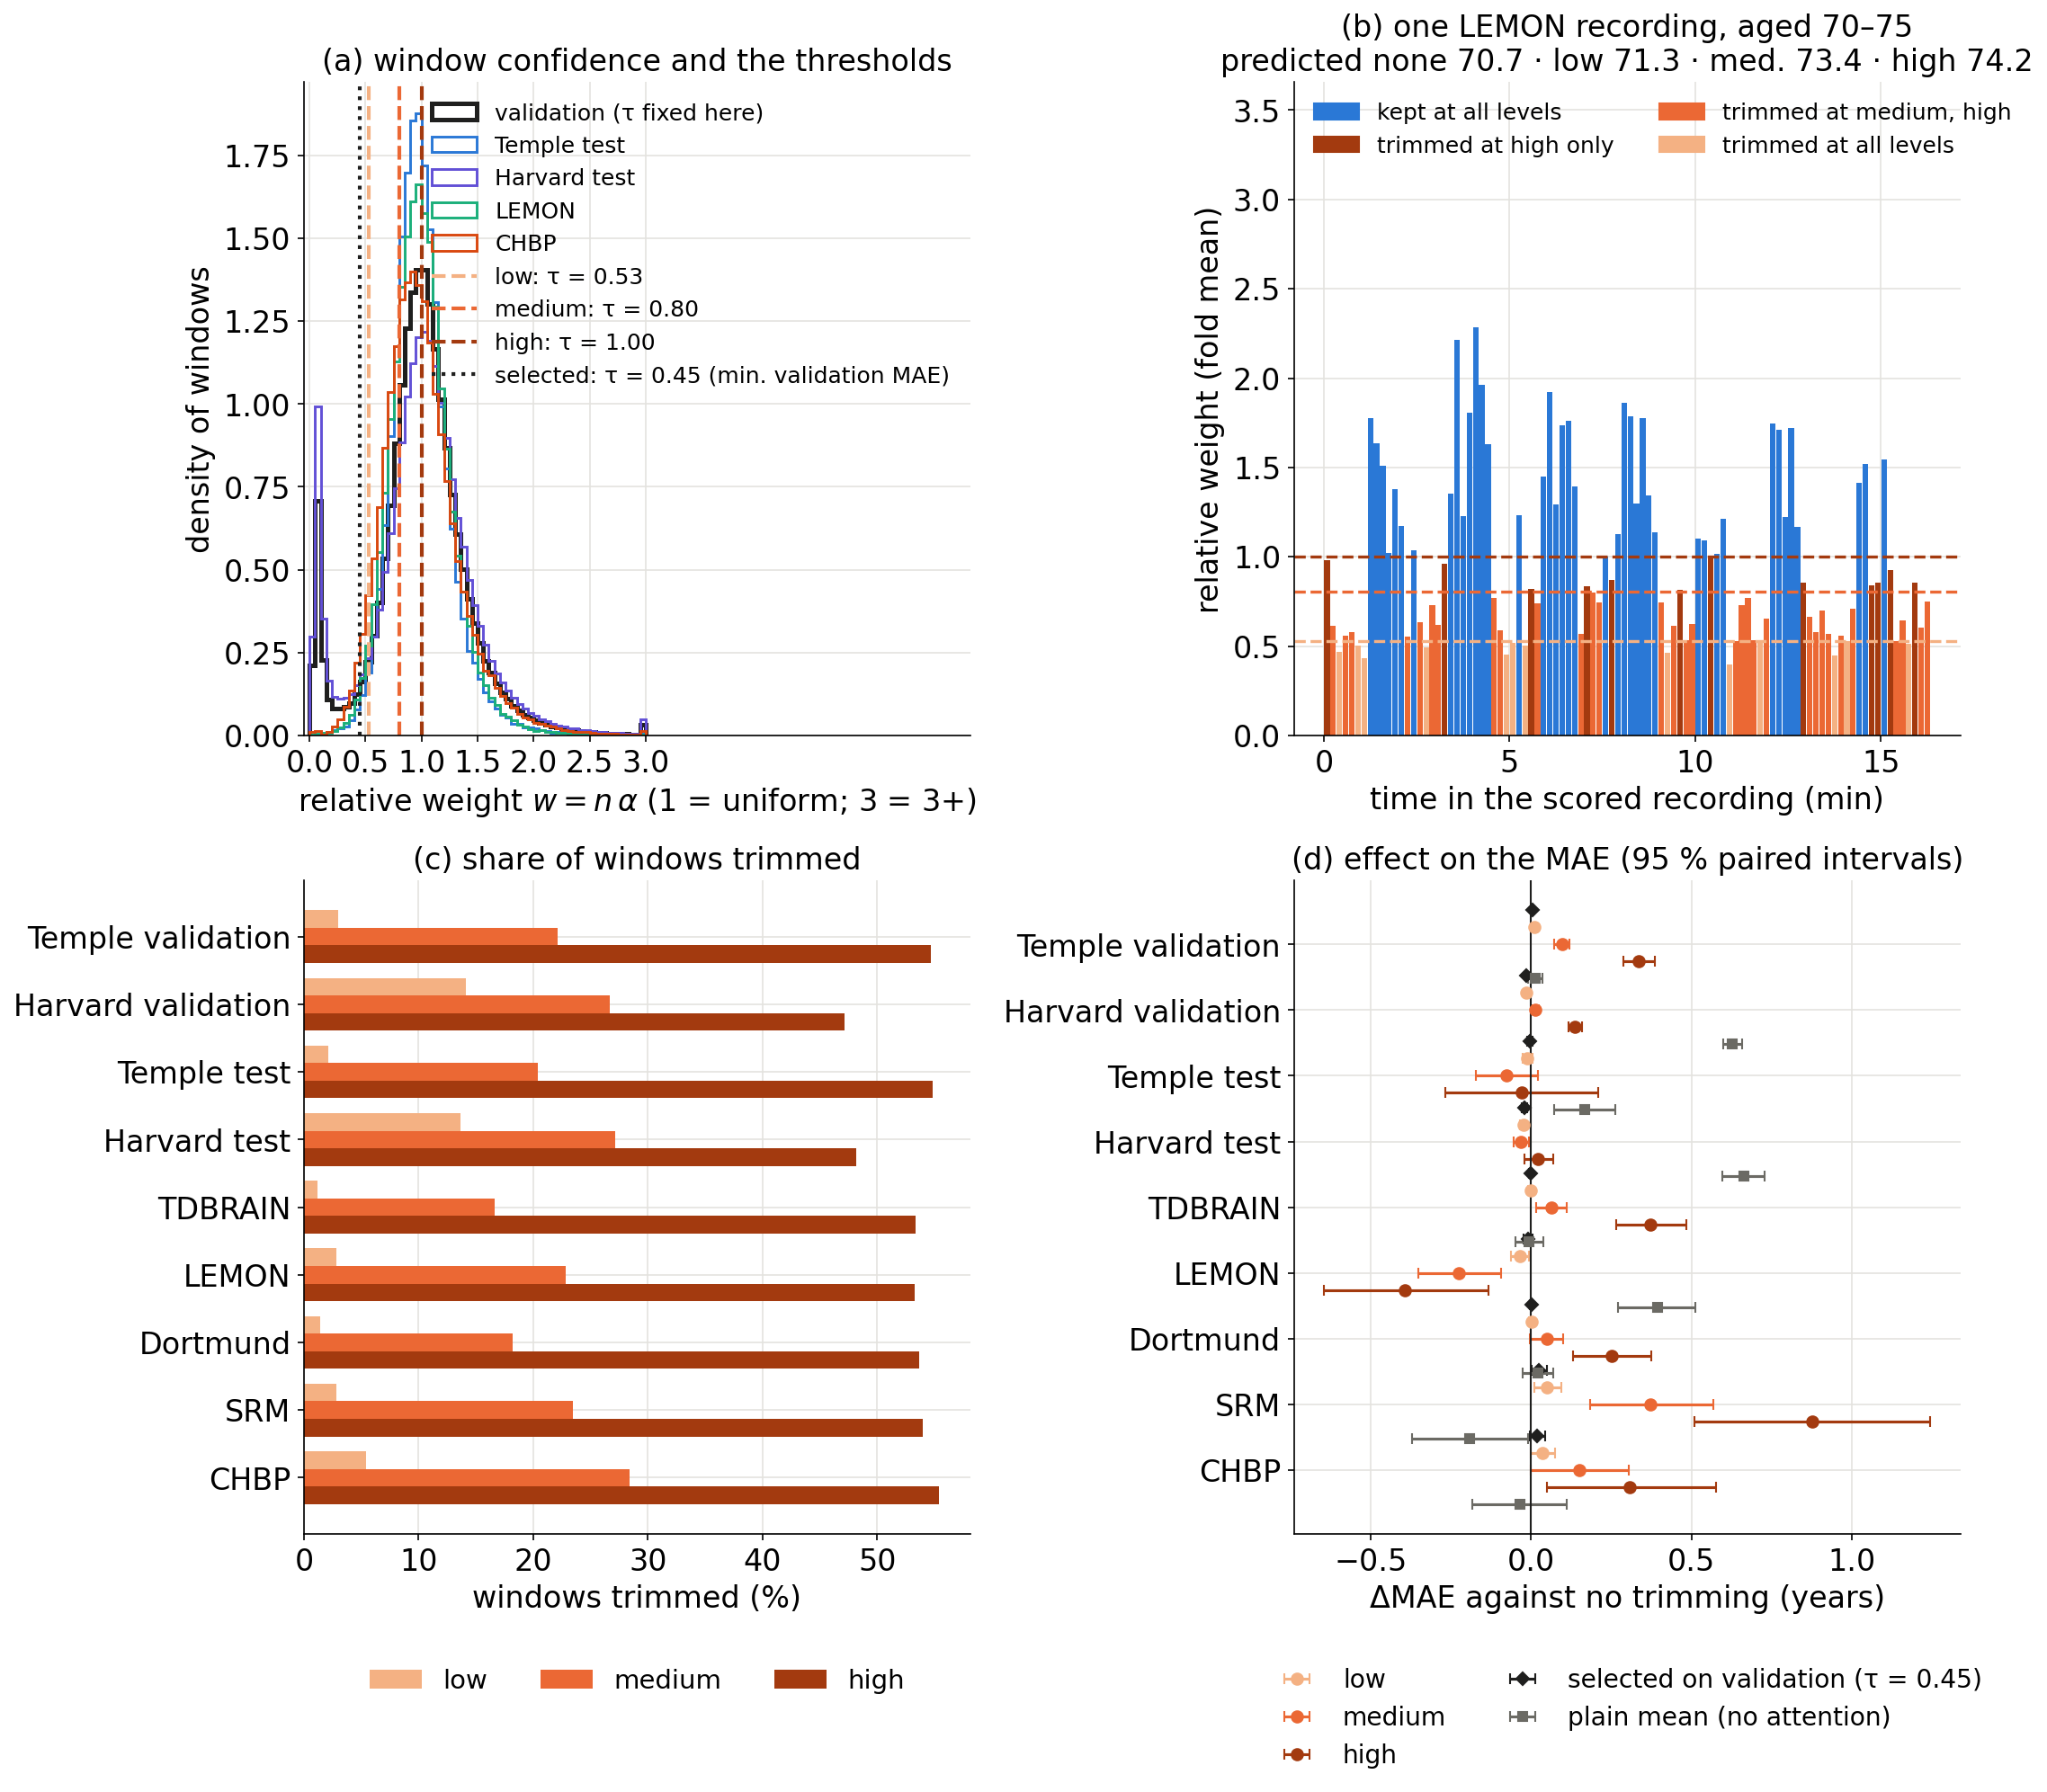
\includegraphics[width=\textwidth,height=0.62\textheight,keepaspectratio]{fig_window_trimming.png}
\caption{Window trimming by attention weight, P4. (a) Distribution of the relative attention weight $w$ per window on validation (black; the thresholds are its 10th, 25th and 50th percentiles) and on four test cohorts. (b) One LEMON recording (the recording of Figure 7): the relative weight of each 10 s window, mean of the five fold models, coloured by the level at which it is trimmed, with the ensemble prediction at each level. (c) Share of windows trimmed per cohort. (d) Change of the MAE against no trimming with 95 \% paired bootstrap intervals; grey: the plain mean of the windows instead of attention.}
\end{figure}


\begin{itemize}
\item \textbf{On validation, trimming does not help.} Low trimming changes the MAE by 0.01 years in either direction; medium and high make it worse, by up to 0.34 years in Temple and 0.14 in Harvard. The threshold selected on validation, $\tau = 0.45$, drops 1 to 3 \% of the windows (12 \% in Harvard, where a group of windows gets almost no weight, Figure 19(a)) and changes the test MAE by at most 0.03 years; low trimming by at most 0.05 years.
\item \textbf{The attention pool has already done the work.} The windows below the low threshold carry little weight in the pool, so dropping them hardly moves the prediction; dropping windows of ordinary weight (medium, high) throws away information. The pool itself matters where windows are bad: the plain mean is 0.63 to 0.66 years worse in Harvard (validation and test), 0.17 in the Temple test and 0.39 on LEMON, no different on TDBRAIN, Dortmund and CHBP, and 0.19 years better on SRM (Figure 17: on these four the weight carries no information about the window).
\item \textbf{LEMON is the exception, and it does not transfer.} High trimming lowers LEMON's MAE from 4.67 to 4.28 years [$-$0.64, $-$0.13], but raises it on TDBRAIN (+0.37), Dortmund (+0.25), CHBP (+0.31) and most on SRM (+0.87). Trimming also makes every external cohort's predictions younger (high: the bias falls by 0.3 to 1.2 years); on LEMON the MAE improves although the bias grows from $-$0.76 to $-$1.47 years, so the gain there comes from fewer large errors, not from the bias.
\item \textbf{Recommendation.} Keep the attention-pooled prediction without trimming; to discard unreliable data, set whole recordings aside by the combined score (Table 16), which lowers the MAE on every cohort.
\end{itemize}

\subsection{Age bias and its correction}

\begin{table}[t]
\centering
\small
\caption{P4 ensemble under each correction, by cohort and subset: MAE in years / slope of the prediction on age (1 = no compression). Every correction is fitted once on normal-report validation recordings (Section 10.1) and applied unchanged to every subset. For the two corrections that use the true age the first number is the mean absolute corrected gap, not an accuracy.}
\resizebox{\textwidth}{!}{%
\begin{tabular}{llllllll}
\toprule
\textbf{cohort} & \textbf{subset} & \textbf{n} & \textbf{none} & \textbf{Cole inversion, Eq. (17)} & \textbf{recalibration, Eq. (17)} & \textbf{linear gap, Eq. (18)} & \textbf{quadratic gap, Eq. (18)} \\
\midrule
Temple & all & 272 & 5.87 / 0.79 & 6.74 / 1.00 & 5.89 / 0.78 & 5.34 / 1.00 & 5.15 / 1.02 \\
 & normal report & 149 & 4.52 / 0.83 & 5.56 / 1.05 & 4.54 / 0.83 & 4.41 / 1.04 & 4.29 / 1.04 \\
 & abnormal report & 123 & 7.50 / 0.67 & 8.16 / 0.84 & 7.52 / 0.66 & 6.47 / 0.88 & 6.20 / 0.93 \\
Harvard & all & 7,338 & 5.94 / 0.83 & 7.14 / 1.04 & 5.96 / 0.82 & 5.66 / 1.03 & 5.57 / 1.05 \\
 & normal report & 1,518 & 5.69 / 0.83 & 6.94 / 1.05 & 5.72 / 0.83 & 5.51 / 1.04 & 5.35 / 1.04 \\
 & abnormal report & 2,253 & 6.49 / 0.78 & 7.68 / 0.99 & 6.51 / 0.77 & 6.09 / 0.99 & 6.04 / 1.01 \\
 & no report & 3,567 & 5.70 / 0.84 & 6.88 / 1.06 & 5.71 / 0.83 & 5.45 / 1.05 & 5.36 / 1.06 \\
TDBRAIN & all & 1,113 & 4.92 / 0.89 & 6.61 / 1.12 & 4.90 / 0.88 & 5.24 / 1.09 & 5.14 / 1.07 \\
 & healthy controls & 179 & 4.96 / 0.88 & 7.10 / 1.11 & 4.95 / 0.87 & 5.63 / 1.09 & 5.37 / 1.06 \\
 & patients & 934 & 4.92 / 0.89 & 6.52 / 1.12 & 4.89 / 0.88 & 5.17 / 1.09 & 5.09 / 1.07 \\
LEMON & all, healthy & 214 & 4.67 / 0.83 & 6.15 / 1.05 & 4.71 / 0.82 & 4.87 / 1.04 & 4.58 / 1.02 \\
Dortmund & all, healthy & 816 & 4.53 / 0.85 & 5.61 / 1.07 & 4.50 / 0.84 & 4.45 / 1.05 & 4.45 / 1.03 \\
SRM & all, healthy & 152 & 4.84 / 0.88 & 7.13 / 1.11 & 4.81 / 0.87 & 5.65 / 1.09 & 5.53 / 1.03 \\
CHBP & all, healthy & 250 & 7.95 / 0.53 & 8.99 / 0.67 & 7.99 / 0.53 & 7.13 / 0.74 & 7.26 / 0.65 \\
\bottomrule
\end{tabular}
}
\end{table}


\textbf{The models and what is applied to each dataset.} Tables 13 and 23 compare five models, and Tables 19, 20 and 23 add corrections and a sixth, device-robust model. Table 20 summarises how each model was trained and how it turns window predictions into one age; Table 21 summarises what is done for each dataset: which windows are scored, what the scoring unit is, which subsets are reported, and which corrections and rejection rules are available. Three rules hold for every table. (i) All models are trained on the training split of Temple + Harvard only (\texttt{tuh\_heedb\_v1}, 84,891 recordings, Table 5) and select their epoch on validation recordings; no test cohort is used to fit, tune, select or calibrate anything. (ii) The accuracy tables (Tables 13 and 23) score the raw prediction, without any age-bias correction and without rejection. (iii) A correction is always fitted on the normal-report adult validation recordings of the training cohort (Eq. (30), Section 10.1) and applied unchanged to every test cohort and subset (Tables 19, 20); a rejection threshold is the cohort's own 80 \% score quantile (Tables 16, 20), or a threshold fixed on validation (Section 10.4).

\begin{table}[t]
\centering
\small
\caption{The models compared. Training data, input preprocessing and target are those of Tables 4 and 5 for every model; the rows differ in initialisation, schedule, pooling of the windows and ensembling. GPU hours on one A10G.}
\resizebox{\textwidth}{!}{%
\begin{tabular}{llllll}
\toprule
\textbf{model} & \textbf{initialisation and schedule} & \textbf{pooling of the windows} & \textbf{ensemble and selection} & \textbf{cost} & \textbf{rejection score} \\
\midrule
E2L, window model (Section 4.2) & LaBraM base checkpoint; 16 epochs (4 warm-up), batch 512 at lr $4 \times 10^{-4}$ for epochs 1--6, then batch 256 at $2.8 \times 10^{-4}$; 5 minutes of every recording per epoch; Huber loss on the z-scored age, mixup & plain mean of the window predictions, Eq. (9) & one model, epoch 11 selected on validation & 26.6 h & spread of the window predictions \\
L1, two-step attention & E2L's epoch-11 checkpoint plus 4 bag epochs: bags of 8 windows, 32 recordings per step, lr $10^{-4}$, encoder frozen in the first bag epoch, pool and head at 5 $\times$ the lr & attention pool, Eq. (10) & one model, epoch selected on validation & +1.1 h & none (windows not saved for every cohort) \\
W4, two-step gated attention & as L1 & gated attention pool (tanh and sigmoid branches)~\citep{ilse2018abmil} & as L1 & +1.1 h & none \\
P3 ensemble (Section 4.3) & LaBraM base checkpoint; one run of 17 epochs in three phases (window, attention only, joint), learning rate restarted for the joint phase, retention term 0.1 (Table 11) & attention pool, Eq. (10) & 5 fold models of a patient-grouped cross-validation (Section 3.3), each selecting its epoch on its own validation fold; prediction = mean of the five, Eq. (12) & 12.5 h per fold & spread, total (Eq. (14)), learned \\
P4 ensemble, the main model & as P3, but one cosine schedule over all 17 epochs, per-window loss 0.5 in the joint phase, every recording drawn twice per epoch (Table 11) & attention pool, Eq. (10) & as P3 & 12.8 h per fold & spread, total, learned \\
device-robust E2L (Section 6.5) & E2L's recipe from the LaBraM base checkpoint, with the input band-limited to 1--45 Hz (Eq. (26)) and every window scaled to a fixed amplitude (Eq. (27)) in training and at test; early-stopped after epoch 14 & plain mean, Eq. (9) & one model, epoch 9 selected on validation & as E2L & spread \\
\bottomrule
\end{tabular}
}
\end{table}


\begin{table}[t]
\centering
\small
\caption{What is applied to each dataset. \texttt{windows}: which 10 s windows of a recording are scored; \texttt{unit}: what one prediction and one error refer to; \texttt{subsets}: the groups reported separately (Tables 13, 14, 20). Every dataset is scored by the five models of Tables 13 and 23 with the raw prediction, and with the four corrections of Eqs. (17) and (18) fitted on the training cohort's validation recordings; the ensembles also with the 20 \% rejection.}
\resizebox{\textwidth}{!}{%
\begin{tabular}{llllll}
\toprule
\textbf{dataset} & \textbf{role} & \textbf{windows} & \textbf{unit} & \textbf{subsets} & \textbf{specific to the dataset} \\
\midrule
Temple & in-domain test (TUAB evaluation split, adults) & first 5 minutes after a 60 s trim at each end (the training protocol) & recording & normal / abnormal report & patients never in training or validation (Section 3.3) \\
Harvard & in-domain test (held-out patients) & as Temple & recording & normal / abnormal / no report & half of the recordings have no report verdict \\
TDBRAIN & zero-shot & every window, no trim (2-minute files) & session: mean of its eyes-closed and eyes-open file & healthy controls / patients & aggregates only (data use agreement) \\
LEMON & zero-shot & every window after a 60 s trim at each end & recording & all healthy & ages known only as 5-year bins (midpoint used) \\
Dortmund & zero-shot, kept test-only & every window, no trim (3-minute runs) & session: mean of its four runs & all healthy & 208 people recorded twice (Section 6.7) \\
SRM & zero-shot & every window, no trim (4-minute files) & recording & all healthy & the smallest report cohort \\
CHBP & zero-shot, the recording-chain case & every window after a 60 s trim at each end & recording & all healthy & recorded 0.5--50 Hz at about 0.6 $\times$ the training amplitude: the device-robust E2L is the model chosen for it (Table 27); test-time fixes in Table 27 change only CHBP's signals, never the model \\
\bottomrule
\end{tabular}
}
\end{table}


Table 22 lists the configuration settings of the six models side by side, read from the configuration files saved with each run; the full list of fields on which they differ is in \texttt{docs/data/external\_eval/tech\_report/config\_comparison.csv} (\texttt{scripts/report\_config\_table.py}). Every model shares the rest: the LaBraM base encoder (12 blocks, width 200) with a class-token readout, a linear head and drop-path 0.1; the 19 channels of the 10--20 system (A1, A2, T1, T2 dropped) with a common average reference, in 10 s windows; AdamW with weight decay 0.05 and layer-wise learning-rate decay 0.65; the Huber loss ($\delta = 1$) on the z-scored age with mixup ($\alpha = 0.4$); 60 s trimmed at each end of a recording, and validation on its first 5 minutes.

\begin{table}[t]
\centering
\small
\caption{Configuration settings on which the models differ. Learning rates are peak values of a cosine schedule with linear warm-up; \texttt{bag} = 8 windows of one recording; \texttt{pool + head lr} = learning-rate multiplier of the attention pool and the head.}
\resizebox{\textwidth}{!}{%
\begin{tabular}{lllllll}
\toprule
\textbf{setting} & \textbf{E2L} & \textbf{L1} & \textbf{W4} & \textbf{P3} & \textbf{P4} & \textbf{device-robust E2L} \\
\midrule
initial weights & LaBraM base & E2L, epoch 11 & E2L, epoch 11 & LaBraM base & LaBraM base & LaBraM base \\
extra input processing & none & none & none & none & none & band 1--45 Hz, window amplitude normalised \\
epochs (warm-up) & 16 (4) & 4 (1) & 4 (1) & 17 (3) & 17 (3) & 16 (4) \\
batch & 512 windows (epochs 1--6), then 256 & 32 bags & 32 bags & window phase 256 windows, then 32 bags & as P3 & 256 windows \\
peak lr & $4 \times 10^{-4}$, then $2.8 \times 10^{-4}$ & $10^{-4}$ & $10^{-4}$ & $2.8 \times 10^{-4}$; bag phase restarts at $10^{-4}$ & $2.8 \times 10^{-4}$, one schedule & $2.8 \times 10^{-4}$ \\
training sample per recording and epoch & 5 minutes & 1 bag & 1 bag & window phase 4 draws of 8 windows, then 1 bag & as P3, then 2 bags & 5 minutes \\
phases (epochs) & windows only & bags only & bags only & window 0--9, attention only 10, joint 11--16 & window 0--7, attention only 8, joint 9--16 & windows only \\
encoder frozen & -- & first epoch & first epoch & attention-only epoch (head frozen too) & as P3 & -- \\
pool, pool + head lr & mean of windows & attention, $\times$ 5 & gated attention, $\times$ 5 & attention, $\times$ 5 & attention, $\times$ 5 & mean of windows \\
extra loss terms & -- & attention entropy 0.01 & attention entropy 0.01 & entropy 0.01, retention 0.1 & entropy 0.01, per-window 0.5 & -- \\
cross-validation & -- & -- & -- & 5 folds, test held out & 5 folds, test held out & -- \\
selection & early stopping on validation (patience 5): epoch 11 & best validation epoch & best validation epoch & each fold's best epoch on its own validation fold & as P3 & early stopping: epoch 9 \\
\bottomrule
\end{tabular}
}
\end{table}


\begin{table}[t]
\centering
\small
\caption{MAE in years and, in brackets, the mean gap (bias) by age group and model, raw predictions. In-domain: the Temple and Harvard test recordings; external: the four zero-shot cohorts of volunteers and outpatients pooled (TDBRAIN and Dortmund as sessions). Models as in Table 13. Bold: the best model of the row. Per-cohort values: \texttt{docs/data/external\_eval/tech\_report/age\_groups.csv}.}
\resizebox{\textwidth}{!}{%
\begin{tabular}{llllllll}
\toprule
\textbf{set} & \textbf{age} & \textbf{n} & \textbf{E2L} & \textbf{L1} & \textbf{W4} & \textbf{P3 ens.} & \textbf{P4 ens.} \\
\midrule
Temple + Harvard & 18--29 & 1,246 & 7.43 (+7.2) & 4.39 (+3.2) & 4.42 (+3.4) & \textbf{4.25} (+3.2) & 4.32 (+3.5) \\
 & 30--39 & 846 & 6.24 (+4.7) & 6.03 (+2.6) & \textbf{5.95} (+2.6) & 5.98 (+2.5) & 5.98 (+2.8) \\
 & 40--49 & 899 & \textbf{6.35} (+2.8) & 6.64 (+2.2) & 6.67 (+2.2) & 6.64 (+2.2) & 6.57 (+2.5) \\
 & 50--59 & 1,212 & \textbf{5.54} (+0.7) & 6.12 (+1.5) & 6.15 (+1.5) & 6.07 (+1.7) & 5.91 (+1.7) \\
 & 60--69 & 1,456 & 5.73 ($-$2.6) & 6.04 ($-$0.6) & 6.06 ($-$0.6) & 5.93 ($-$0.4) & \textbf{5.64} ($-$0.6) \\
 & 70+ & 1,951 & 9.20 ($-$8.8) & 6.94 ($-$5.3) & 6.96 ($-$5.3) & \textbf{6.75} ($-$5.2) & 6.90 ($-$5.8) \\
 & all & 7,610 & 7.00 ($-$0.6) & 6.08 ($-$0.1) & 6.10 ($-$0.1) & 5.98 ($-$0.1) & \textbf{5.94} ($-$0.1) \\
TDBRAIN, LEMON, Dortmund, SRM & 18--29 & 554 & 3.39 (+2.0) & 3.19 (+0.4) & 3.10 (+0.6) & \textbf{3.02} (+0.7) & 3.09 (+1.5) \\
 & 30--39 & 413 & \textbf{4.47} ($-$0.0) & 5.20 ($-$0.3) & 4.97 ($-$0.7) & 4.71 ($-$0.5) & 4.57 (+0.2) \\
 & 40--49 & 403 & 5.58 ($-$0.9) & 5.92 ($-$0.2) & 5.98 ($-$0.8) & 5.68 ($-$0.6) & \textbf{5.42} ($-$0.2) \\
 & 50--59 & 459 & 5.61 ($-$3.3) & 5.48 ($-$1.6) & 5.72 ($-$2.3) & 5.38 ($-$2.0) & \textbf{5.03} ($-$1.9) \\
 & 60--69 & 331 & 6.61 ($-$5.1) & 6.05 ($-$2.6) & 6.05 ($-$3.1) & 6.08 ($-$3.5) & \textbf{5.71} ($-$3.7) \\
 & 70+ & 135 & 8.50 ($-$8.0) & \textbf{6.53} ($-$4.7) & 6.70 ($-$5.0) & 6.73 ($-$5.3) & 6.86 ($-$6.0) \\
 & all & 2,295 & 5.18 ($-$1.6) & 5.10 ($-$1.0) & 5.10 ($-$1.3) & 4.92 ($-$1.2) & \textbf{4.75} ($-$0.9) \\
\bottomrule
\end{tabular}
}
\end{table}


\begin{table}[t]
\centering
\small
\caption{P4 ensemble by age group: MAE in years and, in brackets, the mean gap, without correction, with the corrections of Eqs. (17) and (18) fitted on validation, and after rejecting the 20 \% least confident units of each cohort by the total score of Eq. (14) (threshold over the whole cohort; in brackets the share of the age group that is kept). Quadratic gap: mean absolute corrected gap, uses the true age. Sets as in Table 23.}
\resizebox{\textwidth}{!}{%
\begin{tabular}{llllllll}
\toprule
\textbf{set} & \textbf{age} & \textbf{n} & \textbf{none} & \textbf{Cole inversion} & \textbf{recalibration} & \textbf{quadratic gap} & \textbf{20 \% rejected: MAE (kept)} \\
\midrule
Temple + Harvard, all & 18--29 & 1,246 & 4.32 (+3.5) & 5.88 ($-$2.0) & 4.51 (+3.9) & 4.04 ($-$0.4) & 3.33 (91 \%) \\
 & 30--39 & 846 & 5.98 (+2.8) & 7.62 (+0.1) & 5.98 (+3.1) & 6.08 ($-$0.3) & 5.25 (83 \%) \\
 & 40--49 & 899 & 6.57 (+2.5) & 8.14 (+2.4) & 6.56 (+2.7) & 6.34 (+0.8) & 6.07 (75 \%) \\
 & 50--59 & 1,212 & 5.91 (+1.7) & 7.98 (+4.0) & 5.88 (+1.8) & 6.02 (+2.1) & 5.69 (72 \%) \\
 & 60--69 & 1,456 & 5.64 ($-$0.6) & 7.82 (+3.7) & 5.60 ($-$0.6) & 6.08 (+2.5) & 5.24 (74 \%) \\
 & 70+ & 1,951 & 6.90 ($-$5.8) & 6.19 (+0.6) & 6.90 ($-$5.8) & 5.25 (+2.1) & 6.23 (84 \%) \\
 & all & 7,610 & 5.94 ($-$0.1) & 7.12 (+1.4) & 5.96 ($-$0.0) & 5.55 (+1.4) & 5.31 (80 \%) \\
Temple + Harvard, normal report & 18--29 & 389 & 4.43 (+3.6) & 6.22 ($-$2.0) & 4.62 (+3.9) & 4.25 ($-$0.3) & 3.72 (95 \%) \\
 & 30--39 & 248 & 5.05 (+1.8) & 6.65 ($-$1.1) & 5.04 (+2.1) & 5.35 ($-$1.3) & 4.66 (89 \%) \\
 & 40--49 & 203 & 5.99 (+0.8) & 7.49 (+0.3) & 5.96 (+1.0) & 5.99 ($-$0.9) & 5.63 (86 \%) \\
 & 50--59 & 282 & 5.62 (+0.8) & 7.53 (+2.9) & 5.58 (+1.0) & 5.75 (+1.2) & 5.44 (84 \%) \\
 & 60--69 & 261 & 5.73 ($-$1.7) & 7.18 (+2.1) & 5.68 ($-$1.6) & 5.58 (+1.3) & 5.40 (82 \%) \\
 & 70+ & 284 & 7.20 ($-$6.3) & 6.27 ($-$0.3) & 7.20 ($-$6.3) & 5.21 (+1.3) & 6.82 (90 \%) \\
 & all & 1,667 & 5.59 ($-$0.0) & 6.82 (+0.2) & 5.61 (+0.2) & 5.25 (+0.3) & 5.15 (88 \%) \\
Temple + Harvard, abnormal report & 18--29 & 283 & 5.58 (+4.9) & 6.54 ($-$0.2) & 5.78 (+5.2) & 4.81 (+1.0) & 3.77 (82 \%) \\
 & 30--39 & 177 & 7.53 (+5.1) & 8.65 (+3.0) & 7.59 (+5.4) & 6.77 (+2.0) & 7.12 (68 \%) \\
 & 40--49 & 230 & 8.04 (+5.2) & 9.89 (+5.8) & 8.06 (+5.3) & 7.44 (+3.5) & 6.92 (58 \%) \\
 & 50--59 & 345 & 6.37 (+2.5) & 8.69 (+5.1) & 6.36 (+2.6) & 6.50 (+3.0) & 6.16 (61 \%) \\
 & 60--69 & 519 & 5.77 ($-$0.2) & 8.23 (+4.2) & 5.73 ($-$0.2) & 6.40 (+3.0) & 5.28 (69 \%) \\
 & 70+ & 822 & 6.81 ($-$5.4) & 6.55 (+1.0) & 6.81 ($-$5.4) & 5.53 (+2.5) & 6.13 (83 \%) \\
 & all & 2,376 & 6.54 ($-$0.1) & 7.70 (+2.8) & 6.56 (+0.0) & 6.05 (+2.6) & 5.77 (73 \%) \\
TDBRAIN, LEMON, Dortmund, SRM & 18--29 & 554 & 3.09 (+1.5) & 5.69 ($-$4.3) & 3.18 (+1.8) & 3.83 ($-$2.4) & 2.69 (92 \%) \\
 & 30--39 & 413 & 4.57 (+0.2) & 6.68 ($-$3.2) & 4.52 (+0.5) & 5.43 ($-$2.9) & 4.34 (86 \%) \\
 & 40--49 & 403 & 5.42 ($-$0.2) & 6.92 ($-$0.9) & 5.37 ($-$0.0) & 5.67 ($-$1.8) & 5.67 (74 \%) \\
 & 50--59 & 459 & 5.03 ($-$1.9) & 6.11 ($-$0.5) & 4.96 ($-$1.8) & 4.94 ($-$1.5) & 4.79 (70 \%) \\
 & 60--69 & 331 & 5.71 ($-$3.7) & 6.14 ($-$0.3) & 5.65 ($-$3.6) & 4.86 ($-$0.7) & 5.14 (73 \%) \\
 & 70+ & 135 & 6.86 ($-$6.0) & 5.94 ($-$0.7) & 6.84 ($-$6.0) & 4.78 (+0.3) & 6.29 (79 \%) \\
 & all & 2,295 & 4.75 ($-$0.9) & 6.25 ($-$2.0) & 4.73 ($-$0.7) & 4.87 ($-$1.8) & 4.39 (80 \%) \\
\bottomrule
\end{tabular}
}
\end{table}


\begin{figure}[t]
\centering
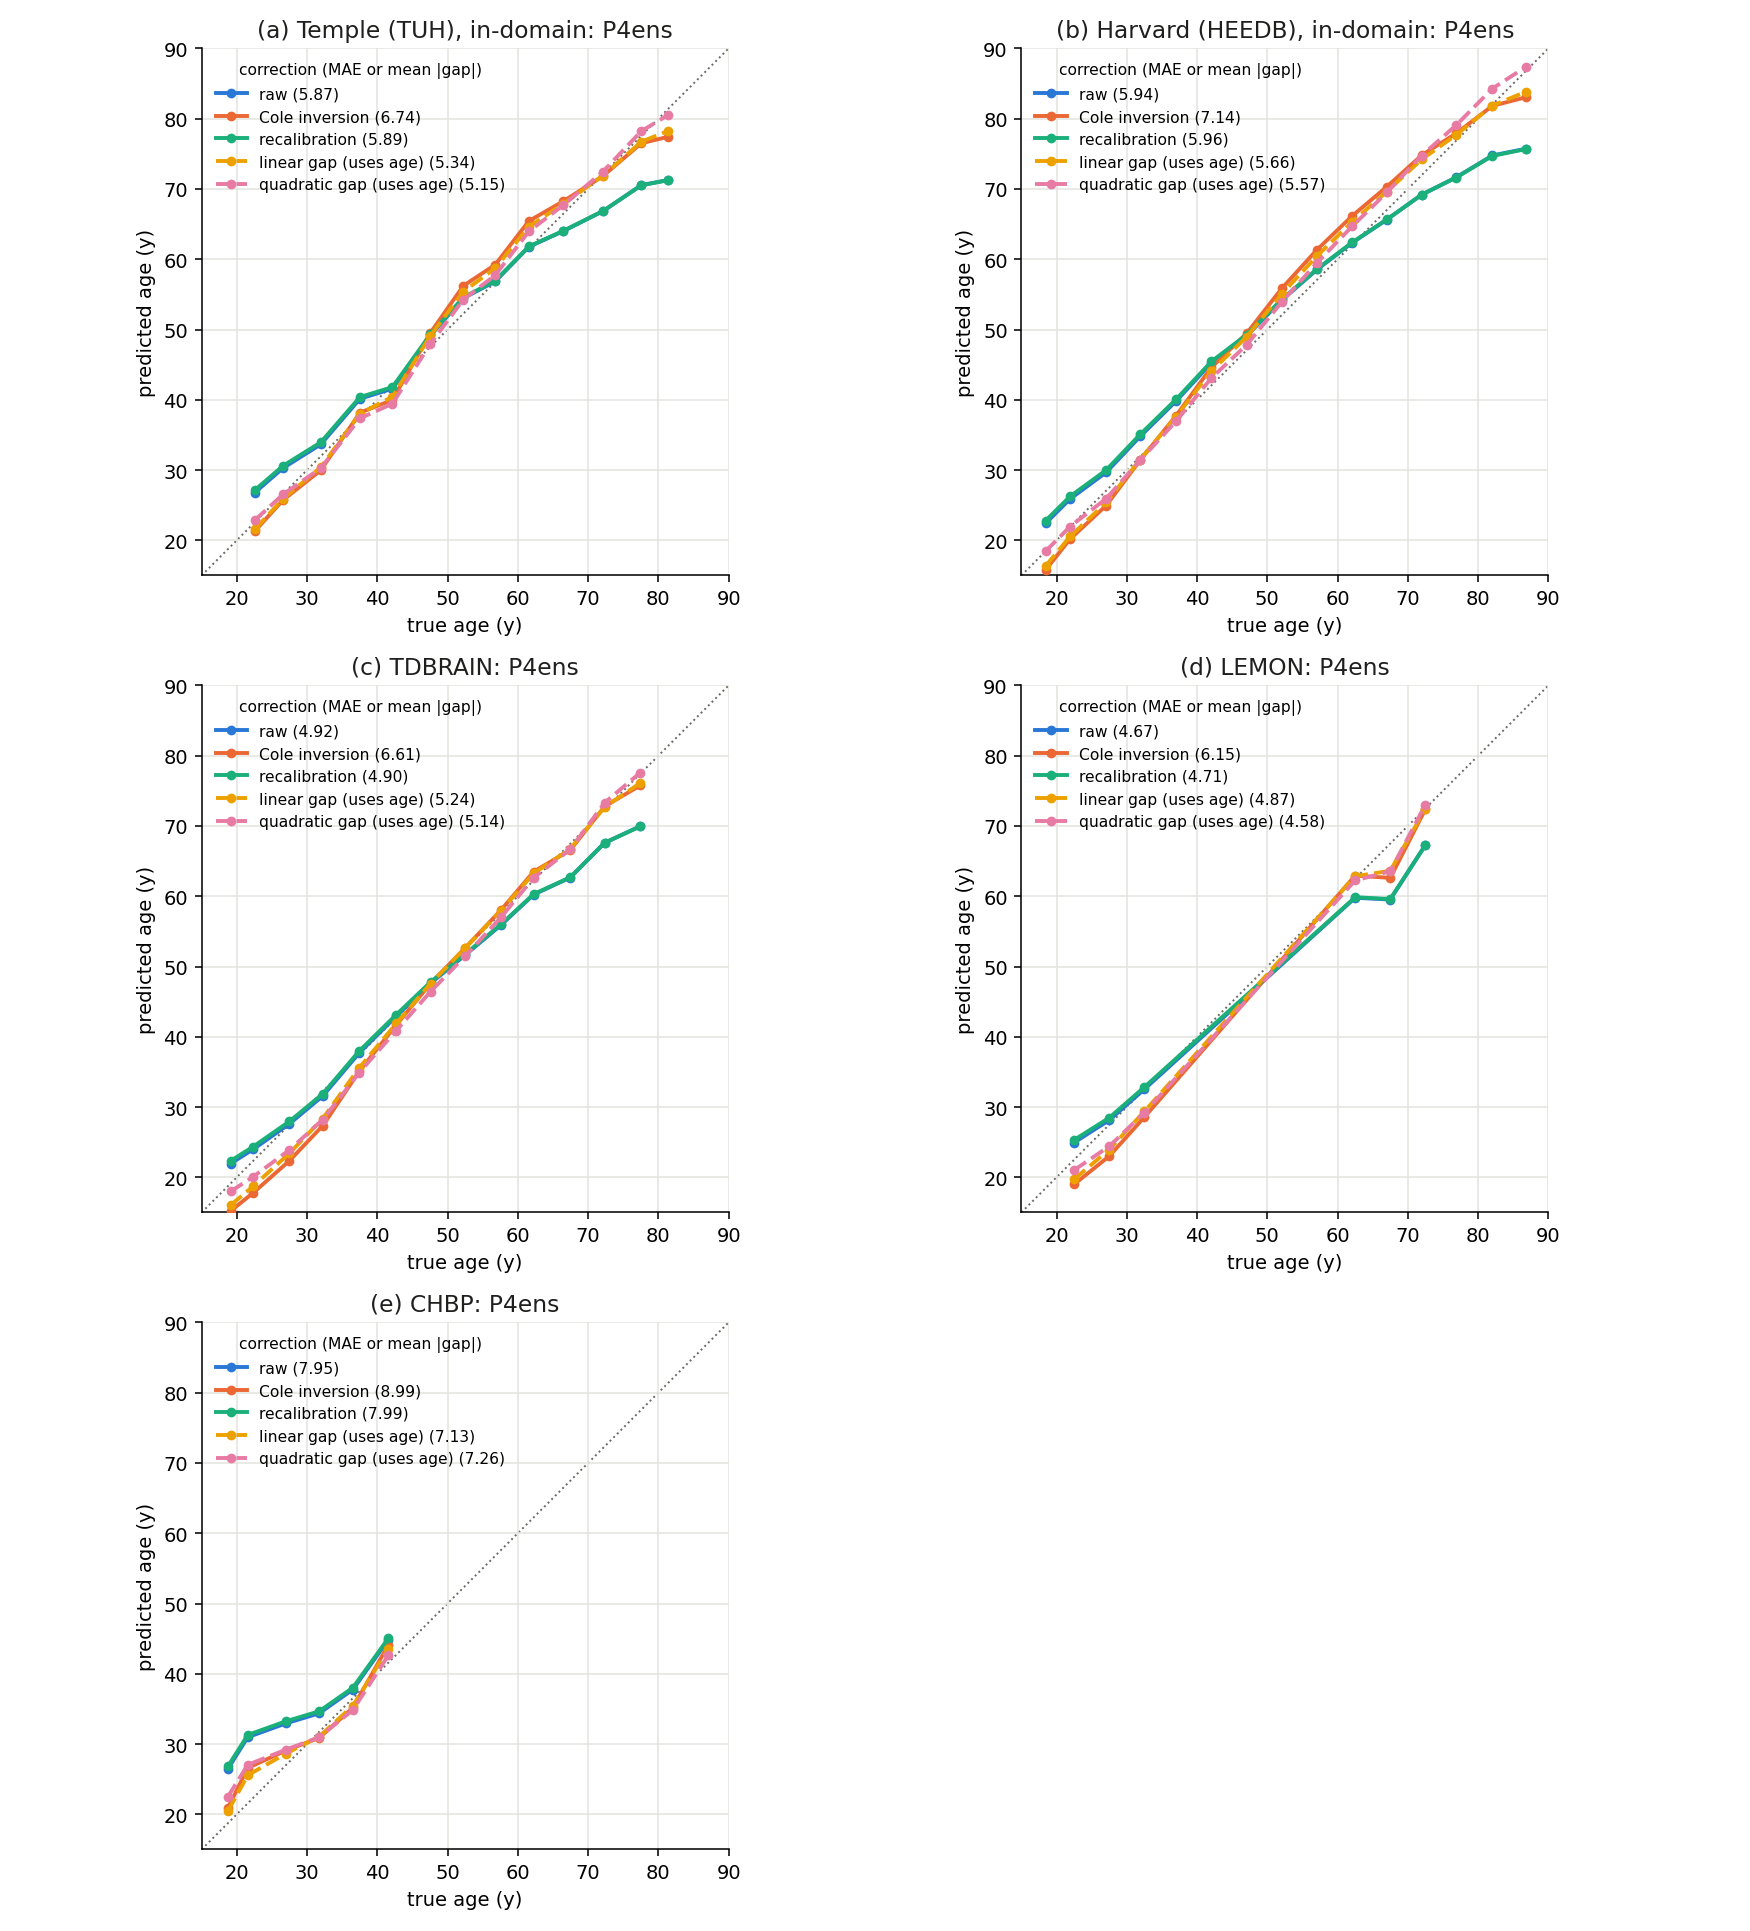
\includegraphics[width=\textwidth,height=0.62\textheight,keepaspectratio]{pred_vs_age_corrections.png}
\caption{Predicted against true age per cohort for the P4 ensemble under each correction (means per 5-year age bin). Solid: corrections that need no true age. Dashed: corrections that use it.}
\end{figure}


The ensembles compress less than the window model: in-domain slopes are 0.79 to 0.84 against 0.70 to 0.72 for E2L. A correction fitted on validation data transfers to the external cohorts that resemble the training data (slope 1.00 to 1.12 after correction) but not to CHBP. Removing the bias without the true age costs accuracy: Cole inversion raises the MAE by 0.9 to 2.3 years, because it scales the prediction noise by $1/a$, and recalibration changes nothing. The raw prediction is therefore the best age estimate, and the corrections serve the analysis of the gap. After correction, recordings with an abnormal report look 1.8 to 4.2 years older than those with a normal report in Temple and Harvard ($p \le 0.002$ with every model); before correction the difference is hidden by the age confound. In TDBRAIN the corrected difference between patients and controls is 0.4 to 1.1 years and not significant.

What Tables 19, 23 and 24 add:

\begin{itemize}
\item \textbf{Normal against abnormal (Table 19).} The abnormal subsets are compressed more than the normal ones (slope 0.67 against 0.83 in Temple, 0.78 against 0.83 in Harvard). A correction fitted on normal-report validation recordings brings the normal subsets to a slope of 1.04 to 1.05 and leaves Temple's abnormal subset under-corrected (0.84 to 0.93). The gap corrections lower the mean absolute corrected gap most in the abnormal subsets (Temple 7.50 to 6.20 years with the quadratic form), because those patients are older and so carry more of the age trend. In TDBRAIN, controls and patients behave alike under every correction.
\item \textbf{Age groups (Table 23).} Every model over-predicts the young and under-predicts the old. The window model E2L does so most: +7.2 years at 18--29 and $-$8.8 years from 70 in-domain. The attention models halve the young offset (+3.2 to +3.5 years) and reduce the old one to $-$5.2 to $-$5.8 years, which is where most of their gain over E2L comes from. Near the middle of the training age distribution, 40--59 years, E2L is as good as or better than the attention models in-domain, because the error of a compressed model is smallest near the mean. The two-step attention models L1 and W4 are within 0.1 years of each other in every age group; the P4 ensemble is best in most groups from 40 years on in the external cohorts.
\item \textbf{Corrections by age (Table 24).} Cole inversion removes the age trend of the bias (from 70: $-$5.8 to +0.6 years in-domain) but raises the MAE by 1.5 to 2.5 years in every age group below 70; it helps only the oldest group. Recalibration changes neither MAE nor bias. The quadratic gap correction flattens the bias at every age but, being a residual, is not an accuracy.
\item \textbf{Rejection by age (Table 24).} The 20 \% that are set aside are not spread evenly over age: 91 to 92 \% of the 18--29-year-olds are kept, against 70 to 75 \% of the 40--69-year-olds, in-domain and externally. Among abnormal-report recordings only 58 to 69 \% of the 30--69-year-olds are kept. The kept MAE falls in every age group, most for the young (in-domain 4.32 to 3.33 years at 18--29). Rejection therefore improves the error at every age, but it also changes the age and report mix of the kept recordings, which a group comparison must account for.
\end{itemize}

\subsection{A recording-chain shift and its correction: CHBP}

CHBP is the one cohort on which every model fails. This section locates the difference in the signal, tests it causally on training-domain recordings, and compares corrections. The numbers here are for the window model E2L and its retrained variants on the first 5 minutes of each recording, the training protocol, so E2L on CHBP reads 9.55 years here and 9.35 in Table 13 (every window). No CHBP age is used anywhere.

\textbf{Where the signals differ.} Table 25 and Figure 21 compare CHBP with healthy Temple and Harvard recordings weighted to CHBP's age distribution. Two properties of the recording chain stand out. The amplitude is 0.5 to 0.6 times that of the training data. And the band is narrower: CHBP was recorded with a 0.5 Hz high-pass and a 50 Hz low-pass~\citep{valdessosa2021chbp}, so its power below 1 Hz is 6 to 12 \% and its power at 45--70 Hz 4 to 5 \% of the training data's. The alpha rhythm, in contrast, is stronger: CHBP is alert, eyes-closed, artifact-free research EEG, which should read as younger, not older. The age range is not the cause either: at CHBP's ages E2L reaches a correlation of 0.66 with age on its own domain, against 0.44 on CHBP. CHBP also holds two acquisition groups, a 64-channel cap (161 recordings; E2L MAE 7.58, r 0.55) and a 120-channel cap (89 recordings; 13.10, r 0.27) with a different spectrum.

\begin{table}[t]
\centering
\small
\caption{CHBP against healthy Temple and Harvard recordings of the same ages (150 each, normal EEG report). Medians over recordings; power in $\mu$V$^2$/Hz, common average reference.}
\begin{tabular}{llll}
\toprule
\textbf{signal feature} & \textbf{CHBP} & \textbf{Temple} & \textbf{Harvard} \\
\midrule
channel standard deviation ($\mu$V) & 5.8 & 9.9 & 12.8 \\
share of windows with a channel above 100 $\mu$V & 0.00 & 0.03 & 0.20 \\
power 0.1--1 Hz & 5.0 & 43.2 & 90.5 \\
power 1--4 Hz (delta) & 1.86 & 3.86 & 4.36 \\
power 8--13 Hz (alpha) & 1.98 & 1.05 & 0.92 \\
power 13--30 Hz (beta) & 0.159 & 0.266 & 0.244 \\
power 30--45 Hz & 0.017 & 0.069 & 0.056 \\
power 45--70 Hz & 0.001 & 0.036 & 0.028 \\
relative alpha power & 0.44 & 0.17 & 0.15 \\
aperiodic exponent & 1.70 & 1.33 & 1.42 \\
\bottomrule
\end{tabular}
\end{table}


\begin{figure}[t]
\centering
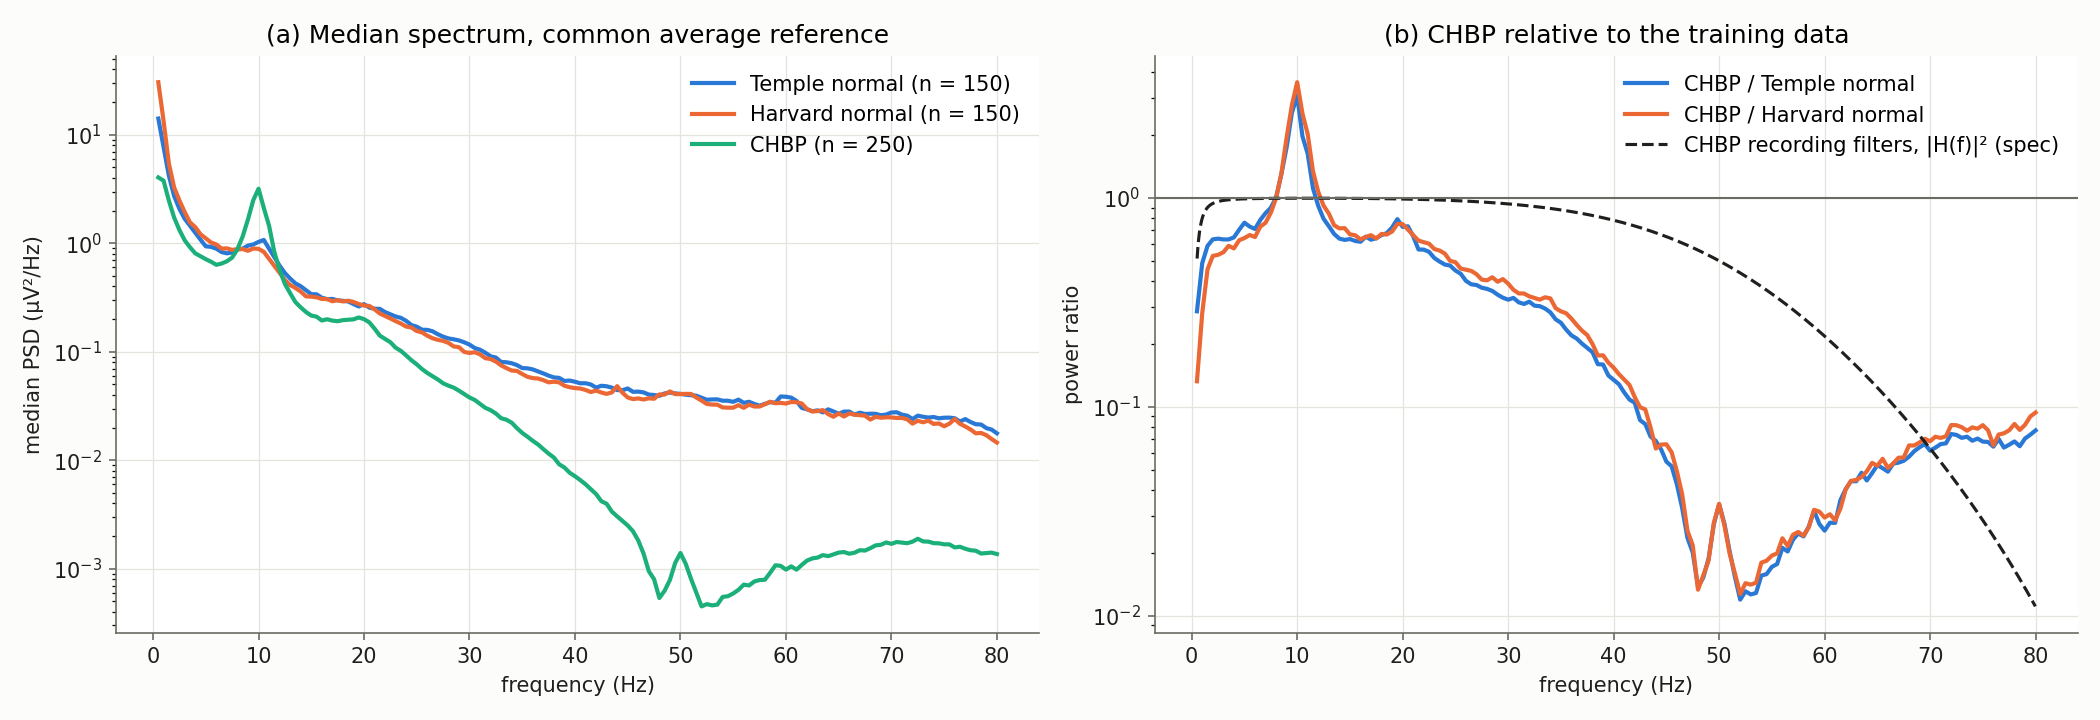
\includegraphics[width=\textwidth,height=0.62\textheight,keepaspectratio]{../figures/chbp/chbp_shift_psd.png}
\caption{(a) Median power spectrum of CHBP and of age-matched healthy Temple and Harvard recordings. (b) CHBP's spectrum divided by each reference; dashed: the power response of CHBP's recording filters as specified.}
\end{figure}


\textbf{Causal test.} The two differences are imposed on 300 healthy Temple and Harvard recordings of CHBP's ages, with a gain $k$ and zero-phase Butterworth filters $h$:

\begin{equation}
x' = k\,x, \qquad x' = h_{LP} * h_{HP} * x \tag{24}
\end{equation}

\begin{table}[t]
\centering
\small
\caption{E2L on 300 training-domain recordings made CHBP-like with Eq. (24). The sample is young, so E2L over-predicts it even without a transform.}
\begin{tabular}{llll}
\toprule
\textbf{transform} & \textbf{MAE} & \textbf{bias} & \textbf{r} \\
\midrule
none & 7.02 & +5.1 & 0.66 \\
amplitude $\times$ 0.62 & 11.34 & +10.9 & 0.66 \\
high-pass 0.5 Hz & 7.71 & +6.0 & 0.63 \\
low-pass 50 Hz & 8.04 & +3.8 & 0.40 \\
amplitude $\times$ 0.62 and band 0.5--50 Hz & 13.71 & +12.6 & 0.37 \\
\bottomrule
\end{tabular}
\end{table}


The two effects are separate (Table 26). The lower amplitude adds an offset of about 6 years and leaves the ranking intact: the model has learned that low amplitude means old. The 50 Hz low-pass leaves the offset and destroys the ranking: the model uses content above 50 Hz that CHBP does not have. Together they reproduce CHBP's result (13.7 years, r 0.37) on recordings the model otherwise predicts well.

\textbf{Corrections.} We compare two that change only the test data and four that change the training. At test time, one gain for the cohort, or spectrum matching: every channel of CHBP is filtered so that the cohort's median spectrum $\bar P$ equals that of a label-free training reference, per cap, an idea used for sleep staging~\citep{gnassounou2023cmmn}:

\begin{equation}
X'(f) = X(f)\,\operatorname{clip}\Big( \sqrt{ \bar P_{ref}(f) / \bar P_{CHBP}(f) },\ 0.1,\ 10 \Big) \tag{25}
\end{equation}

In training, the model input is band-limited to 1--45 Hz with order-8 zero-phase Butterworth responses and, optionally, every 10 s window is scaled to a fixed amplitude:

\begin{equation}
X'(f) = X(f)\,\frac{(f/f_{lo})^{16}}{1 + (f/f_{lo})^{16}}\,\frac{1}{1 + (f/f_{hi})^{16}}, \qquad f_{lo} = 1, \quad f_{hi} = 45 \tag{26}
\end{equation}

\begin{equation}
x' = \frac{a}{s}\,x, \qquad s = \operatorname{median}_c\ \operatorname{sd}_t(x_c), \qquad a = 10 \tag{27}
\end{equation}

with $s$ the median over channels $c$ of the standard deviation over time, in $\mu$V. These are applied in training and at test time alike. The alternative keeps the raw input and varies it during training only (augmentation): each window gets, with probability 0.5, a random gain, with probability 0.5 a low-pass and with probability 0.3 a high-pass of the form of Eq. (26), with

\begin{equation}
\log g \sim \mathcal{U}(\log 0.55,\ \log 1.8), \qquad f_{hi} \sim \mathcal{U}(40,\ 75), \qquad f_{lo} \sim \mathcal{U}(0.1,\ 1) \tag{28}
\end{equation}

All four training variants use the E2L recipe on Temple and Harvard (up to 16 epochs with early stopping), selected on the in-domain validation error.

\begin{table}[t]
\centering
\small
\caption{Corrections for CHBP. MAE in years; CHBP: MAE / bias / r, and MAE on the 64- and the 120-channel cap. Predicting CHBP's mean age gives 7.27.}
\resizebox{\textwidth}{!}{%
\begin{tabular}{llllll}
\toprule
\textbf{model} & \textbf{Temple + Harvard test} & \textbf{Harvard test, ages 18--29} & \textbf{LEMON} & \textbf{CHBP} & \textbf{CHBP by cap} \\
\midrule
E2L, raw input & 7.00 & 7.47 & 5.22 & 9.55 / +7.1 / 0.44 & 7.58 / 13.10 \\
E2L, one gain for CHBP (test time) & 7.00 & 7.47 & 5.22 & 7.89 / +0.8 / 0.44 & 6.89 / 9.69 \\
E2L, spectrum matching per cap, Eq. (25) (test time) & 7.00 & 7.47 & 5.22 & 6.70 / +0.8 / 0.52 & 6.23 / 7.55 \\
band 1--45 Hz, Eq. (26) & 7.22 & 7.74 & 5.33 & 7.73 / +5.2 / 0.55 & 6.91 / 9.22 \\
gain and filter augmentation, Eq. (28) & 7.30 & 9.12 & 6.18 & 6.97 / +3.9 / 0.60 & 6.42 / 7.96 \\
band + amplitude normalisation + relative amplitude as a head input & 7.58 & 9.49 & 6.12 & 6.64 / $-$0.5 / 0.56 & 6.24 / 7.37 \\
band + amplitude normalisation, Eqs. (26), (27) (device-robust) & 7.55 & 9.53 & 6.08 & \textbf{6.19 / $-$0.1 / 0.59} & \textbf{5.92 / 6.67} \\
\bottomrule
\end{tabular}
}
\end{table}


\begin{figure}[t]
\centering
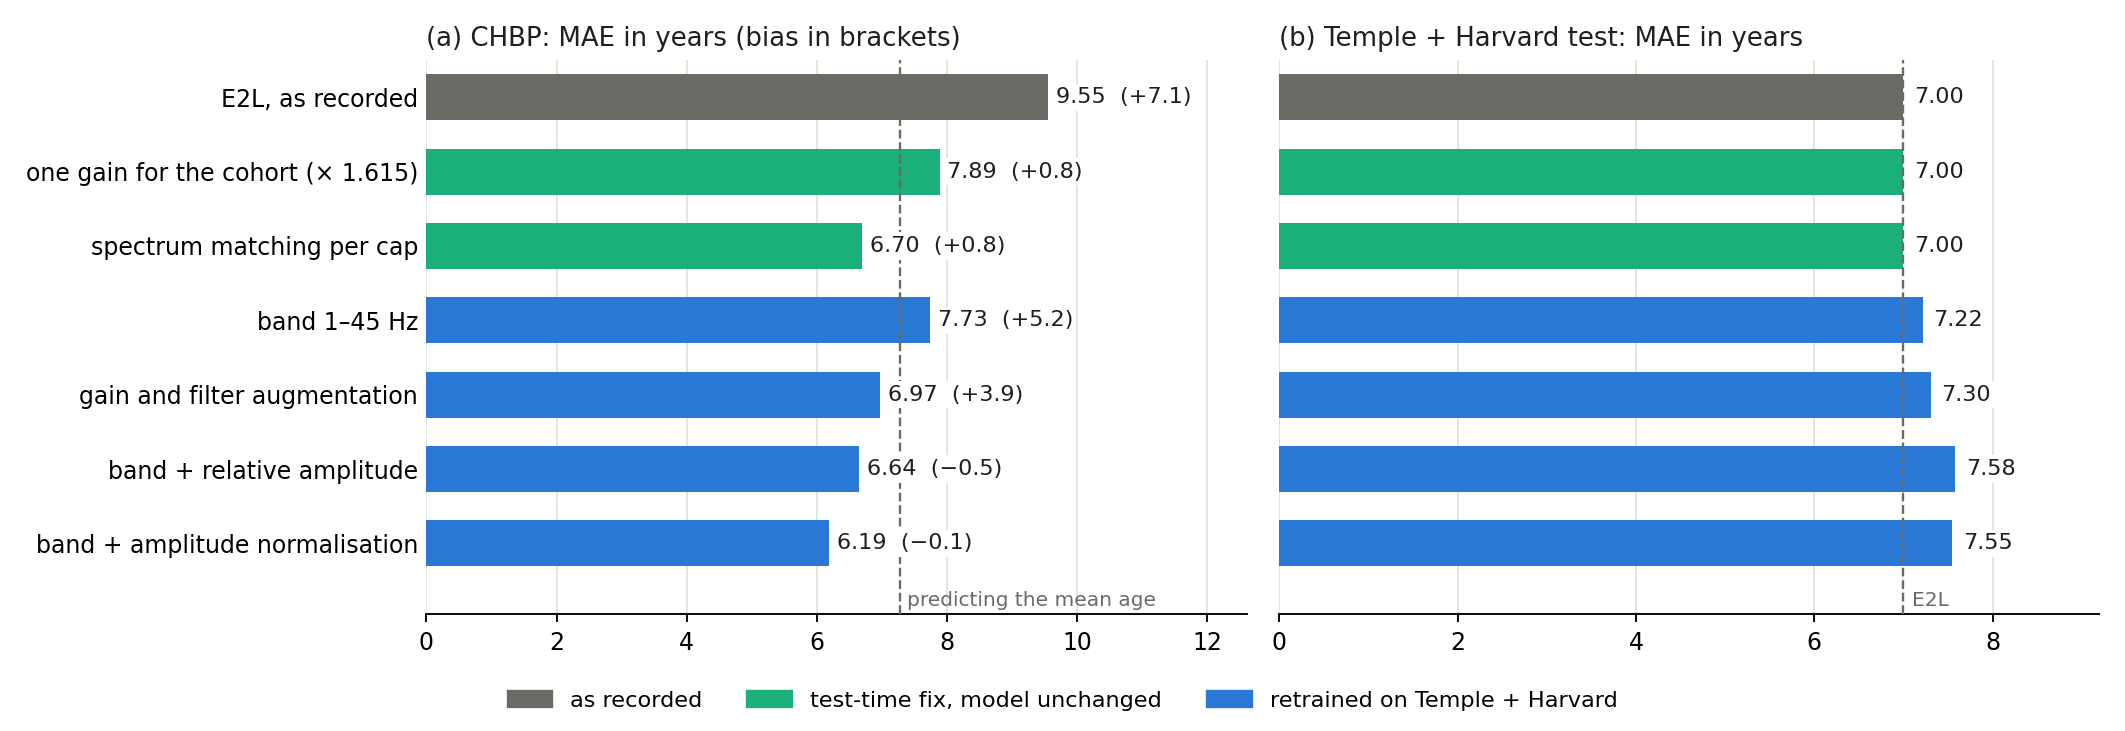
\includegraphics[width=\textwidth,height=0.62\textheight,keepaspectratio]{fig_chbp_fixes.png}
\caption{Corrections for CHBP: (a) MAE on CHBP with the bias in brackets, (b) MAE on the Temple + Harvard test split. Dashed: predicting CHBP's mean age in (a), E2L in (b).}
\end{figure}


What Table 27 and Figure 22 show:

\begin{itemize}
\item \textbf{The band limit restores the ranking, the amplitude sets the bias.} Band-limited training alone raises the correlation with age on CHBP from 0.44 to 0.55 but keeps an offset of +5 years; only a model that does not see the absolute amplitude removes the offset.
\item \textbf{The device-robust model is the best single correction.} It scores CHBP as recorded at 6.19 years (5.90 over every window, $R^2 = 0.33$), level with the best published result of a model trained on CHBP: 6.19 $\pm$ 1.10 against 6.48 $\pm$ 0.60 over the same ten folds~\citep{engemann2022benchmark}. The 120-channel cap gains most (13.10 $\rightarrow$ 6.67). The same model is unaffected by the transform of Eq. (24) (7.69 $\rightarrow$ 7.33 years).
\item \textbf{Augmentation teaches tolerance, not invariance.} The augmented model has the best ranking on CHBP (r 0.60) and stays closest to E2L in-domain among the amplitude-robust models (7.30), but it keeps a bias of +3.9 years: CHBP's gain of 0.6 sits at the edge of the range seen in training. Its training curves look like E2L's, with the gap between validation and clean training error growing to 2.6 years (E2L 2.85) and validation flat from epoch 11, so it overfits mildly and more epochs would not help; a wider gain range is the change to try.
\item \textbf{Robustness has a price.} Every variant that hides the absolute amplitude loses 1.6 to 2.1 years on young Harvard adults and about 0.9 years on LEMON: amplitude is a cue for young age. Giving it back as one number per recording does not recover the loss. No single retrained model matches E2L in-domain and corrects CHBP.
\item \textbf{Without retraining,} spectrum matching per cap takes E2L to 6.70 years, under the predict-the-mean level, at no in-domain cost; it needs a batch of unlabelled recordings of the new device.
\end{itemize}

The practical rule at present is two models and a label-free choice per cohort: E2L (or the ensembles of Section 4) for recordings inside the training range of amplitude and band, the device-robust model outside it. The attention ensembles were not retrained with these inputs; as recorded they reach 7.37 (P3) and 7.95 years (P4) on CHBP.

\subsection{Patients against controls inside a clinic cohort}

Three open clinic cohorts hold patients and healthy controls recorded in the same place: AHEPA~\citep{miltiadous2023ahepa} (36 Alzheimer's disease, 23 frontotemporal dementia, 29 controls; eyes closed, clinical Nihon Kohden system), Iowa~\citep{singh2023iowapd} (100 Parkinson's disease, 49 controls; eyes open, 2 to 6 minutes) and Tel Aviv~\citep{katzir2026telavivpd} (116 Parkinson's disease, 28 controls; eyes open, about 4 minutes). They fail as age benchmarks (Table 34): their controls, 61 to 71 years old on average, are predicted 7 to 11 years too young. Recordings of the training domain at the same ages are under-predicted by 1 to 6 years (the compression of Section 6.4), so 4 to 7 years remain unexplained; a gain or a band limit, the two causes found for CHBP, are not visible in their spectra (\texttt{docs/open\_cohorts\_onboarding.md} Section 6). Inside one cohort, patients and controls share the recording chain, the protocol and the recruitment, so a difference between them removes a shift common to both groups. We fit Eq. (22) with one linear age term in place of the age bands and heteroscedasticity-robust (HC3) standard errors, one recording per person (\texttt{scripts/clinical\_cohort\_gap.py}); the pooled Parkinson's estimate is the inverse-variance weighted mean of the two cohorts.

\begin{table}[t]
\centering
\small
\caption{Adjusted gap of each patient group against the controls of its own cohort: $\beta$ of Eq. (22) in years with a 95 \% interval, and p.}
\resizebox{\textwidth}{!}{%
\begin{tabular}{llllll}
\toprule
\textbf{cohort, group} & \textbf{patients / controls} & \textbf{E2L} & \textbf{device-robust E2L} & \textbf{P3 ensemble} & \textbf{P4 ensemble} \\
\midrule
AHEPA, Alzheimer's disease & 36 / 29 & +6.4 [1.1, 11.6], 0.02 & +7.5 [2.6, 12.3], 0.004 & +5.5 [$-$0.1, 11.1], 0.06 & +6.3 [1.0, 11.6], 0.02 \\
AHEPA, frontotemporal dementia & 23 / 29 & +5.3 [$-$0.8, 11.4], 0.09 & +5.0 [$-$0.5, 10.4], 0.08 & +4.3 [$-$2.0, 10.7], 0.19 & +4.8 [$-$1.2, 10.8], 0.13 \\
AHEPA, both & 59 / 29 & +5.7 [1.0, 10.3], 0.02 & +6.1 [1.9, 10.4], 0.006 & +4.7 [$-$0.2, 9.6], 0.06 & +5.4 [0.7, 10.0], 0.03 \\
Iowa, Parkinson's disease & 100 / 49 & +3.7 [0.0, 7.5], 0.05 & +1.8 [$-$1.1, 4.7], 0.24 & +3.2 [$-$0.6, 7.0], 0.10 & +3.0 [$-$0.4, 6.5], 0.09 \\
Tel Aviv, Parkinson's disease & 116 / 28 & +2.8 [$-$0.3, 5.9], 0.08 & +2.2 [$-$0.8, 5.2], 0.15 & +3.0 [$-$0.3, 6.3], 0.07 & +2.6 [$-$0.6, 5.8], 0.11 \\
Parkinson's disease, both cohorts pooled & 216 / 77 & +3.2 [0.8, 5.6] & +2.0 [$-$0.1, 4.1] & +3.1 [0.6, 5.6] & +2.8 [0.5, 5.2] \\
\bottomrule
\end{tabular}
}
\end{table}


What Table 28 shows:

\begin{itemize}
\item \textbf{Dementia patients look about 5 to 6 years older than the controls of the same clinic,} Alzheimer's disease 6.3 years with the P4 ensemble (p = 0.02); the direction and size are the same with all four models, and the interval is wide (1 to 12 years).
\item \textbf{Parkinson's disease: about 3 years, the same in two independent cohorts.} Neither cohort alone is significant; pooled, the interval excludes 0 for the raw-input models (+2.8 years [0.5, 5.2] for the P4 ensemble).
\item \textbf{The direction agrees with the hospital records of Table 15} (Harvard dementia +2.1 and movement disorders +1.8 years). The clinic estimates are larger, as expected for diagnosed, symptomatic patients (mean MMSE 18 and 22) against a diagnosis code anywhere in a hospital record.
\item \textbf{The gap does not track severity inside a group:} its partial correlation, given age, with MMSE, MoCA or UPDRS is between $-$0.14 and +0.13 (P4 ensemble; all p > 0.1).
\item \textbf{An abnormal EEG looks older in a third hospital too.} NMT~\citep{khan2022nmt}, routine clinical EEG released band-limited, is no age benchmark either (Table 34), but inside it the 145 adults with an abnormal report have a gap 3.1 years [1.8, 4.5] above that of the 1,217 with a normal report at the same age and sex (P4 ensemble; device-robust E2L +3.9 [2.3, 5.5]), against +1.8 to +2.6 in Temple and Harvard (Section 6.2).
\end{itemize}

Cautions. The groups are small, each estimate rests on one cohort's 28 to 49 controls, and the models are outside their reliable range on these cohorts: a contrast inside a cohort removes a shift common to both groups, not one that interacts with the disease. Medication is not controlled (the Parkinson's patients take levodopa). Nothing here is a diagnostic claim.

\subsection{The same people five years later, and the state of a session: Dortmund}

208 of the Dortmund participants were recorded again about 5 years later with the same setup, and every session holds four runs of the same person: eyes closed and eyes open, before and after a 2-hour block of cognitive tasks. With session predictions $\hat y_1, \hat y_2$ and ages $y_1, y_2$, the change of the prediction is $\Delta \hat y = \hat y_2 - \hat y_1$ against the elapsed time $\Delta y = y_2 - y_1$; for two run types of one session the paired difference of their predictions is defined the same way. The stability of the gap $g_j = \hat y_j - y_j$ is its Pearson correlation between the sessions and the intraclass correlation ICC(2,1) for absolute agreement.

\begin{table}[t]
\centering
\small
\caption{Paired differences of the predicted age in years, mean with a 95 \% bootstrap interval over people. Follow-up: 208 people, mean elapsed time 5.17 years; within a session: 815 sessions.}
\begin{tabular}{llll}
\toprule
\textbf{contrast} & \textbf{E2L} & \textbf{P3 ensemble} & \textbf{P4 ensemble} \\
\midrule
session 2 $-$ session 1 (5.17 years apart) & +4.34 [3.78, 4.87] & +4.42 [3.84, 4.97] & +4.32 [3.79, 4.85] \\
share of people predicted older at session 2 & 90 \% & 86 \% & 89 \% \\
after $-$ before the task block, eyes closed & +1.61 [1.31, 1.88] & +1.11 [0.75, 1.46] & +1.47 [1.14, 1.79] \\
after $-$ before the task block, eyes open & +2.20 [1.91, 2.48] & +1.72 [1.36, 2.05] & +1.72 [1.40, 2.01] \\
eyes open $-$ eyes closed, before the tasks & $-$0.15 [$-$0.53, 0.23] & $-$0.44 [$-$0.91, 0.03] & $-$0.12 [$-$0.54, 0.29] \\
eyes open $-$ eyes closed, after the tasks & +0.45 [0.13, 0.77] & +0.18 [$-$0.25, 0.57] & +0.14 [$-$0.23, 0.49] \\
\bottomrule
\end{tabular}
\end{table}


\begin{figure}[t]
\centering
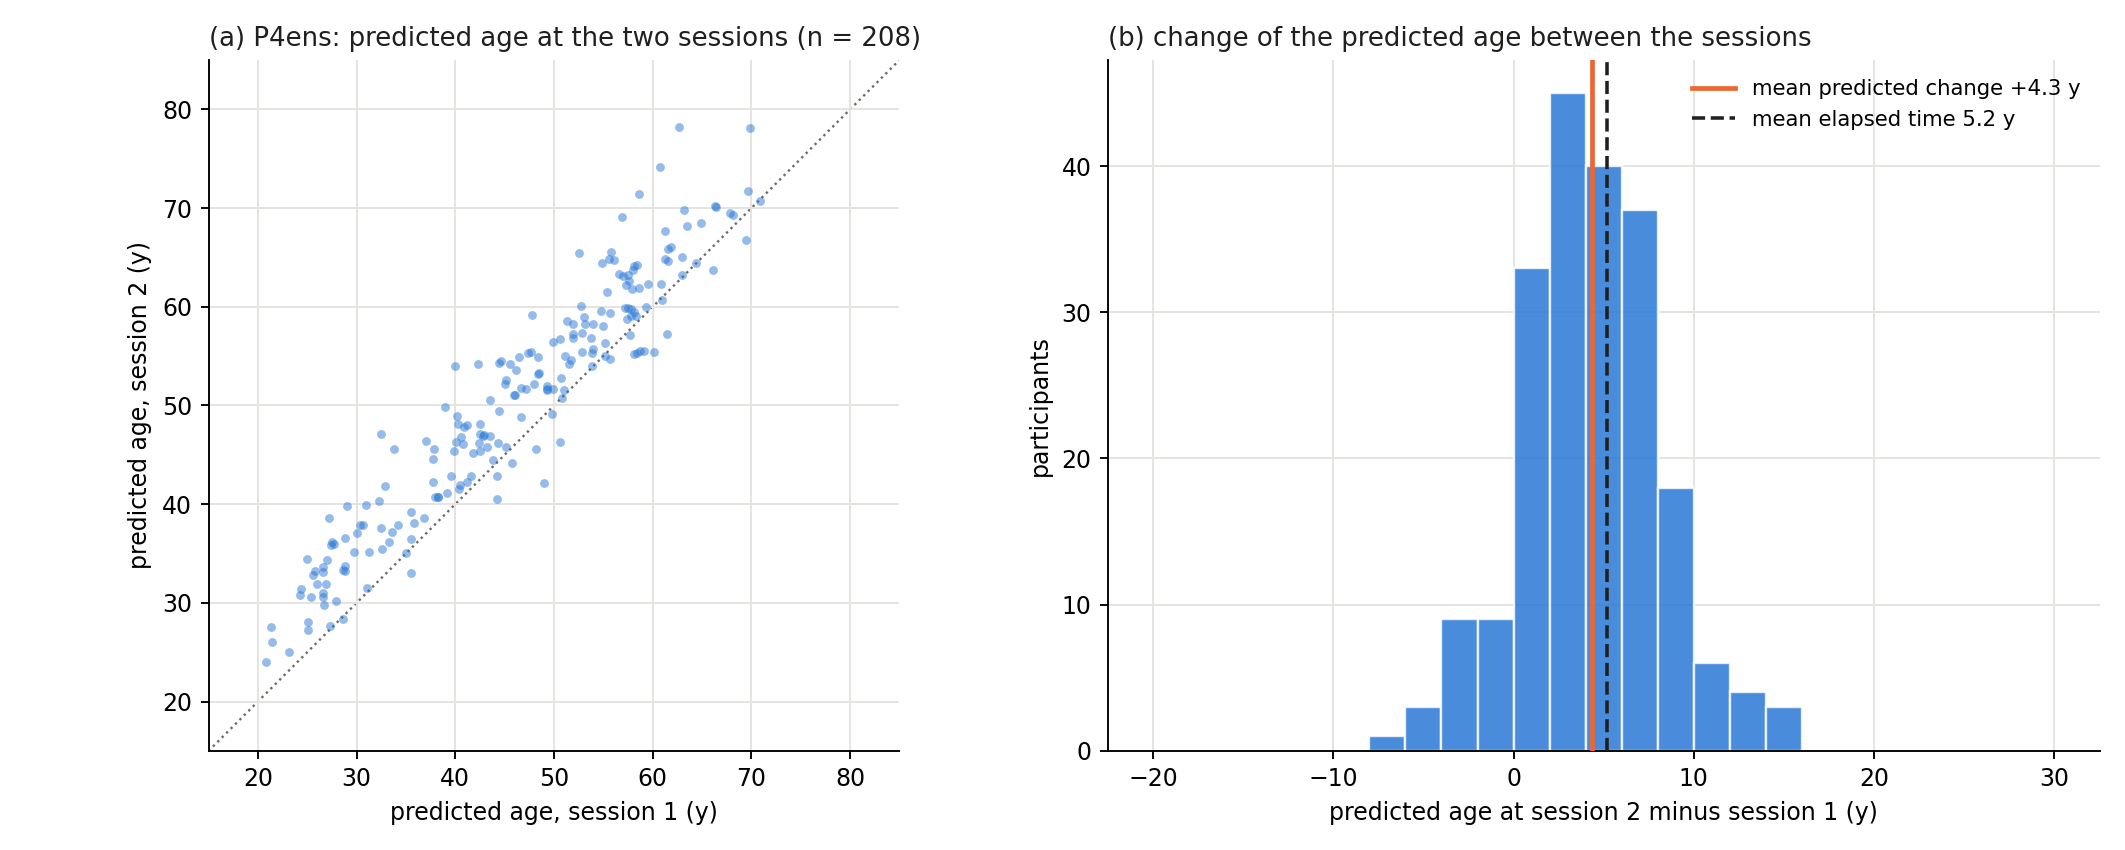
\includegraphics[width=\textwidth,height=0.62\textheight,keepaspectratio]{../figures/dortmund/dortmund_longitudinal.png}
\caption{Dortmund, P4 ensemble, 208 people with two sessions. (a) Predicted age at session 2 against session 1; dotted: identity. (b) Distribution of the change of the predicted age, with its mean (+4.3 years) and the mean elapsed time (5.2 years).}
\end{figure}


What Table 29 and Figure 23 show:

\begin{itemize}
\item \textbf{The models see people age.} The predicted age rises by 4.3 years over 5.2 years, and 89 \% of the participants are predicted older at the second session. The shortfall is the compression: the cross-sectional slope of the P4 prediction on age is 0.85 in Dortmund (Table 19), which predicts $0.85 \times 5.17 = 4.4$ years, so the change over time agrees with the cross-sectional relation.
\item \textbf{The gap is a property of the person.} Whoever looks older than their age at the first session still does 5 years later (P4 ensemble r = 0.77, ICC 0.77; E2L 0.79 and 0.78), almost as much as two parts of one visit 2 hours apart (r = 0.81). Gemein et al.~\citep{gemein2024revisited} found the same for repeated clinical recordings and read it as a trait.
\item \textbf{A single person's change is noisy.} The standard deviation of $\Delta \hat y$ is 3.9 years: the cohort ages visibly, but one person's 5-year change is within the noise of two 12-minute sessions.
\item \textbf{The state of the session moves the prediction.} After the 2-hour task block people look 1.5 to 1.7 years older with the P4 ensemble; with the amplitude-normalised model of Section 6.5 the shift is about half (0.8 to 1.2 years), so part of it goes with the larger post-task amplitude. Eyes open or closed does not shift the predicted age (within $\pm$0.5 years), although the two conditions differ strongly in alpha power, which supports pooling them as done for TDBRAIN.
\end{itemize}

The state shift is as large as many of the clinical effects of Tables 15 and 28, so a group comparison must fix the point of the session at which the EEG is recorded. Two cautions: the elapsed time is a difference of calendar years, known to $\pm$1 year per person, and a drift of the hardware over the 5 years would add to $\Delta \hat y$ and cannot be told apart from ageing here.

\section{Comparison with published work}

\begin{table}[t]
\centering
\small
\caption{Published EEG brain-age results on the test cohorts, and ours. "within" = trained and tested on the cohort with cross-validation; "zero-shot" = trained elsewhere and applied unchanged. MAE in years.}
\resizebox{\textwidth}{!}{%
\begin{tabular}{llllll}
\toprule
\textbf{cohort} & \textbf{study} & \textbf{method} & \textbf{protocol} & \textbf{MAE} & \textbf{$R^2$} \\
\midrule
TUAB & Gemein et al.~\citep{gemein2024revisited} & temporal convolutional network trained on normal recordings & within (train / eval) & 6.60 normal, 12.85 abnormal & not reported \\
TUAB & ours, P4 ensemble & Section 4 & in-domain, Temple test & 4.52 normal, 7.50 abnormal & 0.87, 0.67 \\
TDBRAIN & Khayretdinova et al.~\citep{khayretdinova2022tdbrain} & deep convolutional network on raw EEG & within, ages 5--88 & 5.96 & 0.81 \\
TDBRAIN & Hu et al.~\citep{hu2025neoba} & oscillatory features, sparse group lasso & protocol not stated for TDBRAIN, ages 5--89 & 4.95 & not reported \\
TDBRAIN & Bomatter et al.~\citep{bomatter2024biomarkers} & wavelet covariances, Riemannian / ridge models & within, ages 5--89 & not reported & about 0.8 \\
TDBRAIN & Hajhassani et al.~\citep{hajhassani2026artifact} & CNN-transformer with artifact removal, trained on Temple & zero-shot, healthy 20--90 & 8.36 & 0.59 \\
TDBRAIN & ours, P4 ensemble & Section 4 & zero-shot, adults 18--88 & 4.92 & 0.83 \\
LEMON & Engemann et al.~\citep{engemann2022benchmark} & Deep4Net (best of the benchmark) & within & 7.75 & 0.69 \\
LEMON & Mellot et al.~\citep{mellot2023harmonizing} & Riemannian model, without / with re-centring & trained on TUAB normals & not reported & 0.26 / 0.44 \\
LEMON & Hajhassani et al.~\citep{hajhassani2026artifact} & as above & zero-shot & 9.91 & 0.63 \\
LEMON & ours, P4 ensemble & Section 4 & zero-shot & 4.67 & 0.90 \\
Dortmund & Azami and Zandbagleh~\citep{azami2025dortmund} & spectral features & within, 10-fold CV, eyes open + closed; conference abstract & 2.24 & 0.91 \\
Dortmund & ours, P4 ensemble & Section 4 & zero-shot, sessions, 20--70 years & 4.53 & 0.85 \\
SRM & none found &  &  &  &  \\
SRM & ours, P3 ensemble & Section 4 & zero-shot & 4.75 & 0.79 \\
CHBP & Engemann et al.~\citep{engemann2022benchmark} & handcrafted features, random forest (best of the benchmark) & within & 6.48 & 0.18 \\
CHBP & ours, P3 ensemble / device-robust E2L & Section 4 / Section 6.5 & zero-shot & 7.37 / 5.90 & $-$0.14 / 0.33 \\
\bottomrule
\end{tabular}
}
\end{table}


How our approach differs from these studies:

\begin{itemize}
\item \textbf{Benchmark models}~\citep{engemann2022benchmark} and the TUAB network of Gemein et al.~\citep{gemein2024revisited} are trained within one cohort of a few hundred to a few thousand recordings, on cropped windows, with features or convolutional networks. We start from a self-supervised foundation encoder and train on about 100,000 hospital recordings, with a recording-level objective. Gemein et al. train on normal recordings only, which makes their abnormal error large by design; we train on all recordings and report both groups.
\item \textbf{TDBRAIN studies}~\citep{khayretdinova2022tdbrain,hu2025neoba,bomatter2024biomarkers} train on TDBRAIN itself and include children, whose ages widen the range and raise $R^2$. Our model never saw TDBRAIN and is scored on adults.
\item \textbf{Dortmund.} The one published result~\citep{azami2025dortmund} trains and tests inside the cohort; the abstract does not say whether a person's four runs stay in one fold, and with 3-minute runs of the same person in training and test folds a within-cohort MAE can be low for that reason alone. No zero-shot or cross-dataset age result on Dortmund or SRM was found.
\item \textbf{Cross-dataset studies.} Tveitstøl et al.~\citep{tveitstol2026robustness} train convolutional networks on four EEG datasets and test on a fifth, TDBRAIN and LEMON among them, and conclude that their models did not reach state-of-the-art performance across datasets. Hajhassani et al.~\citep{hajhassani2026artifact} train on Temple and test zero-shot with automated artifact removal; Mellot et al.~\citep{mellot2023harmonizing} need an unsupervised re-centring of the target cohort to transfer from TUAB to LEMON. Bikki and Zeng~\citep{bikki2026crossdataset} report an $R^2$ of 0.83 for a compact network applied zero-shot to TDBRAIN; only their abstract was available to us. We apply no alignment and no artifact removal to the target cohort.
\item \textbf{Confidence.} None of these studies reports a per-recording confidence or selective prediction.
\item \textbf{Psychiatric brain-age gap.} Structural MRI finds a small gap in major depression, +1.08 years (Cohen's d = 0.14) in the ENIGMA consortium~\citep{han2021enigma}. Our EEG result in TDBRAIN, no gap and a detectable difference of about 1.7 years, is compatible with an effect of that size.
\end{itemize}

Three cautions for these comparisons. The published studies use other subsets, age ranges and releases of the cohorts (for TDBRAIN the 2022 release, ours is release 3.1). LEMON's public ages are 5-year bins, which adds about 1.25 years to our MAE there. The term zero-shot is justified for the external cohorts: none of them is among the 16 pre-training sources of the LaBraM encoder, and our fine-tuning used Temple and Harvard only (Section 10.4).

\section{Limitations}

\begin{itemize}
\item \textbf{Old age and children.} Predictions are compressed toward the mean: for adults over 65 in TDBRAIN the P4 ensemble under-predicts by 5.4 years. Children are outside the training range and are over-predicted by 10 years or more (measured on a developmental cohort that is not part of this report).
\item \textbf{Recording chain.} CHBP shows that a narrower acquisition band and a lower amplitude are enough to bring the models to the predict-the-mean level. The robust variant fixes it at an in-domain cost; no single model does both. On a second shifted cohort, NMT, released band-limited to about 1--35 Hz, the raw-input models collapse (MAE 14.7 years or more) and the robust variant keeps part of the ranking (10.6 years, r 0.61), so the fix does not extend to bands narrower than its own 1--45 Hz input.
\item \textbf{Elderly controls of the clinic cohorts.} The healthy controls of AHEPA, Iowa and Tel Aviv are predicted 7 to 11 years too young, 4 to 7 years more than recordings of the training domain at the same ages, and the cause has not been found (population and state, eyes-open protocol and device are all possible). Healthy elderly volunteers of Dortmund do not show it.
\item \textbf{State of the recording.} In Dortmund the same person looks 1.5 to 1.7 years older after a 2-hour task block (Section 6.7). Recordings made at different points of a session, or after different activities, are not comparable at the level of the clinical effects. Whether CHBP's low amplitude comes from the amplifier gain, the electrodes or the export cannot be settled from the released data.
\item \textbf{Selection on test data.} The three rejection scores were chosen after comparing nine on the test cohorts, and the early ablations of Table 12 were selected on the TUAB test set. The rejection threshold of the main tables is the cohort's own score quantile, so it needs a batch of unlabelled recordings; thresholds fixed on validation (Section 10.4) keep 78 to 91 \% of a cohort at a similar error, but the total score has no validation counterpart, and no score flags a shifted cohort as a whole.
\item \textbf{Cross-validation groups.} The folds group Harvard recordings by the site-specific subject identifier; 326 patients seen at two sites (0.6 \% of the Harvard training and validation patients) fall into two folds (Section 3.3). The test split is grouped by patient and is not affected.
\item \textbf{Single runs.} E2L and each fold model are one seed. Differences between recipes below about 0.2 years (P3 against P4 in-domain) are within the fold-to-fold spread.
\item \textbf{Labels.} "Normal" and "abnormal" are EEG report verdicts, available for half of the Harvard recordings; TDBRAIN has indications but no EEG reports and no medication record. Harvard diagnoses are ICD-10 codes of the whole patient record and overlap (2.9 groups per diagnosed recording), so the rows of Table 15 are not independent effects, and they come from single fold models, not the ensemble.
\item \textbf{Data governance.} Harvard and TDBRAIN are under data use agreements without redistribution. Only aggregates are reported.
\end{itemize}

\section{Planned work}

\begin{itemize}
\item Fix the protocol before a paper: the validation-fixed thresholds of Section 10.4 as the rejection rule, the first 5 minutes of every recording as the evaluation window, a fixed point of the session (resting EEG before any task block), and three seeds for the final recipe.
\item A cohort-level shift detector: Section 10.4 shows that the per-recording confidence keeps 80 \% of CHBP; a label-free comparison of a new cohort's amplitude and spectrum with the training range (Section 6.5) has to decide between the standard and the device-robust model.
\item Group the cross-validation folds by the cross-site patient identifier (Section 3.3) and retrain the ensembles.
\item Reduce the old-age compression in training (age-balanced sampling or loss) instead of after the fact.
\item One model for both recording chains: the band limit and a wider gain augmentation (beyond the 0.55 to 1.8 range of Eq. (28)) in the phased ensemble training, checked on CHBP and NMT.
\item A dedicated abnormal / pathology head trained with the age head, to separate "older-looking" from "abnormal"; Table 15 says that the abnormal EEG, not the diagnosis, carries the gap.
\item Robust pooling of the window predictions (median or trimming by the deviation of Eq. (21)), since attention adds nothing on TDBRAIN, Dortmund, SRM and CHBP.
\item Find the cause of the offset of the elderly clinic controls (Section 6.6), with forward tests on training recordings made eyes-open-only and short, and the clinics' raw exports.
\item Add the TDBRAIN replication subjects and a paediatric cohort, to extend the test to the blinded diagnoses and to children.
\item Study the brain-age gap against clinical covariates in Harvard (diagnosis codes, medication), with the bias corrections of Section 4.6, and the Dortmund gap against the study's cognitive and lifestyle measures~\citep{gajewski2022dortmund}, using its stability over 5 years.
\end{itemize}

\section{Technical details and full tables}

This section gives the details behind three parts of the report: the two age-bias corrections that use the true age (Section 10.1), every test dataset that was scored, with the ones that were rejected and why (Section 10.2), and the full performance table of each test cohort (Section 10.3).

\subsection{Linear and quadratic gap correction (uses the true age)}

\textbf{What is corrected.} The brain-age gap of recording $r$ is $\delta_r = \hat y_r - y_r$. A regression model shrinks its predictions toward the mean age of its training data, so on healthy people the prediction follows the age with a slope $a < 1$ and the gap falls with age:

\begin{equation}
\hat y = a\,y + b + \varepsilon \quad \Rightarrow \quad \delta = (a - 1)\,y + b + \varepsilon, \qquad y^{*} = \frac{b}{1 - a} \tag{29}
\end{equation}

Below the age $y^{*}$ the model over-predicts on average, above it the model under-predicts. Two groups of different ages therefore have different mean gaps even when their brains do not differ, and a raw gap cannot be compared between them.

\textbf{Fit.} The trend is estimated once per model by ordinary least squares on a reference set $V$: the adult validation recordings of the training cohort with a normal EEG report (\texttt{labram/eval/age\_analysis.py::fit\_bias\_correction}). For E2L these are its validation predictions; for an ensemble, the predictions of the fold models on their own validation folds, pooled (four of the five fold models for P3, three for P4). No recording of a scored cohort enters the fit, and the same coefficients are applied to every cohort and subset.

\begin{equation}
(a,\,b) = \arg\min \sum_{v \in V} \big( \hat y_v - a\,y_v - b \big)^2, \qquad (c_0,\,c_1,\,c_2) = \arg\min \sum_{v \in V} \big( \delta_v - c_0 - c_1 y_v - c_2 y_v^2 \big)^2 \tag{30}
\end{equation}

\textbf{Correction.} The expected gap of a normal recording of the same age is subtracted from the gap. The linear form~\citep{beheshti2019bias,delange2020commentary} and the quadratic form of Gemein et al.~\citep{gemein2024revisited} are

\begin{equation}
\delta_r^{lin} = \delta_r - \big( (a - 1)\,y_r + b \big), \qquad \hat y_r^{lin} = y_r + \delta_r^{lin} \tag{31}
\end{equation}

\begin{equation}
\delta_r^{quad} = \delta_r - \big( c_0 + c_1 y_r + c_2 y_r^2 \big), \qquad \hat y_r^{quad} = y_r + \delta_r^{quad} \tag{32}
\end{equation}

These are Eq. (18) written for the gap. The corrected gap is a residual: how much older or younger the recording looks than a normal-report recording of the same age. Its mean over the reference set is 0 by construction.

\begin{table}[t]
\centering
\small
\caption{Fitted coefficients of Eq. (30) per model. $n$: reference recordings; $y^{*}$ of Eq. (29) in years.}
\resizebox{\textwidth}{!}{%
\begin{tabular}{llllllll}
\toprule
\textbf{model} & \textbf{n} & \textbf{a} & \textbf{b} & \textbf{$y^{*}$} & \textbf{$c_0$} & \textbf{$c_1$} & \textbf{$c_2$} \\
\midrule
E2L & 2,881 & 0.746 & 11.90 & 46.8 & 7.64 & $-$0.054 & $-$0.00204 \\
P3 ensemble & 20,030 & 0.813 & 8.86 & 47.3 & 2.02 & 0.135 & $-$0.00327 \\
P4 ensemble & 15,157 & 0.793 & 9.89 & 47.7 & 2.75 & 0.129 & $-$0.00339 \\
\bottomrule
\end{tabular}
}
\end{table}


\begin{table}[t]
\centering
\small
\caption{Expected gap of a normal-report recording at four ages, in years, from the coefficients of Table 31: the amount that Eqs. (31) and (32) subtract.}
\resizebox{\textwidth}{!}{%
\begin{tabular}{llllll}
\toprule
\textbf{model} & \textbf{form} & \textbf{age 20} & \textbf{age 40} & \textbf{age 60} & \textbf{age 80} \\
\midrule
E2L & linear & +6.8 & +1.7 & $-$3.4 & $-$8.5 \\
 & quadratic & +5.7 & +2.2 & $-$2.9 & $-$9.7 \\
P3 ensemble & linear & +5.1 & +1.4 & $-$2.4 & $-$6.1 \\
 & quadratic & +3.4 & +2.2 & $-$1.6 & $-$8.1 \\
P4 ensemble & linear & +5.7 & +1.6 & $-$2.5 & $-$6.7 \\
 & quadratic & +4.0 & +2.5 & $-$1.7 & $-$8.7 \\
\bottomrule
\end{tabular}
}
\end{table}


Table 32 shows the size of the effect: a normal 80-year-old is predicted 6 to 10 years too young and a normal 20-year-old 3 to 7 years too old, by a model whose overall bias is below 1 year. The quadratic term is negative for every model: the under-prediction grows faster in old age than a line allows, which is why the quadratic form leaves the smaller residual on the hospital cohorts.

\textbf{Why these two corrections need the true age, and what follows.} Eqs. (31) and (32) evaluate the trend at the true age $y_r$. Three consequences:

\begin{itemize}
\item They are not predictors. With the true age unknown they cannot be computed, so they cannot be used to estimate an age. Cole inversion and recalibration, Eq. (17), are the forms that need no age, and they cost accuracy (Table 19).
\item Their "MAE" is the mean absolute corrected gap, not an accuracy. It is lower than the raw MAE on most cohorts because the age trend has been removed with the help of the label, and it must not be compared with a published MAE.
\item The slope of the corrected prediction on age changes by a fixed amount. With $s$ the raw slope inside a cohort,
\end{itemize}

\begin{equation}
s^{lin} = s + (1 - a) \tag{33}
\end{equation}

so the correction gives slope 1 only where the cohort is compressed as much as the reference set ($s = a$). For the P4 ensemble $1 - a = 0.21$: Temple goes from 0.79 to 1.00, TDBRAIN from 0.89 to 1.09 (over-corrected) and CHBP from 0.53 to 0.74 (under-corrected), the values of Table 19.

\textbf{Use.} The corrected gap serves group comparisons. For two groups $A$ and $B$ of one cohort,

\begin{equation}
\Delta_{A-B} = \frac{1}{\lvert A \rvert} \sum_{r \in A} \delta_r^{corr} - \frac{1}{\lvert B \rvert} \sum_{r \in B} \delta_r^{corr} \tag{34}
\end{equation}

tested with Welch's t-test. Subtracting a fixed function of age from the gap is equivalent to using age as a covariate with coefficients fixed on the reference set, so it does not leak the group labels of the scored cohort.

\begin{table}[t]
\centering
\small
\caption{P4 ensemble, gap before and after the two corrections, by cohort and subset: mean gap in years / mean absolute gap in years / Pearson r of the gap with age (0 = no age trend left). Subsets: normal EEG report or healthy controls; abnormal report or patients.}
\resizebox{\textwidth}{!}{%
\begin{tabular}{llllll}
\toprule
\textbf{cohort} & \textbf{subset} & \textbf{n} & \textbf{raw} & \textbf{linear gap, Eq. (31)} & \textbf{quadratic gap, Eq. (32)} \\
\midrule
Temple & all & 272 & $-$0.4 / 5.87 / $-$0.48 & +0.3 / 5.34 / $-$0.00 & +0.2 / 5.15 / 0.05 \\
 & normal / healthy & 149 & $-$0.3 / 4.52 / $-$0.46 & $-$1.0 / 4.41 / 0.13 & $-$1.1 / 4.29 / 0.11 \\
 & abnormal / patients & 123 & $-$0.4 / 7.50 / $-$0.57 & +1.7 / 6.47 / $-$0.25 & +1.7 / 6.20 / $-$0.15 \\
Harvard & all & 7,338 & $-$0.1 / 5.94 / $-$0.43 & +1.2 / 5.66 / 0.09 & +1.4 / 5.57 / 0.14 \\
 & normal / healthy & 1,518 & +0.0 / 5.69 / $-$0.42 & +0.2 / 5.51 / 0.11 & +0.4 / 5.35 / 0.11 \\
 & abnormal / patients & 2,253 & $-$0.1 / 6.49 / $-$0.49 & +2.2 / 6.09 / $-$0.03 & +2.6 / 6.04 / 0.04 \\
 & no report & 3,567 & $-$0.2 / 5.70 / $-$0.42 & +0.9 / 5.45 / 0.13 & +1.1 / 5.36 / 0.18 \\
TDBRAIN & all & 1,113 & $-$0.8 / 4.92 / $-$0.28 & $-$1.3 / 5.24 / 0.23 & $-$1.5 / 5.14 / 0.18 \\
 & normal / healthy & 179 & $-$0.4 / 4.96 / $-$0.28 & $-$2.0 / 5.63 / 0.21 & $-$1.9 / 5.37 / 0.14 \\
 & abnormal / patients & 934 & $-$0.8 / 4.92 / $-$0.28 & $-$1.1 / 5.17 / 0.23 & $-$1.5 / 5.09 / 0.19 \\
LEMON & all & 214 & $-$0.8 / 4.67 / $-$0.55 & $-$2.5 / 4.87 / 0.14 & $-$2.0 / 4.58 / 0.07 \\
Dortmund & all (sessions) & 816 & $-$1.1 / 4.53 / $-$0.40 & $-$1.5 / 4.45 / 0.15 & $-$1.9 / 4.45 / 0.08 \\
SRM & all & 152 & $-$1.1 / 4.84 / $-$0.26 & $-$2.9 / 5.65 / 0.20 & $-$3.1 / 5.53 / 0.07 \\
CHBP & all & 250 & +3.8 / 7.95 / $-$0.44 & +0.4 / 7.13 / $-$0.26 & +0.6 / 7.26 / $-$0.35 \\
\bottomrule
\end{tabular}
}
\end{table}


Three things can be read from Table 33. First, the correction removes the trend where the models work: in the normal-report subsets of Temple and Harvard the correlation of the gap with age goes from $-$0.46 and $-$0.42 to +0.11 to +0.13. Second, it uncovers a group difference that the raw gap hides. Abnormal-report recordings are 10 to 13 years older than normal-report ones (58.0 against 44.6 years in Temple, 58.8 against 48.8 in Harvard), so their raw mean gaps are equal ($-$0.4 against $-$0.3, $-$0.1 against 0.0), while after the linear correction they look about 2.7 years older in Temple and 2.0 in Harvard (2.8 and 2.2 with the quadratic form). TDBRAIN patients and controls differ by 0.9 and 0.4 years, not significant. Third, the correction is one function of age and repairs nothing else: on TDBRAIN and SRM, which are less compressed than the reference set, it raises the mean absolute gap (TDBRAIN 4.92 to 5.24 years, SRM 4.84 to 5.65) and adds an offset of $-$1.3 and $-$2.9 years, and on CHBP the gap keeps a correlation of $-$0.26 with age.

\subsection{Test datasets: used and rejected}

Thirteen cohorts were converted with the training pipeline and scored. Cohorts were rejected as age benchmarks for three kinds of reason: (i) too few adult units for a stable estimate, (ii) a released signal whose band or scale differs from the training data in a way no model variant corrects, and (iii) healthy or normal-report subjects predicted with a cohort-wide offset of unknown cause. Table 34 lists every cohort with its status. Only adults are scored in every cohort: the training data has almost no patients under 18, and children are over-predicted by 10 years or more.

\begin{table}[t]
\centering
\small
\caption{Every scored cohort and its status. n: adult units (recordings, or sessions for TDBRAIN and Dortmund). MAE: P4 ensemble, years, all adults. The numbers of the rejected cohorts are given as the evidence for the rejection, not as results.}
\resizebox{\textwidth}{!}{%
\begin{tabular}{llllll}
\toprule
\textbf{cohort} & \textbf{n} & \textbf{age, mean} & \textbf{MAE} & \textbf{status} & \textbf{reason} \\
\midrule
Temple (TUH) & 272 & 50.7 & 5.87 & used (Table 38) & held-out patients of the training corpus \\
Harvard (HEEDB) & 7,338 & 54.1 & 5.94 & used (Table 39) & held-out patients of the training corpus \\
TDBRAIN & 1,113 & 45.2 & 4.92 & used (Table 35) & external, zero-shot \\
LEMON & 214 & 39.2 & 4.67 & used (Table 36) & external, zero-shot; ages public as 5-year bins \\
CHBP & 250 & 31.7 & 7.95 & used, as the recording-chain case (Table 37) & recorded 0.5--50 Hz at about 0.6 times the training amplitude; only the device-robust model works (5.90 years, Section 6.5) \\
Dortmund Vital Study & 816 & 46.1 & 4.53 & used (Table 40) & external, zero-shot; exact ages, 208 people with a 5-year follow-up (Section 6.7); kept test-only \\
SRM & 152 & 38.8 & 4.84 & used (Table 41) & external, zero-shot; the smallest cohort of the report \\
NMT & 1,362 & 38.0 & 14.70 & rejected as an age benchmark & released band-limited to about 1--35 Hz with an undocumented amplitude scale; bias +9.9 years, $R^2 = -0.11$; kept for the normal / abnormal contrast inside the cohort (Section 6.6) \\
AHEPA & 88 & 66.2 & 11.23 & rejected as an age benchmark & the 29 controls are predicted 9.6 years too young, cause unknown; fewer than 100 units; kept for the patient / control contrast (Table 28) \\
Iowa Parkinson's & 149 & 69.3 & 10.91 & rejected as an age benchmark & the 49 controls are predicted 10.9 years too young, cause unknown; kept for the patient / control contrast (Table 28) \\
Tel Aviv Parkinson's & 144 & 65.1 & 8.66 & rejected as an age benchmark & the 28 controls are predicted 7.0 years too young, cause unknown; kept for the patient / control contrast (Table 28) \\
MIPDB, adults & 31 & 27.5 & 7.36 & rejected & too few: the 95 \% interval of the MAE is more than 4 years wide \\
HBN, adults & — & — & — & rejected & a paediatric study whose adults span only 18--22 years; kept out of every report \\
\bottomrule
\end{tabular}
}
\end{table}


The three elderly disease cohorts share one failure: their healthy controls, 65 to 69 years old on average, are predicted 7 to 11 years too young, more than the age compression of Table 32 explains at that age (about $-$4 years). The cause has not been found, so the cohorts cannot measure accuracy; the difference between patients and controls of one cohort is not affected by a cohort-wide offset and remains usable (Section 6.6). NMT fails for a known reason, the band limit of the release: the same 1--35 Hz limit applied to Temple and Harvard recordings takes E2L from 5.3 to 12.6 years. The public datasets that were surveyed but not downloaded are listed in the project notes (\texttt{docs/tdbrain\_onboarding.md}, Section 23).

\subsection{Main performance tables per test cohort}

Tables 35 to 41 give, for each of the seven cohorts of this report, every model with and without rejection of the 20 \% least confident units (Section 4.5; the three scores are spread, total and learned). The 20 \% are set aside in the whole cohort and the kept units are then split by subset. MAE in years with a 95 \% interval over 2,000 bootstrap resamples of subjects; $R^2$ and r of Eq. (19); bias is the mean gap in years; subset cells are MAE with $R^2$ in brackets. E2L is a single model and has only the spread score. The MAE of predicting the cohort's mean age is given in each caption as the reference. Published results on the same cohorts are in Table 30.

\begin{table}[t]
\centering
\small
\caption{TDBRAIN, adults, zero-shot: 1,113 sessions of 1,062 subjects, mean age 45.2 years; healthy controls 179 sessions (40.3 years), patients 934 (46.2 years). Predicting the mean age: 13.35 years.}
\resizebox{\textwidth}{!}{%
\begin{tabular}{lllllll}
\toprule
\textbf{model} & \textbf{rejected} & \textbf{MAE, all [95 \%]} & \textbf{$R^2$ / r} & \textbf{bias} & \textbf{healthy, MAE ($R^2$)} & \textbf{pathological, MAE ($R^2$)} \\
\midrule
E2L & none & 5.32 [5.04, 5.60] & 0.80 / 0.90 & $-$1.5 & 5.28 (0.81) & 5.33 (0.80) \\
 & 20 \%, spread & 5.02 [4.72, 5.31] & 0.83 / 0.92 & $-$1.5 & 4.49 (0.85) & 5.12 (0.82) \\
P3 ensemble & none & 5.14 [4.89, 5.41] & 0.82 / 0.91 & $-$1.0 & 5.15 (0.81) & 5.14 (0.81) \\
 & 20 \%, spread & 4.83 [4.56, 5.12] & 0.85 / 0.93 & $-$1.0 & 4.65 (0.85) & 4.87 (0.84) \\
 & 20 \%, total & 4.69 [4.43, 4.97] & 0.85 / 0.93 & $-$1.1 & 4.50 (0.84) & 4.72 (0.85) \\
 & 20 \%, learned & 4.74 [4.46, 5.04] & 0.84 / 0.92 & $-$1.1 & 4.63 (0.82) & 4.76 (0.84) \\
P4 ensemble & none & 4.92 [4.68, 5.19] & 0.83 / 0.91 & $-$0.8 & 4.96 (0.82) & 4.92 (0.83) \\
 & 20 \%, spread & 4.54 [4.27, 4.81] & 0.86 / 0.93 & $-$0.7 & 4.32 (0.87) & 4.58 (0.86) \\
 & 20 \%, total & 4.53 [4.26, 4.81] & 0.86 / 0.93 & $-$0.8 & 4.24 (0.86) & 4.58 (0.86) \\
 & 20 \%, learned & 4.57 [4.30, 4.85] & 0.86 / 0.93 & $-$0.8 & 4.43 (0.84) & 4.60 (0.86) \\
\bottomrule
\end{tabular}
}
\end{table}


\begin{table}[t]
\centering
\small
\caption{LEMON, adults, zero-shot: 214 subjects, mean age 39.2 years, all healthy volunteers. Predicting the mean age: 18.60 years.}
\resizebox{\textwidth}{!}{%
\begin{tabular}{lllll}
\toprule
\textbf{model} & \textbf{rejected} & \textbf{MAE, all [95 \%]} & \textbf{$R^2$ / r} & \textbf{bias} \\
\midrule
E2L & none & 5.20 [4.60, 5.84] & 0.88 / 0.95 & $-$0.8 \\
 & 20 \%, spread & 4.37 [3.81, 4.93] & 0.90 / 0.96 & $-$0.5 \\
P3 ensemble & none & 4.70 [4.17, 5.29] & 0.90 / 0.95 & $-$1.0 \\
 & 20 \%, spread & 3.86 [3.34, 4.38] & 0.92 / 0.96 & $-$1.0 \\
 & 20 \%, total & 4.02 [3.50, 4.57] & 0.92 / 0.96 & $-$0.7 \\
 & 20 \%, learned & 3.80 [3.31, 4.32] & 0.92 / 0.96 & $-$0.6 \\
P4 ensemble & none & 4.67 [4.11, 5.24] & 0.90 / 0.95 & $-$0.8 \\
 & 20 \%, spread & 3.79 [3.28, 4.30] & 0.93 / 0.97 & $-$0.7 \\
 & 20 \%, total & 3.80 [3.32, 4.30] & 0.93 / 0.96 & $-$0.4 \\
 & 20 \%, learned & 3.81 [3.32, 4.34] & 0.92 / 0.96 & $-$0.4 \\
\bottomrule
\end{tabular}
}
\end{table}


\begin{table}[t]
\centering
\small
\caption{CHBP, adults, zero-shot: 250 subjects, mean age 31.7 years, all healthy volunteers. Predicting the mean age: 7.27 years.}
\resizebox{\textwidth}{!}{%
\begin{tabular}{lllll}
\toprule
\textbf{model} & \textbf{rejected} & \textbf{MAE, all [95 \%]} & \textbf{$R^2$ / r} & \textbf{bias} \\
\midrule
E2L & none & 9.35 [8.45, 10.27] & $-$0.64 / 0.45 & +7.0 \\
 & 20 \%, spread & 9.23 [8.20, 10.30] & $-$0.87 / 0.42 & +6.8 \\
P3 ensemble & none & 7.37 [6.60, 8.28] & $-$0.14 / 0.48 & +2.7 \\
 & 20 \%, spread & 7.02 [6.13, 7.94] & $-$0.17 / 0.47 & +2.0 \\
 & 20 \%, total & 6.18 [5.43, 7.03] & 0.00 / 0.49 & +1.2 \\
 & 20 \%, learned & 6.49 [5.67, 7.30] & $-$0.01 / 0.51 & +1.5 \\
P4 ensemble & none & 7.95 [7.11, 8.87] & $-$0.28 / 0.49 & +3.8 \\
 & 20 \%, spread & 7.84 [6.91, 8.83] & $-$0.42 / 0.48 & +3.3 \\
 & 20 \%, total & 7.03 [6.17, 7.89] & $-$0.11 / 0.52 & +2.4 \\
 & 20 \%, learned & 7.43 [6.53, 8.37] & $-$0.29 / 0.47 & +2.8 \\
\bottomrule
\end{tabular}
}
\end{table}


\begin{table}[t]
\centering
\small
\caption{Temple (TUH), adults, in-domain test: 272 recordings of 249 patients, mean age 50.7 years; normal EEG report 149 recordings (44.6 years), abnormal report 123 (58.0 years). Predicting the mean age: 14.83 years.}
\resizebox{\textwidth}{!}{%
\begin{tabular}{lllllll}
\toprule
\textbf{model} & \textbf{rejected} & \textbf{MAE, all [95 \%]} & \textbf{$R^2$ / r} & \textbf{bias} & \textbf{normal report, MAE ($R^2$)} & \textbf{abnormal report, MAE ($R^2$)} \\
\midrule
E2L & none & 6.40 [5.75, 7.09] & 0.78 / 0.89 & $-$0.8 & 4.91 (0.85) & 8.21 (0.62) \\
 & 20 \%, spread & 5.87 [5.23, 6.54] & 0.83 / 0.92 & $-$1.1 & 4.88 (0.85) & 7.25 (0.70) \\
P3 ensemble & none & 5.87 [5.24, 6.52] & 0.81 / 0.90 & $-$0.5 & 4.61 (0.87) & 7.39 (0.67) \\
 & 20 \%, spread & 5.44 [4.84, 6.09] & 0.85 / 0.92 & $-$0.7 & 4.64 (0.86) & 6.59 (0.76) \\
 & 20 \%, total & 5.07 [4.47, 5.69] & 0.86 / 0.93 & $-$0.8 & 4.44 (0.88) & 6.20 (0.75) \\
 & 20 \%, learned & 4.97 [4.38, 5.60] & 0.87 / 0.93 & $-$0.8 & 4.29 (0.88) & 6.15 (0.78) \\
P4 ensemble & none & 5.87 [5.25, 6.54] & 0.81 / 0.90 & $-$0.4 & 4.52 (0.87) & 7.50 (0.67) \\
 & 20 \%, spread & 5.69 [5.02, 6.42] & 0.84 / 0.92 & $-$0.6 & 4.62 (0.87) & 7.26 (0.72) \\
 & 20 \%, total & 5.07 [4.44, 5.69] & 0.87 / 0.93 & $-$0.8 & 4.40 (0.87) & 6.32 (0.78) \\
 & 20 \%, learned & 5.11 [4.52, 5.68] & 0.86 / 0.93 & $-$0.7 & 4.46 (0.87) & 6.22 (0.78) \\
\bottomrule
\end{tabular}
}
\end{table}


\begin{table}[t]
\centering
\small
\caption{Harvard (HEEDB), adults, in-domain test: 7,338 recordings of 5,884 patients, mean age 54.1 years; normal EEG report 1,518 recordings (48.8 years), abnormal 2,253 (58.8 years), no report 3,567 (53.3 years). Predicting the mean age: 16.94 years.}
\resizebox{\textwidth}{!}{%
\begin{tabular}{llllllll}
\toprule
\textbf{model} & \textbf{rejected} & \textbf{MAE, all [95 \%]} & \textbf{$R^2$ / r} & \textbf{bias} & \textbf{normal, MAE ($R^2$)} & \textbf{abnormal, MAE ($R^2$)} & \textbf{no report, MAE ($R^2$)} \\
\midrule
E2L & none & 7.02 [6.88, 7.16] & 0.79 / 0.90 & $-$0.6 & 7.12 (0.78) & 7.56 (0.75) & 6.64 (0.81) \\
 & 20 \%, spread & 6.76 [6.60, 6.93] & 0.77 / 0.88 & $-$1.2 & 6.71 (0.75) & 7.33 (0.69) & 6.45 (0.81) \\
P3 ensemble & none & 5.98 [5.86, 6.12] & 0.84 / 0.91 & $-$0.1 & 5.73 (0.84) & 6.52 (0.80) & 5.74 (0.85) \\
 & 20 \%, spread & 5.61 [5.46, 5.75] & 0.86 / 0.93 & $-$0.1 & 5.27 (0.87) & 6.13 (0.83) & 5.42 (0.87) \\
 & 20 \%, total & 5.39 [5.25, 5.53] & 0.88 / 0.94 & $-$0.1 & 5.27 (0.87) & 5.84 (0.85) & 5.19 (0.89) \\
 & 20 \%, learned & 5.33 [5.20, 5.46] & 0.88 / 0.94 & $-$0.2 & 5.13 (0.88) & 5.82 (0.86) & 5.12 (0.89) \\
P4 ensemble & none & 5.94 [5.82, 6.07] & 0.84 / 0.92 & $-$0.1 & 5.69 (0.84) & 6.49 (0.80) & 5.70 (0.85) \\
 & 20 \%, spread & 5.56 [5.42, 5.71] & 0.87 / 0.93 & $-$0.2 & 5.27 (0.87) & 6.09 (0.83) & 5.36 (0.88) \\
 & 20 \%, total & 5.32 [5.19, 5.45] & 0.88 / 0.94 & $-$0.2 & 5.23 (0.87) & 5.75 (0.85) & 5.11 (0.89) \\
 & 20 \%, learned & 5.34 [5.20, 5.47] & 0.88 / 0.94 & $-$0.3 & 5.18 (0.88) & 5.77 (0.86) & 5.15 (0.89) \\
\bottomrule
\end{tabular}
}
\end{table}


\begin{table}[t]
\centering
\small
\caption{Dortmund Vital Study, adults, zero-shot: 816 sessions of 608 people (four 3-minute runs each), mean age 46.1 years, all healthy volunteers. Predicting the mean age: 12.74 years.}
\resizebox{\textwidth}{!}{%
\begin{tabular}{lllll}
\toprule
\textbf{model} & \textbf{rejected} & \textbf{MAE, all [95 \%]} & \textbf{$R^2$ / r} & \textbf{bias} \\
\midrule
E2L & none & 5.01 [4.70, 5.36] & 0.81 / 0.91 & $-$2.1 \\
 & 20 \%, spread & 4.71 [4.40, 5.02] & 0.84 / 0.93 & $-$1.8 \\
P3 ensemble & none & 4.72 [4.45, 5.01] & 0.83 / 0.92 & $-$1.6 \\
 & 20 \%, spread & 4.52 [4.23, 4.84] & 0.85 / 0.93 & $-$1.5 \\
 & 20 \%, total & 4.45 [4.16, 4.75] & 0.86 / 0.93 & $-$1.5 \\
 & 20 \%, learned & 4.50 [4.20, 4.81] & 0.85 / 0.93 & $-$1.4 \\
P4 ensemble & none & 4.53 [4.25, 4.82] & 0.85 / 0.92 & $-$1.1 \\
 & 20 \%, spread & 4.24 [3.97, 4.54] & 0.87 / 0.94 & $-$0.9 \\
 & 20 \%, total & 4.32 [4.03, 4.63] & 0.87 / 0.93 & $-$1.0 \\
 & 20 \%, learned & 4.32 [4.03, 4.62] & 0.86 / 0.93 & $-$0.9 \\
\bottomrule
\end{tabular}
}
\end{table}


\begin{table}[t]
\centering
\small
\caption{SRM, adults, zero-shot: 152 recordings of 110 people, mean age 38.8 years, all healthy volunteers. Predicting the mean age: 11.27 years.}
\resizebox{\textwidth}{!}{%
\begin{tabular}{lllll}
\toprule
\textbf{model} & \textbf{rejected} & \textbf{MAE, all [95 \%]} & \textbf{$R^2$ / r} & \textbf{bias} \\
\midrule
E2L & none & 5.01 [4.37, 5.70] & 0.77 / 0.88 & $-$0.1 \\
 & 20 \%, spread & 4.66 [3.99, 5.38] & 0.82 / 0.91 & $-$0.2 \\
P3 ensemble & none & 4.75 [4.13, 5.42] & 0.79 / 0.90 & $-$1.3 \\
 & 20 \%, spread & 4.57 [3.91, 5.29] & 0.81 / 0.91 & $-$1.8 \\
 & 20 \%, total & 4.42 [3.74, 5.20] & 0.81 / 0.91 & $-$1.7 \\
 & 20 \%, learned & 4.43 [3.74, 5.14] & 0.80 / 0.91 & $-$1.7 \\
P4 ensemble & none & 4.84 [4.23, 5.50] & 0.79 / 0.89 & $-$1.1 \\
 & 20 \%, spread & 4.60 [3.89, 5.35] & 0.82 / 0.91 & $-$1.3 \\
 & 20 \%, total & 4.60 [3.95, 5.30] & 0.81 / 0.91 & $-$1.1 \\
 & 20 \%, learned & 4.39 [3.70, 5.07] & 0.81 / 0.91 & $-$1.0 \\
\bottomrule
\end{tabular}
}
\end{table}


What the seven tables show together:

\begin{itemize}
\item \textbf{Accuracy without rejection.} The P4 ensemble reaches 4.53 to 4.92 years zero-shot on LEMON, TDBRAIN, Dortmund and SRM and 5.87 to 5.94 years on the held-out hospital recordings; in every cohort but CHBP this is 25 to 43 \% of the error of predicting the mean age.
\item \textbf{Healthy against pathological.} In Temple an abnormal report raises the MAE from 4.52 to 7.50 years, in Harvard from 5.69 to 6.49; Harvard recordings without a report behave like the normal ones (5.70). In TDBRAIN patients and controls are predicted equally well (4.92 against 4.96).
\item \textbf{Rejection.} Setting aside 20 \% lowers the MAE of the P4 ensemble by 0.4 years on TDBRAIN, 0.9 on LEMON, 0.2 on Dortmund and SRM, 0.8 on Temple and 0.6 on Harvard with the total score; no score is best on every cohort.
\item \textbf{CHBP.} Every model has $R^2 \le 0$ and a bias of +2.7 to +7.0 years; rejection lowers the MAE, but the best case (P3 ensemble, total score) only reaches $R^2 = 0.00$.
\end{itemize}

\subsection{A fixed protocol: evaluation window, rejection thresholds and pre-training overlap}

The main tables use two protocol choices that a paper should fix: in-domain cohorts are scored on their first 5 minutes and external cohorts on every window, and the rejection threshold is the cohort's own 80 \% score quantile. This section scores every cohort under one window and with thresholds fixed on validation data, and checks the pre-training data of the encoder against every test cohort (\texttt{scripts/report\_protocol.py}, \texttt{docs/data/external\_eval/tech\_report/protocol\_*.csv}).

\textbf{Evaluation window.} The windows that start in the first $m$ minutes of a recording form the set $W_m$. Fold model $k$'s prediction from them is

\begin{equation}
\hat y_{r,k}^{(m)} = \frac{\sum_{i \in W_m} \alpha_i \, p_i}{\sum_{i \in W_m} \alpha_i} \tag{35}
\end{equation}

with $p_i$ and $\alpha_i$ the window predictions and attention weights saved when every window was scored. Eq. (35) is exact, not an approximation: the softmax of Eq. (10) renormalises over the kept windows, and the head is linear, so $g\big(\sum_i \alpha_i h_{r,i}\big) = \sum_i \alpha_i\, g(h_{r,i})$ when $\sum_i \alpha_i = 1$. It reproduces the stored predictions to within 0.01 years. For E2L the weights are uniform. The in-domain ensembles were saved for the first 5 minutes only; E2L was also scored on every window in-domain.

\begin{table}[t]
\centering
\small
\caption{MAE in years by evaluation window. In-domain: after the 60 s trims. "—": not saved. TDBRAIN, Dortmund and SRM runs are at most 5 minutes long, so their 5-minute window holds every window.}
\resizebox{\textwidth}{!}{%
\begin{tabular}{lllllll}
\toprule
\textbf{cohort} & \textbf{E2L, 2 min} & \textbf{E2L, 5 min} & \textbf{E2L, every window} & \textbf{P4, 2 min} & \textbf{P4, 5 min} & \textbf{P4, every window} \\
\midrule
Temple & 6.33 & 6.40 & 6.35 & 5.96 & 5.87 & — \\
Harvard & 8.32 & 7.02 & 6.12 & 6.61 & 5.94 & — \\
TDBRAIN & 5.32 & 5.32 & 5.32 & 4.92 & 4.92 & 4.92 \\
LEMON & 5.33 & 5.22 & 5.20 & 4.85 & 4.80 & 4.67 \\
Dortmund & 5.00 & 5.01 & 5.01 & 4.52 & 4.53 & 4.53 \\
SRM & 5.12 & 5.01 & 5.01 & 4.80 & 4.84 & 4.84 \\
CHBP & 9.58 & 9.55 & 9.35 & 8.54 & 8.38 & 7.95 \\
\bottomrule
\end{tabular}
}
\end{table}


What Table 42 shows:

\begin{itemize}
\item \textbf{The main tables slightly favour the two long external recordings.} Scored on the first 5 minutes, as in-domain, the P4 ensemble gives 4.80 instead of 4.67 years on LEMON and 8.38 instead of 7.95 on CHBP; the three short cohorts do not change.
\item \textbf{The in-domain numbers are conservative.} Every window of a Harvard recording (about 30 minutes) takes E2L from 7.02 to 6.12 years, more than the 0.1 to 0.4 years the long external recordings gain.
\item \textbf{Two minutes are too few in-domain:} 6.61 instead of 5.94 years on Harvard (P4).
\end{itemize}

A fixed protocol of the first 5 minutes changes no external MAE of Table 13 by more than 0.43 years and keeps the order of the models on every cohort; it is the rule we propose for a paper.

\textbf{Rejection thresholds fixed on validation.} For a score with a single-model form, the threshold is the 80 \% quantile over the validation recordings $V_k$ of each fold model $k$, on its own validation fold (adults, first 5 minutes; for the P4 ensemble 57,111 recordings of three fold models):

\begin{equation}
\tau = Q_{0.8}\big\{\, c_{v,k} : v \in V_k,\ k \,\big\}, \qquad \text{keep } r \Leftrightarrow \frac{1}{K}\sum_{k} c_{r,k} \le \tau \tag{36}
\end{equation}

$c$ is the spread of Eq. (13), or the learned score: the predicted absolute error of the gradient-boosted regressor of Section 4.5, without the rank average with $d_r$. On validation each fold model's recordings are predicted by a regressor fitted on the other fold models' validation folds, so the threshold is not set on fitted values. The combined score of Eq. (14) has no validation form, because on validation every recording is seen by one fold model only. The thresholds for the P4 ensemble are 7.23 years (spread) and 6.03 years (learned). On validation, keeping 80 \% lowers the MAE from 6.62 to 6.25 and 6.09 years.

\begin{table}[t]
\centering
\small
\caption{P4 ensemble, first 5 minutes: MAE in years of the kept units, with the share kept, under each rule of Eq. (36) and under the cohort's own 80 \% quantile of the same score.}
\resizebox{\textwidth}{!}{%
\begin{tabular}{llllllll}
\toprule
\textbf{rule} & \textbf{Temple} & \textbf{Harvard} & \textbf{TDBRAIN} & \textbf{LEMON} & \textbf{Dortmund} & \textbf{SRM} & \textbf{CHBP} \\
\midrule
no rejection & 5.87 & 5.94 & 4.92 & 4.80 & 4.53 & 4.84 & 8.38 \\
spread, cohort quantile & 5.69 (80 \%) & 5.56 (80 \%) & 4.54 (80 \%) & 3.96 (80 \%) & 4.24 (80 \%) & 4.60 (80 \%) & 8.17 (80 \%) \\
spread, validation threshold & 5.58 (88 \%) & 5.57 (80 \%) & 4.64 (89 \%) & 4.10 (89 \%) & 4.40 (90 \%) & 4.55 (82 \%) & 8.24 (78 \%) \\
learned, cohort quantile & 5.46 (80 \%) & 5.28 (80 \%) & 4.58 (80 \%) & 4.06 (80 \%) & 4.27 (80 \%) & 4.56 (80 \%) & 7.92 (80 \%) \\
learned, validation threshold & 5.53 (83 \%) & 5.29 (81 \%) & 4.71 (91 \%) & 4.10 (87 \%) & 4.42 (91 \%) & 4.66 (84 \%) & 7.90 (80 \%) \\
\bottomrule
\end{tabular}
}
\end{table}


What Table 43 shows:

\begin{itemize}
\item \textbf{The thresholds transfer within the domain.} Harvard, whose test patients are exchangeable with the validation patients, keeps 80 and 81 \%, as intended; Temple keeps 83 to 88 \%.
\item \textbf{The external cohorts of volunteers and outpatients keep more, 82 to 91 \%,} and the kept units are within $-$0.05 to +0.16 years of the cohort-quantile rule, which rejects more: cleaner recordings are less uncertain, and a fixed threshold says so.
\item \textbf{A shifted cohort is not recognised.} CHBP, with twice the error of the other cohorts, keeps 78 to 80 \%: the scores measure the disagreement of windows and of fold models, not the distance of a cohort from the training data. The choice between the standard and the device-robust model (Section 6.5) needs a cohort-level check of amplitude and spectrum, not the per-recording confidence.
\end{itemize}

\textbf{Pre-training data.} The LaBraM encoder was pre-trained on 2,534.78 hours from 16 sources, listed in Appendix D of its paper~\citep{jiang2024labram}: BCI Competition IV-1, Emobrain, Grasp and Lift, Inria BCI Challenge, EEG Motor Movement/Imagery, Raw EEG Data (Trujillo 2020), Resting State EEG Data (Trujillo et al. 2017, 22 subjects), the SEED series, the Siena Scalp EEG Database, the SPIS Resting State Dataset, Target versus Non-Target, the four Temple subsets TUAR, TUEP, TUSZ and TUSL, and the authors' own recordings. Table 44 checks each test cohort.

\begin{table}[t]
\centering
\small
\caption{Test cohorts in the pre-training data of the LaBraM encoder. Self-supervised: the encoder saw the signals without any age label.}
\begin{tabular}{lll}
\toprule
\textbf{cohort} & \textbf{in LaBraM's pre-training} & \textbf{consequence} \\
\midrule
Temple & partly: 127 of the 272 test recordings are in TUSZ, TUEP, TUAR or TUSL & no measurable advantage (below) \\
Harvard & no &  \\
TDBRAIN, LEMON, Dortmund, SRM, CHBP & no & zero-shot in the strict sense \\
AHEPA, Iowa, Tel Aviv, NMT & no &  \\
\bottomrule
\end{tabular}
\end{table}


The 127 Temple recordings seen in pre-training are not predicted better: MAE 6.03 against 5.73 years for the other 145 (P4 ensemble); they are older (52.2 against 49.3 years) and more often abnormal (58 against 34 \%). With age, age squared and the report as covariates, their extra absolute error is $-$0.34 years [$-$1.53, 0.90] (P4) and +0.15 [$-$1.08, 1.35] (E2L), intervals from 2,000 bootstrap resamples of patients. Other EEG foundation models were pre-trained on some of our external cohorts (REVE on NMT and SRM, LEAD on Dortmund and the Iowa set; \texttt{docs/tdbrain\_onboarding.md} Table 35.2), so the zero-shot status holds for the LaBraM checkpoint only and would have to be re-checked for other initial weights.

\bibliographystyle{unsrtnat}
\bibliography{refs}
\end{document}
